% !Mode:: "Tex:UTF-8"



\documentclass[10pt,a4paper]{article}\usepackage[]{graphicx}\usepackage[]{color}
%% maxwidth is the original width if it is less than linewidth
%% otherwise use linewidth (to make sure the graphics do not exceed the margin)
\makeatletter
\def\maxwidth{ %
  \ifdim\Gin@nat@width>\linewidth
    \linewidth
  \else
    \Gin@nat@width
  \fi
}
\makeatother

\definecolor{fgcolor}{rgb}{0.345, 0.345, 0.345}
\newcommand{\hlnum}[1]{\textcolor[rgb]{0.686,0.059,0.569}{#1}}%
\newcommand{\hlstr}[1]{\textcolor[rgb]{0.192,0.494,0.8}{#1}}%
\newcommand{\hlcom}[1]{\textcolor[rgb]{0.678,0.584,0.686}{\textit{#1}}}%
\newcommand{\hlopt}[1]{\textcolor[rgb]{0,0,0}{#1}}%
\newcommand{\hlstd}[1]{\textcolor[rgb]{0.345,0.345,0.345}{#1}}%
\newcommand{\hlkwa}[1]{\textcolor[rgb]{0.161,0.373,0.58}{\textbf{#1}}}%
\newcommand{\hlkwb}[1]{\textcolor[rgb]{0.69,0.353,0.396}{#1}}%
\newcommand{\hlkwc}[1]{\textcolor[rgb]{0.333,0.667,0.333}{#1}}%
\newcommand{\hlkwd}[1]{\textcolor[rgb]{0.737,0.353,0.396}{\textbf{#1}}}%
\let\hlipl\hlkwb

\usepackage{framed}
\makeatletter
\newenvironment{kframe}{%
 \def\at@end@of@kframe{}%
 \ifinner\ifhmode%
  \def\at@end@of@kframe{\end{minipage}}%
  \begin{minipage}{\columnwidth}%
 \fi\fi%
 \def\FrameCommand##1{\hskip\@totalleftmargin \hskip-\fboxsep
 \colorbox{shadecolor}{##1}\hskip-\fboxsep
     % There is no \\@totalrightmargin, so:
     \hskip-\linewidth \hskip-\@totalleftmargin \hskip\columnwidth}%
 \MakeFramed {\advance\hsize-\width
   \@totalleftmargin\z@ \linewidth\hsize
   \@setminipage}}%
 {\par\unskip\endMakeFramed%
 \at@end@of@kframe}
\makeatother

\definecolor{shadecolor}{rgb}{.97, .97, .97}
\definecolor{messagecolor}{rgb}{0, 0, 0}
\definecolor{warningcolor}{rgb}{1, 0, 1}
\definecolor{errorcolor}{rgb}{1, 0, 0}
\newenvironment{knitrout}{}{} % an empty environment to be redefined in TeX

\usepackage{alltt}
\usepackage{etoolbox}
\newtoggle{color}
%\togglefalse{color}
\toggletrue{color}

\usepackage{makeidx}
\newcommand{\idioma}{spanish}
\newcommand{\opcionesIdioma}{,es-nodecimaldot,es-tabla}
% !Mode:: "Tex:UTF-8"
%%%%%%%%%%%%%%%%%%%%%Carga de Packages
%%poner \newcommand{\idioma}{spanish} o \newcommand{\idioma}{english} en el documento
\usepackage{pdfsync}
\usepackage{srcltx}
\usepackage[\idioma\opcionesIdioma]{babel}
\usepackage[utf8x]{inputenc}
\usepackage[T1]{fontenc}
\usepackage{graphicx}
\graphicspath{{/users/fernando/figuras/}{./}{./figuras/}{/fernando/figuras/}{/fernando/figuras/jpg/}}
\usepackage{multicol}
\usepackage{epsfig}
%\usepackage{oberdiek}
\usepackage{listingsutf8}
\lstset{inputencoding=utf8/latin1}
%\lstset{extendedchars=true}
\lstset{ %
  language=R,                     % the language of the code
  basicstyle=\ttfamily\small,       % the size of the fonts that are used for the code
  numbers=left,                   % where to put the line-numbers
  numberstyle=\tiny\color{gray},  % the style that is used for the line-numbers
  stepnumber=1,                   % the step between two line-numbers. If it's 1, each line
                                  % will be numbered
  numbersep=5pt,                  % how far the line-numbers are from the code
  backgroundcolor=\color{white},  % choose the background color. You must add \usepackage{color}
  showspaces=false,               % show spaces adding particular underscores
  showstringspaces=false,         % underline spaces within strings
  showtabs=false,                 % show tabs within strings adding particular underscores
  frame=single,                   % adds a frame around the code
  rulecolor=\color{black},        % if not set, the frame-color may be changed on line-breaks within not-black text (e.g. commens (green here))
  tabsize=2,                      % sets default tabsize to 2 spaces
  %captionpos=,                   % sets the caption-position to bottom
  breaklines=true,                % sets automatic line breaking
  breakatwhitespace=false,        % sets if automatic breaks should only happen at whitespace
  %title=\lstname,                 % show the filename of files included with \lstinputlisting;
                                  % also try caption instead of title
  keywordstyle=\color{black},      % keyword style
  commentstyle=\color{Brown},   % comment style
  stringstyle=\color{black},      % string literal style
  escapeinside={\%*}{*)},         % if you want to add a comment within your code
  morekeywords={*,...},            % if you want to add more keywords to the set
  lineskip={-2.5pt} % single line spacing
}
%\usepackage{algorithm}
\usepackage{amsmath}
\usepackage{amsfonts}
\usepackage{amssymb}
\usepackage{amsthm}
\usepackage{fancybox}
\usepackage{fancyvrb}
\usepackage{rotating}
\usepackage{keystroke}
\usepackage{array}
\input{xy}
\xyoption{all}
%\usepackage[dvipsnames,usenames]{color}
\usepackage[usenames,dvipsnames,svgnames,table]{xcolor}
\usepackage{colortbl}
\usepackage{comment}
\excludecomment{spanish}
\excludecomment{english}
\includecomment{\idioma}

%\usepackage{noweb}
%\usepackage{clrscode}
\usepackage{eurosym}
\usepackage{wasysym}
\usepackage{multirow}
%\usepackage{margins}
\usepackage{lscape}
\usepackage{longtable}
\usepackage[normalem]{ulem}
\usepackage{xr-hyper}

%%NUEVO
\newcolumntype{C}{{\centering\arraybackslash}m{20mm}}
\newcommand{\centercell}[1]{\multicolumn{1}{c}{#1}}
\newcommand{\colHead}[1]{\centercell{\bfseries#1}}

\excludecomment{ocultar}


% Matriz (par‚ntesis)
\def\matr#1#2{\left(\begin{array}{#1}#2\end{array}\right)}
% Determinante (barras)
\def\deter#1#2{\left|\begin{array}{#1}#2\end{array}\right|}
% Sistema de ecuaciones. (llave a la izda.)
\def\seq#1#2{\left\{\begin{array}{#1}#2\end{array}\right.}
% Ecuaci\'on de varias lineas (sin llave a la izda.)
\def\evl#1#2{\begin{array}{#1}#2\end{array}}

%%%%%%%%%%%%%%%%%%%%%%%%%%%%%%%%%%%%%%%%%%%%%%
%%%%%%%%%%%%%%%%%%%%%%%%%%%%%%%%%%%%%%%%%%%%%%
%%%%%%%%%%%%%%%%% M\'{a}rgenes %%%%%%%%%%%%%%%%
%
%
%\parindent=0mm
%
%\textwidth=160mm
%\textheight=220mm
%\hoffset=-20mm
%\voffset=-15mm
%\parskip=0mm
\marginparsep=3mm
\marginparwidth=25mm
%
%%%%%%%%%%%%%%%%%%%%%%%%%%%% Contadores para listas de problemas
%\newcommand{\adc}{\addtocounter{enumi}{1}}
\newcommand{\adc}{\stepcounter{enumi}}
\newcommand{\adci}{\stepcounter{enumii}}
\newcommand{\xadc}{\addtocounter{xcounter}{1}}
\newcommand{\be}{\begin{enumerate}}
\newcommand{\ee}{\end{enumerate}}
\newcommand{\bi}{\begin{itemize}}
\newcommand{\ei}{\end{itemize}}
\newcounter{xcounter}


\newcommand{\nin}{{\noindent}}

%\newcounter{prob}{}
%\def\pr{\addtocounter{prob}{1}(\theprob)\ }
%\def\pr2{\addtocounter{prob}{2}(\theprob)\ }

%%%%%%%%%%%%%%%%%%%%%%%%%%%Fin de demostraciones, ejemplos, etc.
\newcommand{\fin}{$\square$}
%%%%%%%%%%%%%%%%%%%%%%%%%%Notaci\'{o}n matem\'{a}ticas generales
%\newcommand{\suc}[1]{\{#1_n\}}
%\newcommand{\sucn}[1]{\{#1_n\}_{n\in\mathbb{N}}}
%\newcommand{\ser}[1]{\sum #1_n}
%\newcommand{\sern}[1]{\sum_{n\geq 1} #1_n}
%\newcommand{\limn}{\lim_{n\rightarrow\infty}}
%\newcommand{\limnd}{\displaystyle\lim_{n\rightarrow\infty}}
%\newcommand{\mf}[1]{\mathbf{#1}}
%\newcommand{\mb}[1]{\mathbb{#1}}
%\newcommand{\D}[1]{\Dv_{\mf{#1}}}
%\newcommand{\bsigma}{\pmb{\sigma}}
%\newcommand{\bPhi}{\pmb{\Phi}}
%\newcommand{\vol}{\operatorname{vol}}
%\newcommand{\ldbr}{[\hspace{-1.5pt}[}
%\newcommand{\rdbr}{]\hspace{-1.5pt}]}
%\newcommand{\fpws}[2]{{#1}\ldbr{#2}\rdbr}
%\newcommand{\leftPui}{<\hspace{-3pt}<}
%\newcommand{\rightPui}{\hspace{-3pt}}
%\newcommand{\Pui}[2]{{#1}\hspace{-6pt}\leftPui{#2}\rightPui}
%\newcommand{\pdd}[2]{\dfrac{\partial{#1}}{\partial{#2}}}
%%%%%%%%%%Conjuntos de n\'{u}meros
\newcommand{\N}{\mathbb{N}} %conjunto de n\'{u}meros naturales
\newcommand{\Z}{\mathbb{Z}} %conjunto de n\'{u}meros enteros
\newcommand{\R}{\mathbb{R}} %conjunto de n\'{u}meros reales
\newcommand{\C}{\mathbb{C}} %conjunto de n\'{u}meros complejos
\newcommand{\Q}{\mathbb{Q}} %conjunto de n\'{u}meros racionales
\newcommand{\EP}{\mathbb{P}} %espacios proyectivos
\newcommand{\K}{\mathbb{K}} %cuerpo gen\'{e}rico
\newcommand{\A}{\mathbb{A}} %espacios afines

%%%%%%%%%%Estadistica
\newcommand{\MEAN}{\mathrm{E}}
\newcommand{\Var}{\mathrm{Var}}
\newcommand{\Cov}{\mathrm{Cov}}


%%%%%%%%%%Funciones
\def\arcsen{\operatorname{arcsen}}
\def\arctg{\operatorname{arctg}}
\def\argCosh{\operatorname{argCosh}}
\def\argSenh{\operatorname{argSenh}}
\def\argTgh{\operatorname{argTgh}}
\def\cosec{\operatorname{cosec}}
\def\Cosh{\operatorname{Cosh}}
\def\cotg{\operatorname{cotg}}
\def\Dv{\operatorname{D}}
\def\discrim{\operatorname{discrim}}
\def\dive{\operatorname{div}}
\def\dom{\operatorname{dom}}
\def\Ext{\operatorname{Ext}}
\def\Fr{\operatorname{Fr}}
\def\dder#1#2{\dfrac{d #1}{d #2} } %derivada en estilo display
\def\gr{\operatorname{gr}}
\def\grad{\operatorname{grad}}
\def\Imag{\operatorname{Im}}
\def\mcm{\operatorname{mcm}}
\def\rang{\operatorname{rang}}
\def\rot{\operatorname{rot}}
\def\sen{\operatorname{sen}}
\def\Senh{\operatorname{Senh}}
\def\sgn{\operatorname{sgn}}
\def\sig{\operatorname{sig}}
\def\tg{\operatorname{tg}}
\def\Tgh{\operatorname{Tgh}}
\def\E{\operatorname{E}}
\def\VAR{\operatorname{VAR}}
\newcommand{\margWeb}[2]{\noindent{#2}\marginpar[\hspace{-18mm}\link{#1}{WEB}]{\hspace*{-18mm}\link{#1}{WEB}}}

%%%%%%%%%%%%%%%%%%%%%%\'{A}lgebra conmutativa.
\def\multideg{\operatorname{multideg}} %multidegree of a polynomial
\def\LT{\operatorname{lt}} %leading term of a polynomial
\def\LC{\operatorname{lc}} %leading coefficient of a polynomial
\def\LM{\operatorname{lm}} %leading monomial of a polynomial
\def\Mexp{\mathbb{Z}^n_{\geq 0}} %set of multiexponents of monomials
\def\set#1{\left\{{#1}\right\}}
\newcommand{\vlist}[2]{\mbox{${#1}_{1},\ldots,{#1}_{#2}$}}
\def\deg{\operatorname{deg}} %grado de un polinomio
\def\cp{\operatorname{cp}} %coeficiente principal de un polinomio
\def\CP{\operatorname{cp}} %coeficiente principal de un polinomio
\def\set#1{\left\{{#1}\right\}} %llaves de conjunto
\newcommand{\V}{{\bf V}} %variedad de un conjunto de polinomios
\newcommand{\I}{{\bf I}} %ideal de un conjunto
\newcommand{\MCD}{\operatorname{mcd}} %m\'{a}ximo com\'{u}n divisor
\newcommand{\MCM}{\operatorname{mcm}} %m\'{\i}nimo com\'{u}n m\'{u}ltiplo
\newcommand{\LCM}{\operatorname{lcm}} %least common multiple
\newcommand{\GCD}{\operatorname{gcd}} %greatest common divisor
\newcommand{\Ker}{\operatorname{Ker}} %N\'{u}cleo
\newcommand{\IM}{\operatorname{IM}} %Imagen
\newcommand{\Rad}{\operatorname{Rad}} %radical de un ideal
\newcommand{\Jac}{\operatorname{Jac}} %radical de Jacobson de un anillo
\newcommand{\Ann}{\operatorname{Ann}} %anulador de un ideal
\newcommand{\Res}{\operatorname{Res}} %resultante de polinomios
\newcommand{\Mult}{\operatorname{mult}} %multiplicidad
\newcommand{\Gen}{\operatorname{Gen}} %g\'{e}nero
\newcommand{\Card}{\operatorname{Card}} %cardinal
\newcommand{\ord}{\operatorname{ord}} %orden
\newcommand{\prim}{\operatorname{prim}} %parte primitiva
\newcommand{\NP}{\operatorname{NP}} %NP idea
\newcommand{\cont}{\operatorname{cont}} %parte primitva
\newcommand{\pp}{\operatorname{pp}} %parte primitva
\newcommand{\PP}{\mathop{\mathrm{PP}}\nolimits}
\newcommand{\Int}{\operatorname{Int}}
\newcommand{\Ind}{\operatorname{index}}
\newcommand{\Lcoeff}{\operatorname{lc}} %leading coefficient of a polynomial
\newcommand{\Sqf}{\operatorname{Sqf}} %square free part of a polynomial

\def\pd#1#2{\frac{\partial #1}{\partial #2}} %derivada parcial
\def\mult{\text{mult}} %multiplicity
\def\Sing{\text{Sing}} %multiplicity
\def\Cl#1{\overline{#1}} %cierre topol\'{o}gico
\def\fobox#1{\begin{center}\fbox{$\displaystyle #1 $}\end{center}}

%\newcommand{\Ext}{\operatorname{Ext}}

%%%%%%%%%%%%%%%%%%%%%%%%
%% unpunto mayor que cdot, pero menor que bullet
\newcommand{\sbt}{\,\begin{picture}(-1,1)(-1,-3)\circle*{3}\end{picture}\ }

%%%%%%%%%%%%%%%%%%%%%%%%S\'{\i}mbolos rodeados de un c\'{\i}rculo
\def\circled#1{\xymatrix{*+[o][F]{#1}}}

%%%%%%%%%%%%%%%%%%%Geometr\'{\i}a
\newcommand{\CH}{{\cal CH}} %%cierre convexo

%%%%%%%%%%%%%%%%%%%%Tipos de letra especiales
%%Caligr\'{a}ficas
\newcommand{\cA}{{\cal A}}
\newcommand{\cB}{{\cal B}}
\newcommand{\cC}{{\cal C}}
\newcommand{\cD}{{\cal D}}
\newcommand{\cE}{{\cal E}}
\newcommand{\cF}{{\cal F}}
\newcommand{\cG}{{\cal G}}
\newcommand{\cH}{{\cal H}}
\newcommand{\cI}{{\cal I}}
\newcommand{\cJ}{{\cal J}}
\newcommand{\cK}{{\cal K}}
\newcommand{\cL}{{\cal L}}
\newcommand{\cM}{{\cal M}}
\newcommand{\cN}{{\cal N}}
\newcommand{\cO}{{\cal O}}
\newcommand{\cP}{{\cal P}}
\newcommand{\cQ}{{\cal Q}}
\newcommand{\cR}{{\cal R}}
\newcommand{\cS}{{\cal S}}
\newcommand{\cT}{{\cal T}}
\newcommand{\cU}{{\cal U}}
\newcommand{\cV}{{\cal V}}
\newcommand{\cW}{{\cal W}}
\newcommand{\cX}{{\cal X}}
\newcommand{\cY}{{\cal Y}}
\newcommand{\cZ}{{\cal Z}}

%%%%%%%%%%%%%%%%%%%%%%%%%%Notaci\'{o}n matem\'{a}ticas generales
\newcommand{\sucn}[1]{\{#1_n\}_{n\in\mathbb{N}}}
\newcommand{\ser}[1]{\sum #1_n}
\newcommand{\sern}[1]{\sum_{n\geq 1} #1_n}
\newcommand{\limn}{\lim_{n\rightarrow\infty}}
\newcommand{\mf}[1]{\mathbf{#1}}
\newcommand{\mb}[1]{\mathbb{#1}}
\newcommand{\D}[1]{\Dv_{\mf{#1}}}
\newcommand{\bsigma}{\pmb{\sigma}}
\newcommand{\bPhi}{\pmb{\Phi}}
\newcommand{\vol}{\operatorname{vol}}
\newcommand{\ldbr}{[\hspace{-1.5pt}[}
\newcommand{\rdbr}{]\hspace{-1.5pt}]}
\newcommand{\fpws}[2]{{#1}\ldbr{#2}\rdbr}
\newcommand{\leftPui}{<\hspace{-3pt}<}
\newcommand{\rightPui}{\hspace{-3pt}}
\newcommand{\Pui}[2]{{#1}\hspace{-6pt}\leftPui{#2}\rightPui}
\newcommand{\pdd}[2]{\dfrac{\partial{#1}}{\partial{#2}}}


%\newcounter{contEnlace}

%\newcommand{\pendiente}{\textcolor{purple}{PENDIENTE: }}
%\newcommand{\link}[2]{\textcolor{blue}{{\href{#1}{#2}}}}


\iftoggle{color}{%
  % color version
  \newcommand{\pendiente}{\textcolor{red}{PENDIENTE: }}
  \newcommand{\link}[2]{\textcolor{blue}{{\href{#1}{#2}}}}
  \newcommand{\fichero}[2]{\textattachfile{#1}{\textcolor{blue}{#2}}}
  \newcommand{\otrofichero}[2]{\textattachfile{./datos/#1}{\textcolor{blue}{#2}}}
}{%
  % b/w version
  \newcommand{\pendiente}{\textcolor{black}{\underline{PENDIENTE:} }}
  \newcommand{\link}[2]{\textcolor{black}{{\href{#1}{\underline{#2}}}}}
  \newcommand{\fichero}[2]{\textattachfile{#1}{\textcolor{black}{\underline{#2}}}}
  \newcommand{\otrofichero}[2]{\textattachfile{./datos/#1}{\textcolor{black}{\underline{#2}}}}
}



%{\textcolor{blue}{{\href{#1}{#2}}}}

%%%%%%%%%%%%%%%%%%COLORES

\DefineNamedColor{named}{Brown}{cmyk}{0,0.81,1,0.60}
\definecolor{Gris050}{gray}{0.50}
\definecolor{Gris025}{gray}{0.75}
\definecolor{Gris010}{gray}{0.90}


%%%%%%%%%%%%%%%%%%%%%Package Algorithms
%\begin{spanish}
%\renewcommand{\algorithmicrequire}{{precondici\'{o}n:}}
%\renewcommand{\algorithmicensure}{{postcondici\'{o}n:}}
%\renewcommand{\algorithmicend}{{fin}}
%\renewcommand{\algorithmicif}{{si}}
% \renewcommand{\algorithmicthen}{{entonces}}
% \renewcommand{\algorithmicelse}{{si no}}
% \renewcommand{\algorithmicelsif}{\algorithmicelse\ \algorithmicif}
% \renewcommand{\algorithmicendif}{\algorithmicend\ \algorithmicif}
% \renewcommand{\algorithmicfor}{{para}}
% \renewcommand{\algorithmicforall}{{para todo}}
% \renewcommand{\algorithmicdo}{{hacer}}
% \renewcommand{\algorithmicendfor}{\algorithmicend\ \algorithmicfor}
% \renewcommand{\algorithmicwhile}{{mientras}}
% \renewcommand{\algorithmicendwhile}{\algorithmicend\ \algorithmicwhile}
% \renewcommand{\algorithmicrepeat}{{repetir}}
% \renewcommand{\algorithmicuntil}{{hasta}}
% \end{spanish}

%%%%%%%%%%%%%%%%%%%%%%%%%%%%%%%%%%Package Amsthm
\begin{spanish}
%\theoremstyle{definition}% default
\theoremstyle{plain}
\newtheorem{thm}{Teorema}[section]
\newtheorem{teo}{Teorema}[section]
\newtheorem{teorema}{Teorema}[section]
\newtheorem{lem}[thm]{Lema}
\newtheorem{lema}[thm]{Lema}
\newtheorem{prop}[thm]{Proposici\'{o}n}
\newtheorem{proposicion}[thm]{Proposici\'{o}n}
\newtheorem{cor}[thm]{Corolario}
\newtheorem{corolario}[thm]{Corolario}
\newtheorem*{KL}{Klein's Lemma}
%\theoremstyle{definition}
\newtheorem{defn}[thm]{Definici\'{o}n}
\newtheorem{definicion}[thm]{Definici\'{o}n}
\newtheorem{conj}[thm]{Conjetura}
\newtheorem{conjetura}[thm]{Conjetura}
\newtheorem{definicionInformal}[thm]{Definición Informal}
\newtheorem{exmp}[thm]{Ejemplo}
\newtheorem{ejemplo}[thm]{Ejemplo}
\newtheorem{Ejemplo}[thm]{Ejemplo}
\newtheorem{ejem}[thm]{Ejemplo}
\newtheorem{ejercicio}{Ejercicio}
%\theoremstyle{remark}
\newtheorem*{rem}{Observaci\'{o}n}
\newtheorem{observacion}[thm]{Observaci\'{o}n}
\newtheorem*{note}{Nota}
\newtheorem{nota}[thm]{Nota}
\newtheorem{case}[thm]{Caso}
\newtheorem{caso}[thm]{Caso}
\newtheorem{regla}[thm]{Regla}

\theoremstyle{remark}
\newtheorem{enlace}{$\bullet$ }
\end{spanish}

\begin{english}
\theoremstyle{plain}% default
%\theoremstyle{definition}
\newtheorem{thm}{Theorem}[section]
\newtheorem{lem}[thm]{Lemma}
\newtheorem{prop}[thm]{Proposition}
\newtheorem{cor}[thm]{Corollary}
\newtheorem*{KL}{Klein's Lemma}
\newtheorem{defn}[thm]{Definition}
\newtheorem{conj}[thm]{Conjecture}
\newtheorem{exmp}[thm]{Example}
\theoremstyle{remark}
\newtheorem*{rem}{Remark}
\newtheorem*{note}{Note}
\newtheorem{case}{Case}
\end{english}

%%%%%%%%%%%%%%%Package Listings
%\lstset{showstringspaces=false}
%\newcommand{\PAS}[1]{\lstinline@#1@}
%\newcommand{\CPP}[1]{\lstinline@#1@}


%%%%%%%%%%%%Estilo para bibliograf\'{\i}a

%\bibliographystyle{plain}

%%%%%%%%%%%%Mis anotaciones
\newcommand{\Pendiente}[1]{\textcolor{red}{Pendiente: #1}}
%\newcommand{\Pendiente}{\textcolor{purple}{Pendiente: }}

\newcommand{\fernando}[1]{\textcolor{red}{Fernando: #1}}

%%%%%%%%%%%%%%%% Enlace al indice
%\renewcommand{\chaptermark}[1]{\markboth{\chaptername\ \thechapter.#1 \ref{index}}{}}

%%%%%%%%%%%%%%%%%%Traducci\'{o}n de clrscode
%\renewcommand{\For}{\textbf{Para} }
%\renewcommand{\To}{\textbf{hasta} }
%\renewcommand{\By}{\textbf{incremento} }
%\renewcommand{\Downto}{\textbf{downto} }
%\renewcommand{\While}{\textbf{mientras} }
%\renewcommand{\Repeat}{\textbf{repetir}\\\addtocounter{indent}{1}}
%\renewcommand{\Until}{\kill\addtocounter{indent}{-1}\liprint\\\textbf{hasta que}\hspace*{-0.7em}\'}
%\renewcommand{\If}{\textbf{si} }
%\renewcommand{\Then}{\\textbf{entonces}\hspace{13mm}\\addtocounter{indent}{1}}
%\renewcommand{\Else}{\kill\addtocounter{indent}{-1}\liprint\\textbf{sino}\\addtocounter{indent}{1}}
%\renewcommand{\End}{\addtocounter{indent}{-1}}
%\renewcommand{\ElseIf}{\kill\addtocounter{indent}{-1}\liprint\textbf{sino si} }
%\renewcommand{\ElseNoIf}{\kill\addtocounter{indent}{-1}\liprint\textbf{si no}\addtocounter{indent}{1}}
%\renewcommand{\Do}{\\\textbf{hacer}\hspace*{-0.7em}\'\addtocounter{indent}{1}}
%\renewcommand{\Return}{\textbf{devolver} }
%\renewcommand{\Comment}{$\hspace*{-0.075em}\rhd$ }
%\renewcommand{\RComment}{\`\Comment}
%\renewcommand{\Goto}{\textbf{Ir a} }
%\renewcommand{\Error}{\textbf{error} }


%%%%%%%%%%%%%%%%%%%%%%%%%%%%%%%%%%%%%%%%%%%%%%%%%%%%%%%%%%%%%%%
%Cabecera para ejercicios
%\documentclass[11pt]{article}
%\newcommand{\idioma}{spanish}
%\input definiciones
%
%\textwidth=160mm \textheight=240mm \hoffset=-20mm \voffset=-30mm
%%\parskip=0mm
%%\marginparsep=-25mm \evensidemargin=82pt\evensidemargin=44pt
%
%
%\includecomment{solucion}
%%\excludecomment{solucion}

%%Compatibilidad con documentos antiguos
\newcounter{prob}{}
\def\pr{\noindent\addtocounter{prob}{1}(\theprob)\ }
\def\bepro{ \setcounter{prob}{0}}

%%Compatibilidad con documentos antiguos
% \def\ojo#1{
% \noindent$\btr$#1
% \marginpar[
% {GeoGebra}]
% {GeoGebra}}

% \def\atencion#1{\noindent #1
% \marginpar[
% {\includegraphics*[scale=1,width=1.2cm,keepaspectratio=true]{./datos/hipoizda}}]
% {\includegraphics*[scale=1,width=1.2cm,keepaspectratio=true]{./datos/hipodcha}}}


\def\Rlogo#1{\noindent #1
\marginpar[
{\includegraphics*[scale=1,width=1.5cm,keepaspectratio=true]{./datos/Rlogo.jpg}}]
{\includegraphics*[scale=1,width=1.5cm,keepaspectratio=true]{./datos/Rlogo.jpg}}}

\def\calcLogo#1{#1}

%\def\calcLogo#1{\noindent #1
%\marginpar[
%{\includegraphics*[scale=1,width=1.2cm,keepaspectratio=true]{./datos/LogoHojaCalculo.png}}]
%{\includegraphics*[scale=1,width=1.2cm,keepaspectratio=true]{./datos/LogoHojaCalculo.png}}}


\def\ninja#1{\noindent #1
\marginpar[ {\includegraphics*[scale=1,width=1.2cm,keepaspectratio=true]{../fig/ninja_desk.png}}]
{\includegraphics*[scale=1,width=1.2cm,keepaspectratio=true]{../fig/ninja_desk.png}}}

\def\buda#1{\noindent #1
\marginpar[ {\includegraphics*[scale=1,width=1.2cm,keepaspectratio=true]{../fig/Computer-Buddha.png}}]
{\includegraphics*[scale=1,width=1.2cm,keepaspectratio=true]{../fig/Computer-Buddha.png}}}


\def\puffin#1{\noindent #1
\marginpar[ {\includegraphics*[scale=1,width=1.2cm,keepaspectratio=true]{../fig/frailecillo3.png}}]
{\includegraphics*[scale=1,width=1.2cm,keepaspectratio=true]{../fig/frailecillo3-dcha.png}}}


\def\atencion{
\marginpar[
{\includegraphics*[scale=1,width=2cm,keepaspectratio=true]{./datos/hipoizda}}]
{\includegraphics*[scale=1,width=2cm,keepaspectratio=true]{./datos/hipodcha}}}


\def\ojo#1{
\noindent #1
\marginpar[
{\includegraphics*[scale=1,width=1.5cm,keepaspectratio=true]{./datos/hipoojoi}}]
{\includegraphics*[scale=1,width=1.5cm,keepaspectratio=true]{./datos/hipoojod}}}

\def\ojo2{
\marginpar[
{\includegraphics*[scale=1,width=1.5cm,keepaspectratio=true]{./datos/hipoojoi}}]
{\includegraphics*[scale=1,width=1.5cm,keepaspectratio=true]{./datos/hipoojod}}}


\def\lio#1{
\noindent$\btr$#1
\marginpar{\includegraphics*[scale=1,width=1.1cm,keepaspectratio=true]{./datos/hipolio}}}

\def\cuentas{
\marginpar{\includegraphics*[scale=1,width=1.3cm,keepaspectratio=true]{./datos/hipocuen}}}

\def\pensar{
\marginpar{\includegraphics*[scale=1,width=1.5cm,keepaspectratio=true]{./datos/hipopens}}}

\def\facil{
\marginpar{\includegraphics*[scale=1,width=2cm,keepaspectratio=true]{./datos/hipofcil}}}



\newcommand{\WikipediaLogo}{\marginpar{\includegraphics*[scale=1,width=1.2cm,keepaspectratio=true]{./datos/LogoWikipedia}}}
\newcommand{\MoodleLogo}{\marginpar{\includegraphics*[scale=1,width=1.2cm,keepaspectratio=true]{./datos/MoodleLogo}}}
\newcommand{\WirisGeoGebraLogo}{\marginpar{\includegraphics*[scale=1,width=1.2cm,keepaspectratio=true]{./datos/WirisGeoGebraLogo}}}
\newcommand{\WirisLogo}{\marginpar{\includegraphics*[scale=1,width=1.2cm,keepaspectratio=true]{./datos/WirisLogo}}}
\newcommand{\GeoGebraLogo}{\marginpar{\includegraphics*[scale=1,width=1.2cm,keepaspectratio=true]{./datos/GeoGebra-Logo}}}


\newcommand{\enObras}[1]{\includegraphics*[scale=1,width=0.5cm,keepaspectratio=true]{./datos/obras.png}\textcolor{blue}{#1}}



\newcommand{\GeoGebra}[2]{\noindent #1
\marginpar[{\link{#2}{\small Moodle}\\\includegraphics*[scale=1,width=1.2cm,keepaspectratio=true]{./datos/MoodleLogo}}]{\link{#2}{\small Moodle}\\\includegraphics*[scale=1,width=1.2cm,keepaspectratio=true]{./datos/MoodleLogo}}}

\newcommand{\Moodle}[2]{\noindent #1
\marginpar[{\link{#2}{\small Moodle}\\\includegraphics*[scale=1,width=1.2cm,keepaspectratio=true]{./datos/MoodleLogo}}]{\link{#2}{\small Moodle}\\\includegraphics*[scale=1,width=1.2cm,keepaspectratio=true]{./datos/MoodleLogo}}}

\newcommand{\Wikipedia}[2]{\noindent #1
\marginpar[{\link{#2}{\small Wikipedia}\\\includegraphics*[scale=1,width=1.2cm,keepaspectratio=true]{./datos/LogoWikipedia}}]{\link{#2}{\small Wikipedia}\\\includegraphics*[scale=1,width=1.2cm,keepaspectratio=true]{./datos/LogoWikipedia}}}


\newcommand{\pder}[2]{\frac{\partial #1}{\partial #2}}

%%%%%%%%%%%%%%%%%%%%%%%%%%%%%%%%%%%%%%%%%%%%%%
%%%%%%%%%%%%%%%%%%%%%%%%%%%%%%%%%%%%%%%%%%%%%%%
%%%%%%%%%%%%%%%%%% M\'{a}rgenes %%%%%%%%%%%%%%%%
%%
%%
%%\parindent=0mm
%%
%\textwidth=160mm \textheight=220mm \hoffset=-20mm \voffset=-15mm
%\parskip=0mm
%\marginparsep=-25mm
%%
%%%%%%%%%%%%%%%%%%%%%%%%%%%%% Contadores para listas de problemas
%%\newcommand{\adc}{\addtocounter{enumi}{1}}
%\newcommand{\adc}{\stepcounter{enumi}}
%\newcommand{\adci}{\stepcounter{enumii}}
%\newcommand{\xadc}{\addtocounter{xcounter}{1}}
%\newcommand{\be}{\begin{enumerate}}
%\newcommand{\ee}{\end{enumerate}}
%\newcommand{\bi}{\begin{itemize}}
%\newcommand{\ei}{\end{itemize}}
%\newcounter{xcounter}
%\newcounter{probl}
%\setcounter{probl}{0}
%\newcommand{\pro}{\addtocounter{probl}{1}}
%\newcommand{\pr}{{\pro}{(\theprobl.)}}
%%%%%%%%%%%%%%%%%%%%%%%%%%%%Fin de demostraciones, ejemplos, etc.
%\newcommand{\fin}{$\square$}
%%%%%%%%%%%%%%%%%%%%%%%%%%%Notaci\'{o}n matem\'{a}ticas generales
%\newcommand{\suc}[1]{\{#1_n\}}
%\newcommand{\sucn}[1]{\{#1_n\}_{n\in\mathbb{N}}}
%\newcommand{\ser}[1]{\sum #1_n}
%\newcommand{\sern}[1]{\sum_{n\geq 1} #1_n}
%\newcommand{\limn}{\lim_{n\rightarrow\infty}}
%\newcommand{\mf}[1]{\mathbf{#1}}
%\newcommand{\mb}[1]{\mathbb{#1}}
%\newcommand{\D}[1]{\Dv_{\mf{#1}}}
%\newcommand{\bsigma}{\pmb{\sigma}}
%\newcommand{\bPhi}{\pmb{\Phi}}
%\newcommand{\vol}{\operatorname{vol}}
%\newcommand{\ldbr}{[\hspace{-1.5pt}[}
%\newcommand{\rdbr}{]\hspace{-1.5pt}]}
%\newcommand{\fpws}[2]{{#1}\ldbr{#2}\rdbr}
%\newcommand{\leftPui}{<\hspace{-3pt}<}
%\newcommand{\rightPui}{\hspace{-3pt}}
%\newcommand{\Pui}[2]{{#1}\hspace{-6pt}\leftPui{#2}\rightPui}
%\newcommand{\pdd}[2]{\dfrac{\partial{#1}}{\partial{#2}}}
%%%%%%%%%%%Conjuntos de n\'{u}meros
%\newcommand{\N}{\mathbb{N}} %conjunto de n\'{u}meros naturales
%\newcommand{\Z}{\mathbb{Z}} %conjunto de n\'{u}meros enteros
%\newcommand{\R}{\mathbb{R}} %conjunto de n\'{u}meros reales
%\newcommand{\C}{\mathbb{C}} %conjunto de n\'{u}meros complejos
%\newcommand{\Q}{\mathbb{Q}} %conjunto de n\'{u}meros racionales
%\newcommand{\EP}{\mathbb{P}} %espacios proyectivos
%\newcommand{\K}{\mathbb{K}} %cuerpo gen\'{e}rico
%\newcommand{\A}{\mathbb{A}} %espacios afines
%%%%%%%%%%%Funciones
%\def\arcsen{\operatorname{arcsen}}
%\def\arctg{\operatorname{arctg}}
%\def\argCosh{\operatorname{argCosh}}
%\def\argSenh{\operatorname{argSenh}}
%\def\argTgh{\operatorname{argTgh}}
%\def\cosec{\operatorname{cosec}}
%\def\Cosh{\operatorname{Cosh}}
%\def\cotg{\operatorname{cotg}}
%\def\Dv{\operatorname{D}}
%\def\discrim{\operatorname{discrim}}
%\def\dive{\operatorname{div}}
%\def\dom{\operatorname{dom}}
%\def\Ext{\operatorname{Ext}}
%\def\Fr{\operatorname{Fr}}
%\def\gr{\operatorname{gr}}
%\def\grad{\operatorname{grad}}
%\def\Imag{\operatorname{Im}}
%\def\mcm{\operatorname{mcm}}
%\def\rang{\operatorname{rang}}
%\def\rot{\operatorname{rot}}
%\def\sen{\operatorname{sen}}
%\def\Senh{\operatorname{Senh}}
%\def\sgn{\operatorname{sgn}}
%\def\sig{\operatorname{sig}}
%\def\tg{\operatorname{tg}}
%\def\Tgh{\operatorname{Tgh}}
%\def\E{\operatorname{E}}
%\def\VAR{\operatorname{VAR}}
%
%%%%%%%%%%%%%%%%%%%%%%%\'{A}lgebra conmutativa.
%\def\multideg{\operatorname{multideg}} %multidegree of a polynomial
%\def\LT{\operatorname{lt}} %leading term of a polynomial
%\def\LC{\operatorname{lc}} %leading coefficient of a polynomial
%\def\LM{\operatorname{lm}} %leading monomial of a polynomial
%\def\Mexp{\mathbb{Z}^n_{\geq 0}} %set of multiexponents of monomials
%\def\set#1{\left\{{#1}\right\}}
%\newcommand{\vlist}[2]{\mbox{${#1}_{1},\ldots,{#1}_{#2}$}}
%\def\deg{\operatorname{deg}} %grado de un polinomio
%\def\cp{\operatorname{cp}} %coeficiente principal de un polinomio
%\def\CP{\operatorname{cp}} %coeficiente principal de un polinomio
%\def\set#1{\left\{{#1}\right\}} %llaves de conjunto
%\newcommand{\V}{{\bf V}} %variedad de un conjunto de polinomios
%\newcommand{\I}{{\bf I}} %ideal de un conjunto
%\newcommand{\MCD}{\operatorname{mcd}} %m\'{a}ximo com\'{u}n divisor
%\newcommand{\MCM}{\operatorname{mcm}} %m\'{\i}nimo com\'{u}n m\'{u}ltiplo
%\newcommand{\LCM}{\operatorname{lcm}} %least common multiple
%\newcommand{\GCD}{\operatorname{gcd}} %greatest common divisor
%\newcommand{\Ker}{\operatorname{Ker}} %N\'{u}cleo
%\newcommand{\IM}{\operatorname{IM}} %Imagen
%\newcommand{\Rad}{\operatorname{Rad}} %radical de un ideal
%\newcommand{\Jac}{\operatorname{Jac}} %radical de Jacobson de un anillo
%\newcommand{\Ann}{\operatorname{Ann}} %anulador de un ideal
%\newcommand{\Res}{\operatorname{Res}} %resultante de polinomios
%\newcommand{\Mult}{\operatorname{mult}} %multiplicidad
%\newcommand{\Gen}{\operatorname{Gen}} %g\'{e}nero
%\newcommand{\Card}{\operatorname{Card}} %cardinal
%\newcommand{\ord}{\operatorname{ord}} %orden
%\newcommand{\prim}{\operatorname{prim}} %parte primitiva
%\newcommand{\NP}{\operatorname{NP}} %NP idea
%\newcommand{\cont}{\operatorname{cont}} %parte primitva
%\newcommand{\pp}{\operatorname{pp}} %parte primitva
%\newcommand{\PP}{\mathop{\mathrm{PP}}\nolimits}
%\newcommand{\Int}{\operatorname{Int}}
%\newcommand{\Ind}{\operatorname{index}}
%\newcommand{\Lcoeff}{\operatorname{lc}} %leading coefficient of a polynomial
%\newcommand{\Sqf}{\operatorname{Sqf}} %square free part of a polynomial
%
%\def\pd#1#2{\frac{\partial #1}{\partial #2}} %derivada parcial
%\def\mult{\text{mult}} %multiplicity
%\def\Sing{\text{Sing}} %multiplicity
%\def\Cl#1{\overline{#1}} %cierre topol\'{o}gico
%
%%\newcommand{\Ext}{\operatorname{Ext}}
%
%%%%%%%%%%%%%%%%%%%%%%%%%S\'{\i}mbolos rodeados de un c\'{\i}rculo
%\def\circled#1{\xymatrix{*+[o][F]{#1}}}
%
%%%%%%%%%%%%%%%%%%%%Geometr\'{\i}a
%\newcommand{\CH}{{\cal CH}} %%cierre convexo
%
%%%%%%%%%%%%%%%%%%%%%Tipos de letra especiales
%%%Caligr\'{a}ficas
%\newcommand{\cA}{{\cal A}}
%\newcommand{\cB}{{\cal B}}
%\newcommand{\cC}{{\cal C}}
%\newcommand{\cD}{{\cal D}}
%\newcommand{\cE}{{\cal E}}
%\newcommand{\cF}{{\cal F}}
%\newcommand{\cG}{{\cal G}}
%\newcommand{\cH}{{\cal H}}
%\newcommand{\cI}{{\cal I}}
%\newcommand{\cJ}{{\cal J}}
%\newcommand{\cK}{{\cal K}}
%\newcommand{\cL}{{\cal L}}
%\newcommand{\cM}{{\cal M}}
%\newcommand{\cN}{{\cal N}}
%\newcommand{\cO}{{\cal O}}
%\newcommand{\cP}{{\cal P}}
%\newcommand{\cQ}{{\cal Q}}
%\newcommand{\cR}{{\cal R}}
%\newcommand{\cS}{{\cal S}}
%\newcommand{\cT}{{\cal T}}
%\newcommand{\cU}{{\cal U}}
%\newcommand{\cV}{{\cal V}}
%\newcommand{\cW}{{\cal W}}
%\newcommand{\cX}{{\cal X}}
%\newcommand{\cY}{{\cal Y}}
%\newcommand{\cZ}{{\cal Z}}
%
%
%%%%%%%%%%%%%%%%%%%COLORES
%
%\DefineNamedColor{named}{Brown}{cmyk}{0,0.81,1,0.60}
%\definecolor{Gris050}{gray}{0.50}
%\definecolor{Gris025}{gray}{0.50}
%
%
%%\theoremstyle{plain}
%%\newtheorem{thm}{Teorema}[section]
%%%\newtheorem{teo}{Teorema}[section]
%%\newtheorem{lem}[thm]{Lema}
%%\newtheorem{prop}[thm]{Proposici\'{o}n}
%%\newtheorem{cor}[thm]{Corolario}
%%\newtheorem*{KL}{Klein's Lemma}
%%%\theoremstyle{definition}
%%\newtheorem{defn}[thm]{Definici\'{o}n}
%%\newtheorem{conj}[thm]{Conjetura}
%%\newtheorem{exmp}[thm]{Ejemplo}
%%\newtheorem{ejem}[thm]{Ejemplo}
%%\theoremstyle{remark}
%%\newtheorem*{rem}{Observaci\'{o}n}
%%\newtheorem*{note}{Nota}
%%\newtheorem{case}{Caso}
%%\newtheorem{regla}[thm]{Regla}
%
%\theoremstyle{plain}
%\newtheorem{thm}{Teorema}%[subsection]
%%\newtheorem{teo}{Teorema}[section]
%%\newtheorem{teorema}{Teorema}[section]
%\newtheorem{lem}[thm]{Lema}
%\newtheorem{lema}[thm]{Lema}
%\newtheorem{prop}[thm]{Proposici\'{o}n}
%\newtheorem{proposicion}[thm]{Proposici\'{o}n}
%\newtheorem{cor}[thm]{Corolario}
%\newtheorem{corolario}[thm]{Corolario}
%\newtheorem*{KL}{Klein's Lemma}
%%\theoremstyle{definition}
%\newtheorem{defn}[thm]{Definici\'{o}n}
%\newtheorem{definicion}[thm]{Definici\'{o}n}
%\newtheorem{conj}[thm]{Conjetura}
%\newtheorem{conjetura}[thm]{Conjetura}
%\newtheorem{exmp}[thm]{Ejemplo}
%\newtheorem{ejemplo}[thm]{Ejemplo}
%\newtheorem{ejem}[thm]{Ejemplo}
%\newtheorem{ejercicio}[thm]{Ejemplo}
%\theoremstyle{remark}
%\newtheorem*{rem}{Observaci\'{o}n}
%\newtheorem*{observacion}{Observaci\'{o}n}
%\newtheorem*{note}{Nota}
%\newtheorem*{nota}{Nota}
%\newtheorem{case}{Caso}
%\newtheorem{caso}{Caso}
%\newtheorem{regla}[thm]{Regla}
%
%%%%%%%%%%%%%Estilo para bibliograf\'{\i}a
%
%\bibliographystyle{plain}
%
%%%%%%%%%%%%%Mis anotaciones
%\newcommand{\Pendiente}{\textcolor{blue}{Pendiente: }}

\renewcommand{\listtablename}{Indice de tablas}
\renewcommand{\tablename}{Tabla}


%%%%%%%%%%%%%%%%%%%%%%%%%%%%%%%%%%%%%%%%%%%%%%%%%%%
\def\indexCond#1{
\ifnumcomp{\value{chapter}}{<}{3}{
        \index{#1}
    }
    {
        \index{#1}%% nothing is done
    }
}


\usepackage[pageanchor=true]{hyperref}
\makeindex

\usepackage{pdfpages}

%\input{sahp}
\includecomment{com}
%\excludecomment{com}
%\usepackage[dvips]{hyperref}
%\usepackage{pstricks}


\newtoggle{distribuir}
%\togglefalse{distribuir}
\toggletrue{distribuir}
\iftoggle{distribuir}{%
  % color version
    \includecomment{distribuir}
    \excludecomment{noDistribuir}
}{%
  % b/w version
    \includecomment{noDistribuir}
    \excludecomment{distribuir}
}


\usepackage{attachfile}

\textwidth=150mm \textheight=260mm
\hoffset=-1cm
\voffset=-25mm
\parskip=2mm
%\textwidth=160mm \textheight=240mm \hoffset=-20mm \voffset=-20mm \parskip=0mm \marginparsep=-25mm

\setlength{\parindent}{0pt}
\newcounter {cont01}

\externaldocument[curso-]{../CursoIntroduccionEstadistica/000-CursoEstadistica}
\externaldocument[tut01-]{Tutorial-01}
\externaldocument[tut02-]{Tutorial-02}
\externaldocument[tut03-]{Tutorial-03}
\externaldocument[tut04-]{Tutorial-04}
\externaldocument[tut04-]{Tutorial-05}
\externaldocument[tut04-]{Tutorial-06}
\externaldocument[tut04-]{Tutorial-07}
\externaldocument[tut04-]{Tutorial-08}
\externaldocument[tut04-]{Tutorial-09}
\IfFileExists{upquote.sty}{\usepackage{upquote}}{}
\begin{document}
\includecomment{pdf}
%\excludecomment{pdf}
%\includecomment{dvi}
\excludecomment{dvi}
%\includecomment{com}
\excludecomment{com}


\paragraph{\link{http://www.postdata-statistics.com/}{PostData}\hspace{6.3cm}Curso de Introducción a la Estadística\\[2mm]} \noindent\hrule

\setcounter{section}{0}
\section*{\hspace{-0.1cm}\fbox{\colorbox{Gris025}{
\begin{minipage}{14.5cm}
Tutorial 10: Regresión lineal simple.
\end{minipage}
}}} Atención:
\begin{itemize}
  \item Este documento pdf lleva adjuntos algunos de los ficheros de datos necesarios. Y está
      pensado para trabajar con él directamente en tu ordenador. Al usarlo en la pantalla, si es
      necesario, puedes aumentar alguna de las figuras para ver los detalles. Antes de
      imprimirlo, piensa si es necesario. Los árboles y nosotros te lo agradeceremos.
  \item Fecha: \today. Si este fichero tiene más de un año, puede resultar obsoleto. Busca si
      existe una versión más reciente.
\end{itemize}
\setcounter{tocdepth}{1}
\tableofcontents

\section{Diagramas de dispersión y formato de los datos.}

En el Capítulo \ref{curso-cap:RegresionLinealSimple} del libro se plantea el estudio de la relación  entre dos variables cuantitativas $X$ e $Y$. Los datos muestrales en los que se basa ese estudio consisten en una colección de pares de puntos:
\[(x_1,y_1),(x_2,y_2),(x_3,y_3),\ldots,(x_n,y_n),\]
Y una de las tareas esenciales en ese estudio es la de representar gráficamente estos puntos, porque esa gráfica contiene mucha información sobre la posible relación que tratamos de analizar. Vamos a empezar el tutorial viendo cómo podemos realizar esos {\sf diagramas de dispersión} usando los programas que conocemos, al menos en los casos más sencillos.

\subsection{En GeoGebra.}

Empecemos con un ejemplo. La Tabla \ref{tut10:tabla:datosPisaPais} muestra los datos que aparecen en una noticia titulada \link{http://elpais.com/elpais/2013/12/06/media/1386359879_944495.html}{\em Relación entre la renta per cápita y los resultados de PISA}, publicada por el periódico EL PAÍS en su edición on-line del 6 de diciembre de 2013. (El \link{http://www.oecd.org/pisa/}{informe PISA} es un análisis del rendimiento de los estudiantes, que la OCDE realiza periódicamente en muchos países del mundo). Los  datos de la columna se refieren a la renta per cápita (rpc) en miles de euros para cada una de las comunidades autónomas que participaron en el estudio en 2012, mientras que la segunda columna (pisa) contiene las puntuaciones (promedio) obtenidas por los estudiantes de esa comunidad autónoma, en la prueba de Matemáticas.
\begin{table}[ht]
\centering
\begin{tabular}{rrr}
  \hline
 & rpc & pisa \\
  \hline
  Extremadura & 15.394 & 461 \\
  Andalucía & 19.960 & 472 \\
  Murcia & 18.520 & 462 \\
  Galicia & 20.723 & 489 \\
  Asturias & 21.035 & 500 \\
  Castilla y León & 22.289 & 509 \\
  Cantabria & 22.341 & 491 \\
  ESPAÑA & 22.772 & 484 \\
  Baleares & 24.393 & 475 \\
  La Rioja & 25.508 & 503 \\
  Aragón & 25.540 & 496 \\
  Cataluña & 27.248 & 493 \\
  Navarra & 29.071 & 517 \\
  Madrid & 29.385 & 504 \\
  País Vasco & 30.829 & 505 \\
   \hline
\end{tabular}
\caption{Datos de la noticia \link{http://elpais.com/elpais/2013/12/06/media/1386359879_944495.html}{\em Relación entre la renta per cápita y los resultados de PISA}, publicados por el periódico EL PAÍS en su edición on-line del 6 de diciembre de 2013.}
\label{tut10:tabla:datosPisaPais}
\end{table}
Este ejemplo es bastante sencillo, porque partimos de una cantidad muy moderada de puntos. Pero aún así nos va a servir para hacernos una idea de las dificultades que nos encontraremos en la práctica en este tipo de problemas. Por un lado, cuando pensamos en hacer que una persona pueda leer fácilmente la información de las coordenadas de los puntos, la mejor manera es usar una tabla como la Tabla \ref{tut10:tabla:datosPisaPais}. Por otro lado, la forma más fácil de empezar a trabajar con estos datos en GeoGebra es partiendo de una {\em lista de puntos} como esta:
\begin{verbatim}
(15.394,461), (19.96,472), (18.52,462), (20.723,489), (21.035,500), (22.289,509),
(22.341,491), (22.772,484), (24.393,475), (25.508,503), (25.54,496), (27.248,493),
(29.071,517), (29.385,504), (30.829,505)
\end{verbatim}
Puedes copiar esta lista de puntos y pegarla en la {\em Línea de Entrada} de GeoGebra rodeándola entre llaves así:
\begin{verbatim}
  datosPisa = {(15.394,461), (19.96,472), (18.52,462), (20.723,489), (21.035,500),
  (22.289,509), (22.341,491), (22.772,484), (24.393,475), (25.508,503), (25.54,496),
  (27.248,493), (29.071,517), (29.385,504), (30.829,505)}
\end{verbatim}
como se muestra en esta figura:
\begin{center}
    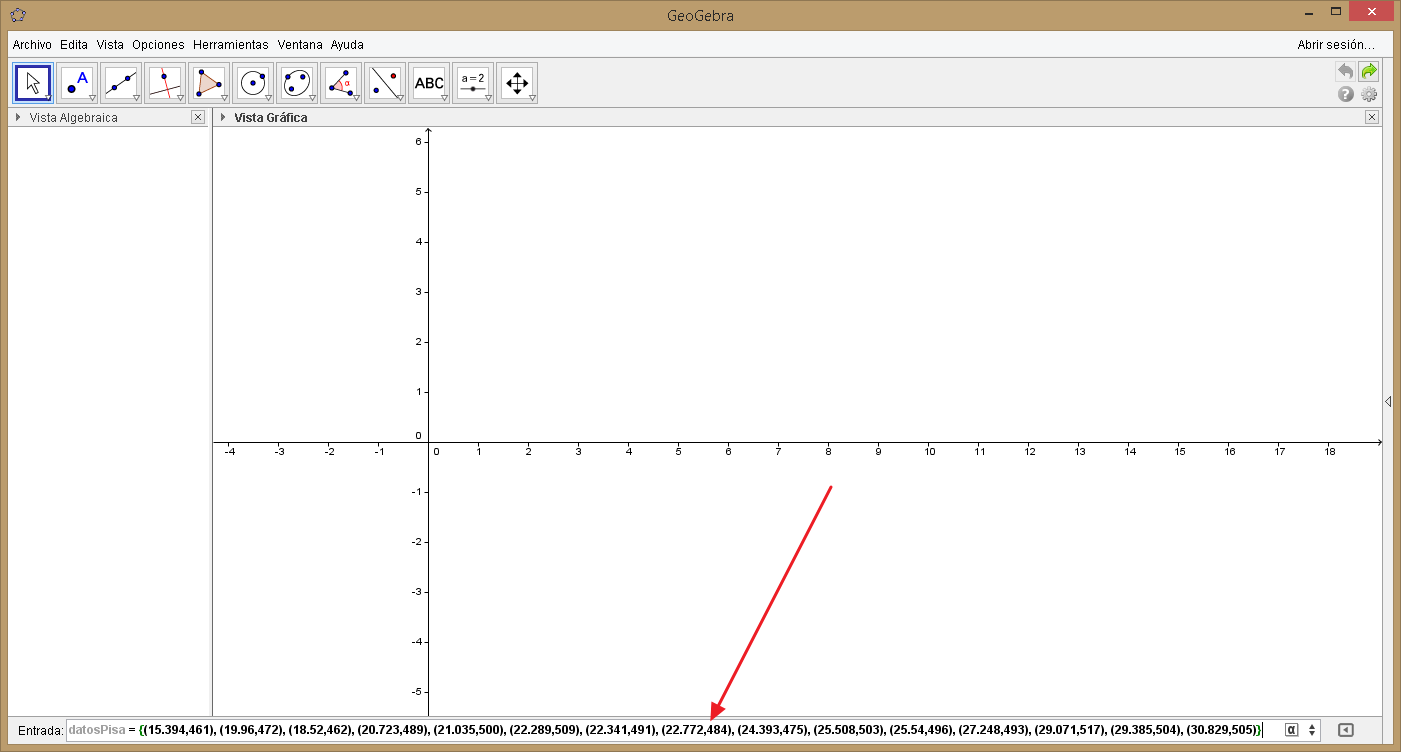
\includegraphics[width=16cm]{../fig/Tut10-11.png}
\end{center}
Cuando introduzcas estos datos en GeoGebra los verás aparecer en el panel de la izquierda, la {\em Vista Algebraica}, pero no en la {\em Vista gráfica}. Para hacerlos visibles tienes que pulsar sobre el botón circular situado a la izquierda de los datos en la {\em Vista Algebraica}, como muestra la figura:
\begin{center}
    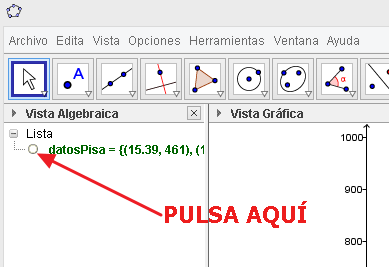
\includegraphics[width=8cm]{../fig/Tut10-12.png}
\end{center}
Después de hacer esto lo más probable es que todavía no veas los puntos. Para verlos,haz click con el botón derecho del ratón en algún lugar de la {\em Vista gráfica}, para hacer aparecer el menú contextual de ese panel, y selecciona {\em Mostrar todos los objetos}, como se ve en esta figura:
\begin{center}
    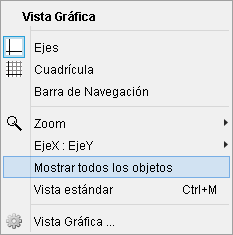
\includegraphics[width=5cm]{../fig/Tut10-13.png}
\end{center}
Al hacerlo verás aparecer la nube de puntos. Todavía es posible que tengas que hacer zoom o cambiar la escala de los ejes para llegar a una visualización que nos parezca satisfactoria. Por ejemplo, yo he modificado la posición y escala de los ejes, para que el punto de corte ocurra en el valor $400$ del eje vertical.
\begin{center}
    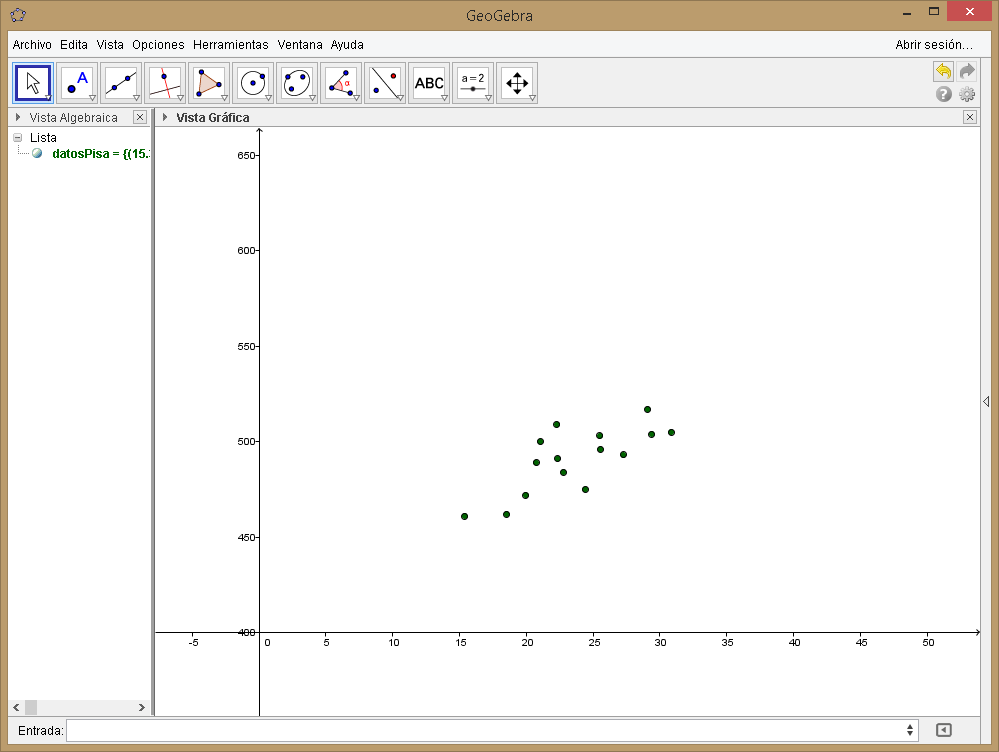
\includegraphics[width=11cm]{../fig/Tut10-14.png}
\end{center}
Puedes explorar el menú {\em Vista Gráfica} (identificado por la rueda dentada que aparece en el menú contextual que hemos usado antes), en el que puedes modificar estos y muchos otros parámetros de la visualización.

La limitación evidente de esta forma de trabajar es que en la mayoría de los casos partiremos de una tabla, o de un fichero csv con los datos. Por ejemplo, el fichero adjunto
\begin{center}
\fichero{../datos/Tut10-DatosPisaPais.csv}{Tut10-DatosPisaPais.csv},
\end{center}
cuyo contenido se muestra en la Figura \ref{tut10:fig:FicheroCsvPisaPais} contiene los mismos datos de este ejemplo, en un formato mucho más común en la práctica.
\begin{figure}[h!]
\begin{center}
    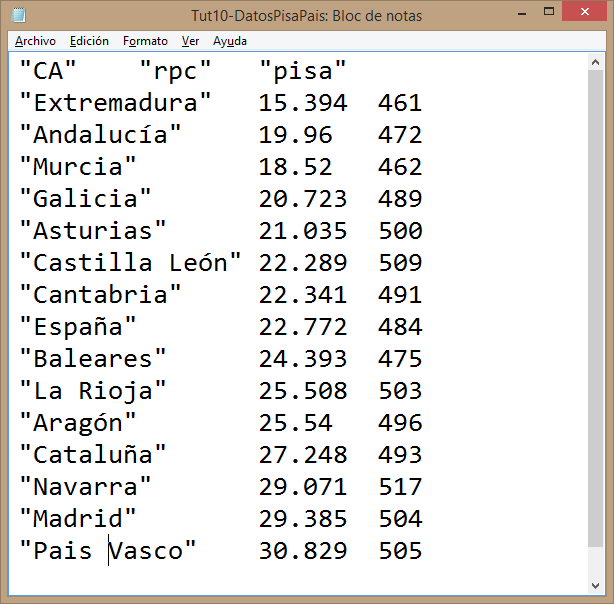
\includegraphics[width=8cm]{../fig/Tut10-01.png}
\end{center}
\caption{Fichero {\tt csv} con los datos del ejemplo sobre el estudio PISA.}
\label{tut10:fig:FicheroCsvPisaPais}
\end{figure}
Una posibilidad es usar la {\em Hoja de Cálculo} que incorpora GeoGebra, e importar el fichero {\tt csv} como hemos hecho en Calc. GeoGebra ofrece, en sus versiones recientes, muchas menos posibilidades de configuración de ese proceso de importación que, por ejemplo, Calc. Puedes encontrar más información en este enlace:
\begin{center}
\link{http://wiki.geogebra.org/en/Spreadsheet_View}{http://wiki.geogebra.org/en/Spreadsheet\_View}
\end{center}
Pero para trabajar cómodamente con ficheros de datos más complejos y, en general, para poder exprimir al máximo la información de estos datos,  es sensiblemente mejor recurrir a un programa especializado como R.

\subsection{En R.}
\label{tut10:subsec:DiagramaDispersionEnR}

Vamos a empezar con un ejemplo muy elemental de cómo se dibuja un diagrama de dispersión en R. Partimos de dos vectores de coordenadas:
% set.seed(2014)
\begin{knitrout}
\definecolor{shadecolor}{rgb}{0.969, 0.969, 0.969}\color{fgcolor}\begin{kframe}
\begin{alltt}
\hlstd{x} \hlkwb{=} \hlkwd{c}\hlstd{(}\hlnum{1}\hlstd{,} \hlnum{3}\hlstd{,} \hlnum{4}\hlstd{,} \hlnum{5}\hlstd{,} \hlnum{7}\hlstd{,} \hlnum{9}\hlstd{,} \hlnum{13}\hlstd{,} \hlnum{15}\hlstd{)}
\hlstd{y} \hlkwb{=} \hlkwd{c}\hlstd{(}\hlopt{-}\hlnum{0.888}\hlstd{,} \hlnum{3.12}\hlstd{,} \hlnum{4.27}\hlstd{,} \hlnum{5.6}\hlstd{,} \hlnum{8.06}\hlstd{,} \hlnum{12.2}\hlstd{,} \hlnum{15.9}\hlstd{,} \hlnum{17.2}\hlstd{)}
\end{alltt}
\end{kframe}
\end{knitrout}
Y para obtener el diagrama de dispersión basta con aplicar la función {\sf plot} así:
\begin{knitrout}
\definecolor{shadecolor}{rgb}{0.969, 0.969, 0.969}\color{fgcolor}\begin{kframe}
\begin{alltt}
\hlkwd{plot}\hlstd{(x, y)}
\end{alltt}
\end{kframe}
\includegraphics[width=\maxwidth]{figure/unnamed-chunk-2-1} 

\end{knitrout}
El diagrama resultante es, desde el punto de vista gráfico, muy básico. Pero, como sucede siempre en R, las posibilidades para modificar este gráfico, adaptándolo a nuestras necesidades y deseos, son casi ilimitadas. Más adelante en este tutorial vamos a adentrarnos, apenas unos pasos, en el universo de los gráficos con R.

Lo que hemos hecho para obtener ese gráfico es el esquema básico. En ejemplos más complicados y realistas, como hemos dicho, el punto de partida será a menudo un fichero de datos. Vamos a usar como ejemplo el fichero {\tt Tut10-DatosPisaPais.csv}, de datos del estudio PISA, que hemos incluido en la sección previa. Nuestro primer paso es leer los datos usando la función {\tt read.table}, que ya hemos usado en otras ocasiones para esto. Fíjate en que usamos la opción \verb#sep = "\t"#, porque las columnas de datos se han separado con tabuladores en el fichero {\tt csv}. ¿Cómo hemos sabido que se había usado el tabulador? Probando a leer los datos con el espacio como separador y descubriendo que se producía un error de lectura. Recuerda además que siempre es bueno comprobar que la lectura ha sido correcta, usando por ejemplo  la función {\tt head}:
{\small
\begin{knitrout}
\definecolor{shadecolor}{rgb}{0.969, 0.969, 0.969}\color{fgcolor}\begin{kframe}
\begin{alltt}
\hlstd{datosPisa} \hlkwb{=} \hlkwd{read.table}\hlstd{(}\hlkwc{file}\hlstd{=}\hlstr{"../datos/Tut10-DatosPisaPais.csv"}\hlstd{,} \hlkwc{header}\hlstd{=}\hlnum{TRUE}\hlstd{,} \hlkwc{sep} \hlstd{=} \hlstr{"\textbackslash{}t"}\hlstd{)}
\hlkwd{head}\hlstd{(datosPisa)}
\end{alltt}
\begin{verbatim}
##                     CA    rpc pisa
## 1          Extremadura 15.394  461
## 2     Andaluc\303\255a 19.960  472
## 3               Murcia 18.520  462
## 4              Galicia 20.723  489
## 5             Asturias 21.035  500
## 6 Castilla Le\303\263n 22.289  509
\end{verbatim}
\end{kframe}
\end{knitrout}
}
A partir de aquí, las cosas son sencillas. Usamos la notación habitual de los {\tt data.frmaes} de R para trabajar con las dos columnas que contienen los datos que vamos a representar y usamos la función {\tt plot} así:
\begin{knitrout}
\definecolor{shadecolor}{rgb}{0.969, 0.969, 0.969}\color{fgcolor}\begin{kframe}
\begin{alltt}
\hlkwd{plot}\hlstd{(datosPisa}\hlopt{$}\hlstd{rpc, datosPisa}\hlopt{$}\hlstd{pisa)}
\end{alltt}
\end{kframe}
\includegraphics[width=\maxwidth]{figure/unnamed-chunk-4-1} 

\end{knitrout}
Puedes probar también a usar
\begin{knitrout}
\definecolor{shadecolor}{rgb}{0.969, 0.969, 0.969}\color{fgcolor}\begin{kframe}
\begin{alltt}
\hlkwd{plot}\hlstd{(pisa} \hlopt{~} \hlstd{rpc,} \hlkwc{data}\hlstd{=datosPisa)}
\end{alltt}
\end{kframe}
\end{knitrout}
para ver que el resultado es el mismo. El símbolo \verb#~#, que ya ha aparecido en algún tutorial previo, es la forma de decir en R que estamos estudiando la relación entre esas dos variables.  En las próximas secciones volveremos a este ejemplo y seguiremos el análisis de regresión de esos datos. Pero antes, vamos a practicar en un ejercicio la lectura de datos a partir de
ficheros {\tt csv}.

\begin{ejercicio}
\label{tut10:ejercicio01}
En todos los casos se trata de leer un fichero {\tt csv} que contiene pares de datos, para
almacenar los valores de las variables $x$ e $y$ en sendos vectores de R, que llamaremos, claro está, {\tt x} e {\tt y}.  Antes de empezar, guarda los ficheros en la carpeta {\tt datos}  de tu directorio de trabajo, y recuerda que conviene echarle un vistazo al fichero de datos, usando un editor de texto (como el {\em Bloc de Notas} de Windows).
\begin{enumerate}
  \item El primer fichero es muy sencillo, no debe suponer
      problemas:\\
      \fichero{../datos/tut10-ejercicio01-1.csv}{tut10-ejercicio01-1.csv}
  \item Una variante del anterior, los mismos datos, con algunos cambios de formato:\\
      \fichero{../datos/tut10-ejercicio01-2.csv}{tut10-ejercicio01-2.csv}
  \item Y una tercera versión de los mismos datos:\\
      \fichero{../datos/tut10-ejercicio01-3.csv}{tut10-ejercicio01-3.csv}
\end{enumerate}
Soluciones en la página \pageref{tut10:ejercicio01:sol}.
\qed
\end{ejercicio}



\section{La recta de regresión lineal.}

\subsection{Interpolación en GeoGebra.}

Dado un conjunto de puntos, representados mediante su diagrama de dispersión, nuestro primer paso en la Sección \ref{curso-cap10:subsec:DiagramasDIspersionEleccionFuncionAdecuada} del libro (pág. \pageref{curso-cap10:subsec:DiagramasDIspersionEleccionFuncionAdecuada}) ha sido la búsqueda de una curva que pasara por todos y cada uno de los puntos del diagrama de dispersión. La técnica llamada {\em interpolación} permite construir una curva polinómica con esas propiedades. Para que puedas experimentar con esa idea hemos incluido un fichero GeoGebra:
\begin{center}
  \fichero{../ggb/Cap10-ExperimentoInterpolacion.ggb}{Cap10-ExperimentoInterpolacion.ggb}
\end{center}
que al abrirlo te mostrará esta imagen:
\begin{center}
    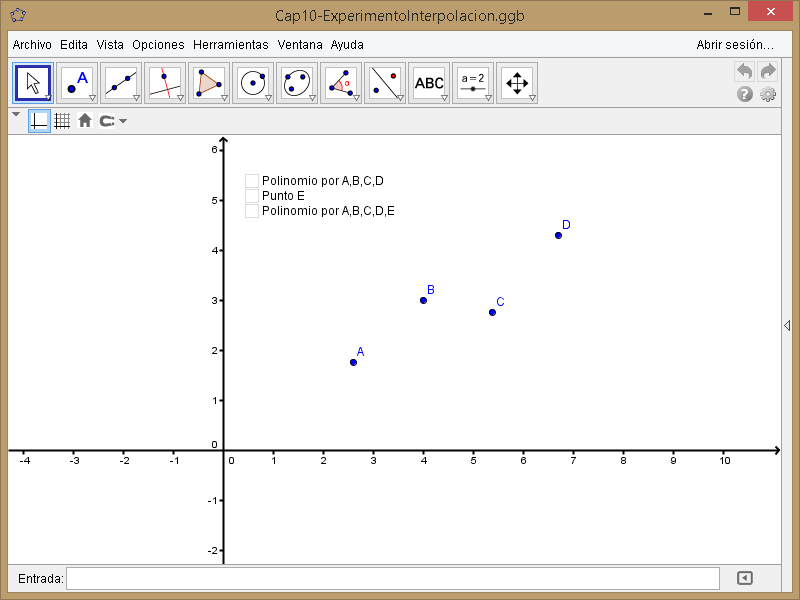
\includegraphics[width=14cm]{../fig/Tut10-15.png}
\end{center}
Empieza por marcar la casilla {\em Polinopmio por A, B, C, D} para ver aparecer la curva que pasa por esos puntos:
\begin{center}
    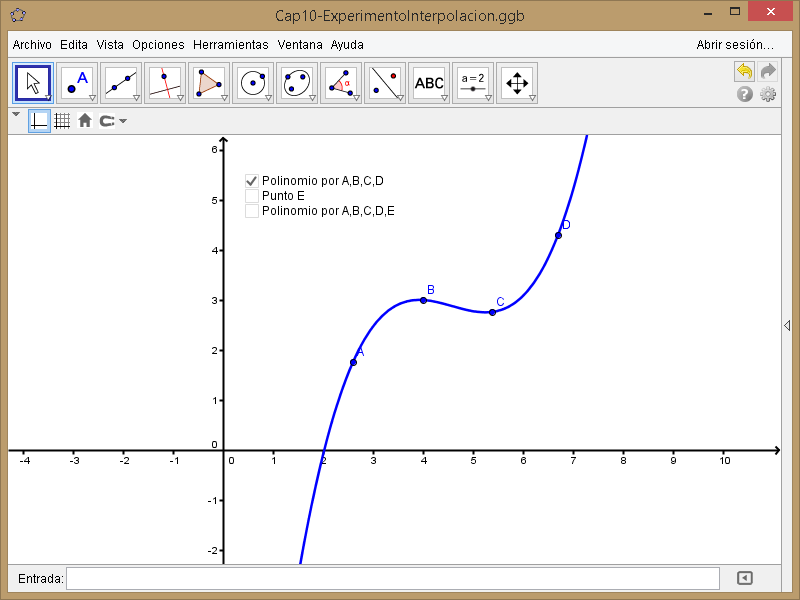
\includegraphics[width=14cm]{../fig/Tut10-16.png}
\end{center}
Si quieres, puedes probar a desplazar alguno de los puntos para ver cómo responde la curva. También puedes marcar la casilla para añadir un punto $E$ adicional que, si no has movido los puntos, inicialmente aparecerá cerca de la curva:
\begin{center}
    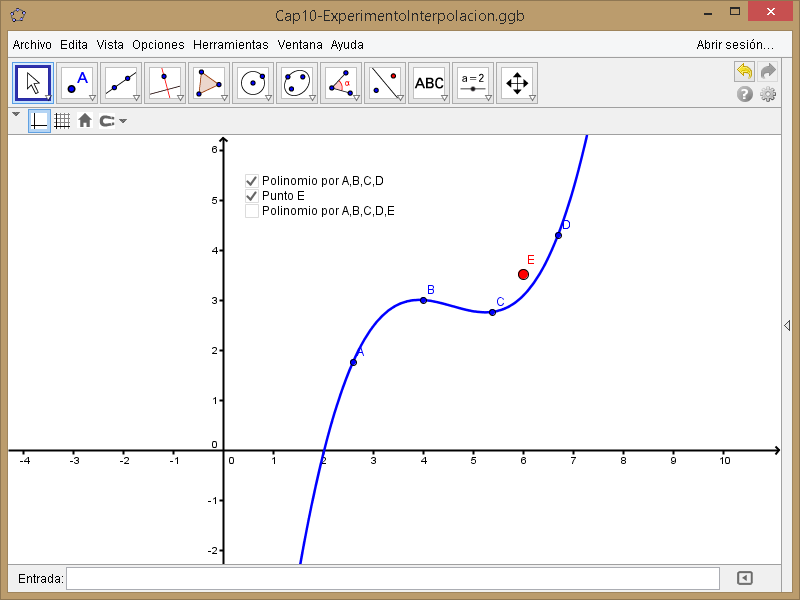
\includegraphics[width=15cm]{../fig/Tut10-17.png}
\end{center}
Finalmente, marca la casilla restante para mostrar la curva de interpolación que pasa por los cinco puntos y prueba a mover el punto $E$. Verás como incluso pequeñas modificaciones de la posición del punto pueden tener una influencia muy importante en la posición de esa curva.
\begin{center}
    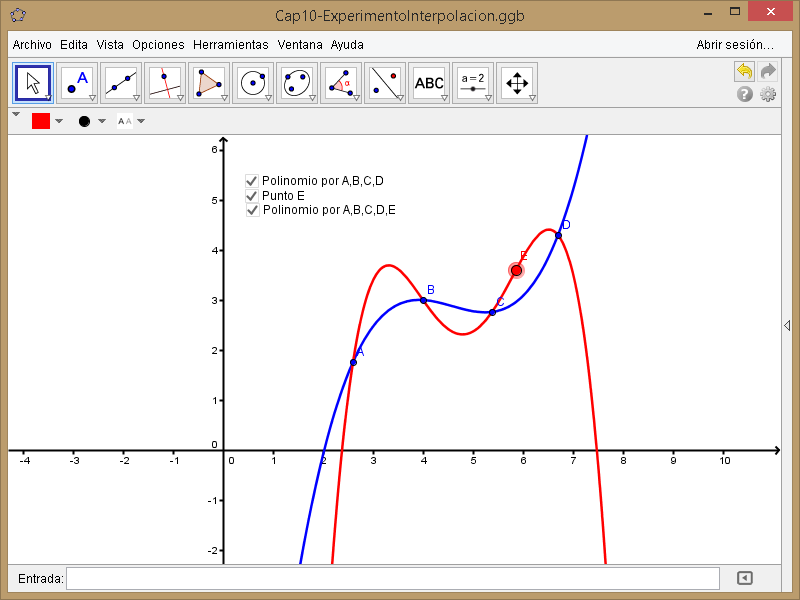
\includegraphics[width=15cm]{../fig/Tut10-18.png}
\end{center}
El  comando de GeoGebra  que nos permite construir la curva que pasa por los puntos $A, B, C$ y $D$ es:
{\tt   Polinomio[A, B, C, D]}.

\subsection{Recta de regresión en GeoGebra.}

El siguiente paso, como hemos discutido en el libro, es renunciar a buscar una curva que pase por todos los puntos. En su lugar buscamos la mejor recta posible para representar ese conjunto de puntos. En GeoGebra, la recta de regresión lineal se obtiene con la función {\tt AjusteLineal}, aplicada a una {\em lista} de puntos. Si todavía tienes abierto el fichero que hemos usado para la interpolación, puedes ejecutar este comando
  \begin{verbatim}
    AjusteLineal[{A, B, C, D}]
  \end{verbatim}
para obtener esa recta (si no usas las llaves el comando funcionará igualmente, GeoGebra las añade por ti). Y para los datos del estudio PISA que hemos usado al principio del tutorial, basta con hacer
\begin{verbatim}
AjusteLineal[datosPisa]
\end{verbatim}
para obtener la recta:
\begin{center}
    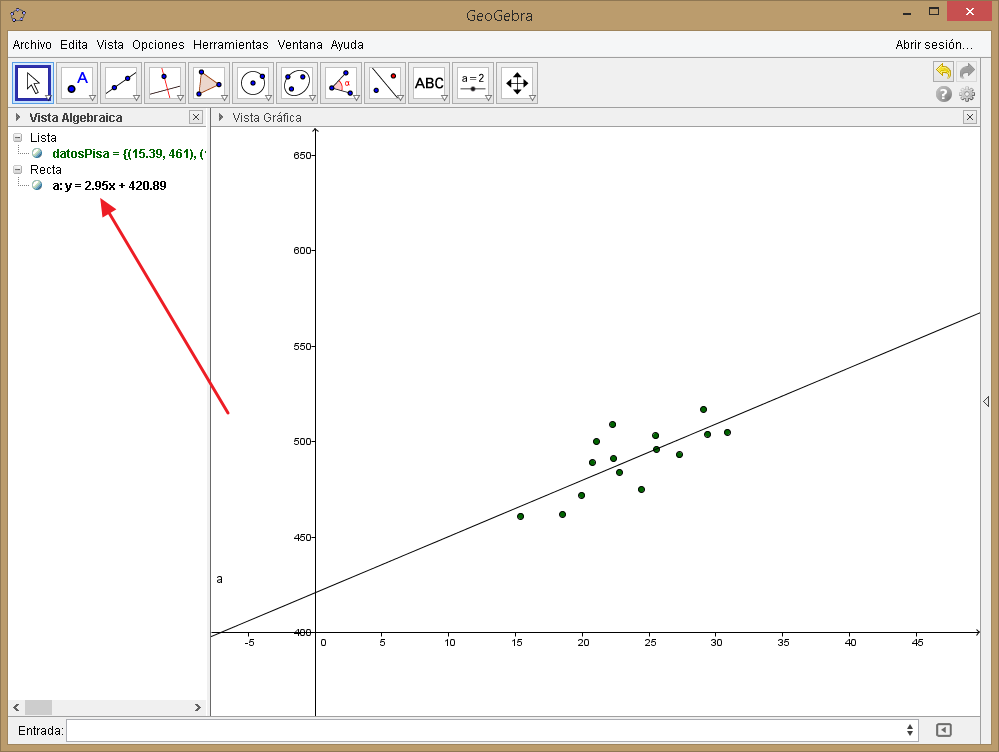
\includegraphics[width=15cm]{../fig/Tut10-19.png}
\end{center}
Hemos destacado la ecuación de la recta en la {\em Vista Algebraica} de GeoGebra, para que veas que ahí aparecen la pendiente y la ordenada en el origen.

\subsubsection*{Ficheros de GeoGebra para visualizar las ideas asociadas a la recta de regresión.}

Vamos a aprovechar este apartado para incluir aquí varios ficheros de GeoGebra que acompañan la discusión de la Sección \ref{curso-cap10:sec:RectaRegresionECCorrelacion} del libro (pág. \pageref{curso-cap10:sec:RectaRegresionECCorrelacion}). Para empezar, el fichero
\begin{center}
  \fichero{../ggb/Cap10-EcuacionRectaPendienteOrdenadaOrigen.ggb}{Cap10-EcuacionRectaPendienteOrdenadaOrigen.ggb}
\end{center}
permite refrescar el significado de la pendiente $b_1$ y la ordenada en el origen $b_0$ de una recta cuya ecuación es
\[y = b_0 + b_1 x,\]
usando un par de deslizadores como se ilustra en la figura
\begin{center}
    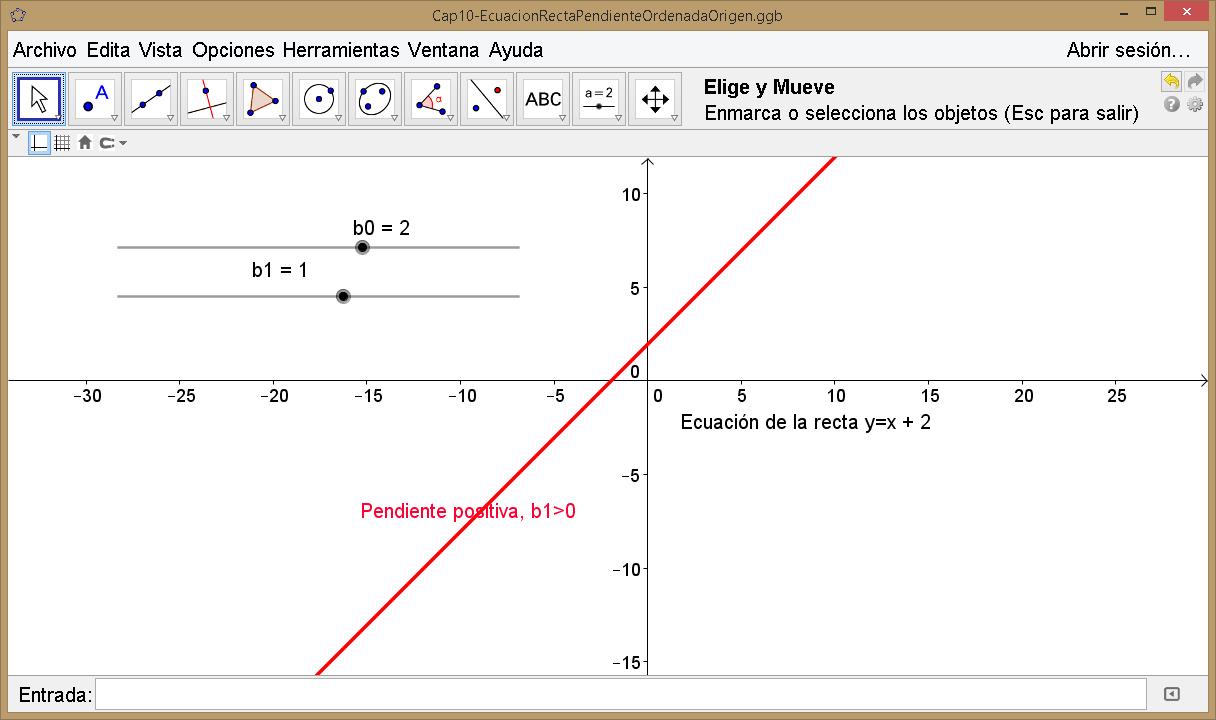
\includegraphics[width=15.5cm]{../fig/Tut10-20.png}
\end{center}
Prueba a mover esos deslizadores hasta asegurarte de que comprendes bien el efecto que cada uno de los coeficientes $b_0$ y $b_1$ tiene sobre la recta.

Una vez entendemos de las herramientas (los valores $b_0, b_1$) que nos van a permitir colocar la recta donde nosotros queramos, llega el momento de elegir la mejor recta para un conjunto dado de puntos. El fichero
\begin{center}
  \fichero{../ggb/Cap10-LaRectaDeRegresion.ggb}{Cap10-LaRectaDeRegresion.ggb}
\end{center}
te presenta una colección o nube de puntos (de color rojo) y te permite usar los puntos $M$ y $N$ para tratar de colocar la recta azul de la manera que consideres más representativa de la nube de puntos dada.
\begin{center}
    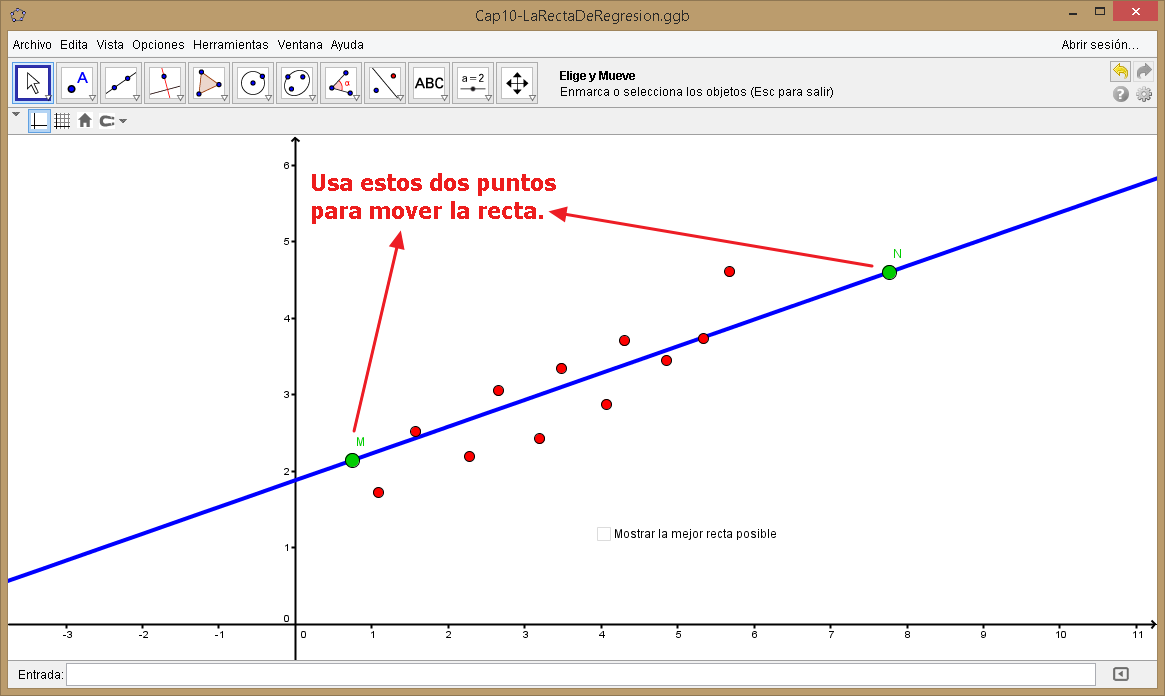
\includegraphics[width=15.5cm]{../fig/Tut10-21.png}
\end{center}
Una vez hecho esto, usa la casilla para mostrar la recta de regresión calculada por GeoGebra y comprobar si te has acercado a ese objetivo.

El siguiente paso consiste en cuantificar, para medirlo de forma precisa, el error que se comete al usar una recta como representante de la nube de puntos. El criterio que usamos es el error cuadrático, y el fichero Geogebra
\begin{center}
  \fichero{../ggb/Cap10-InterpretacionErrorCuadratico.ggb}{Cap10-InterpretacionErrorCuadratico.ggb}
\end{center}
trata de ilustrar la noción de error cuadrático. Como en el caso anterior, se muestra una nube de puntos y una recta que podemos tratar de colocar de la mejor manera posible. En este caso además de una casilla para mostrar la recta de regresión disponemos de otra que nos permite ver los cuadrados que determinan ese error {\em cuadrático}. Prueba a mover la recta hacia la posición que ocupa la recta de regresión y observa como la suma total de las áreas de esos cuadrados se reduce a un mínimo en esa posición.
\begin{center}
    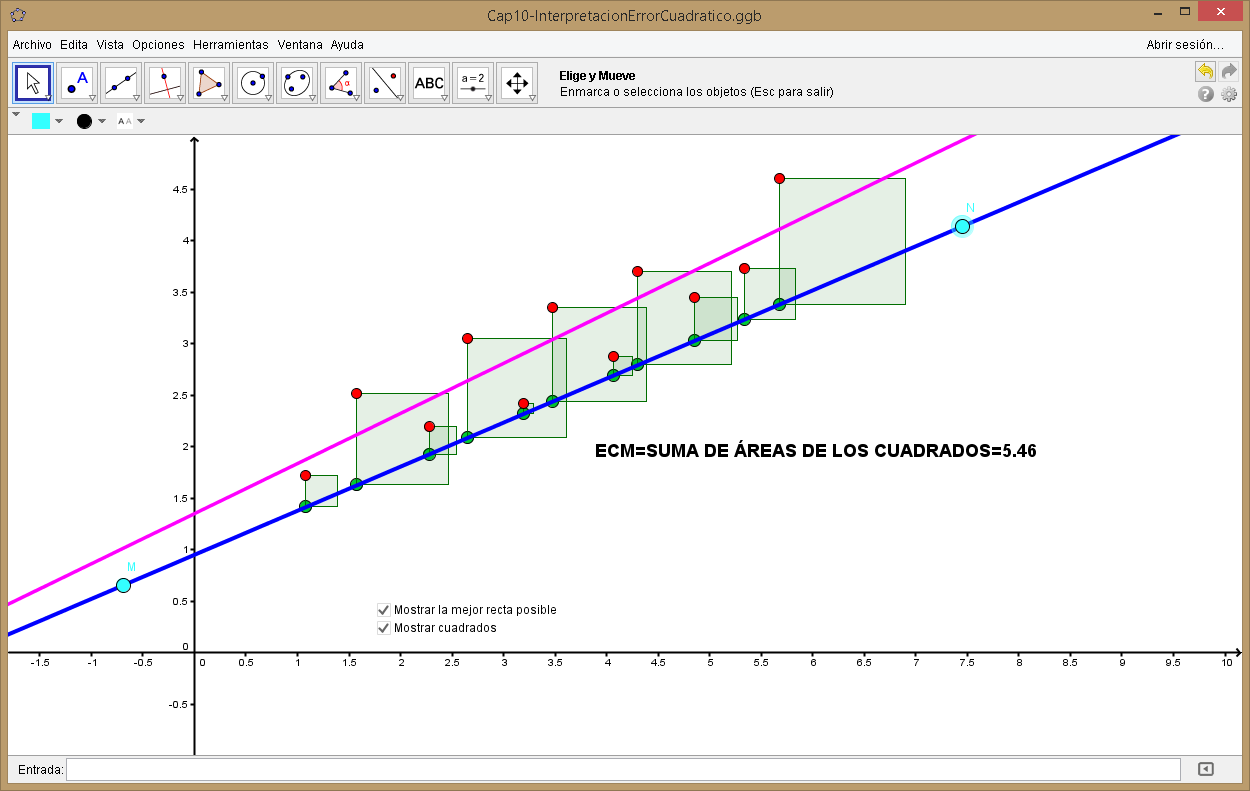
\includegraphics[width=15.6cm]{../fig/Tut10-22.png}
\end{center}
Cuando mueves la recta hasta hacerla coincidir exactamente con la recta de regresión, este fichero también permite visualizar los valores de los {\em residuos}, que son los segmentos verticales que conectan los puntos de la nube inicial de datos (los puntos rojos) con los puntos correspondientes de la recta de regresión (los puntos verdes).

Vamos a cerrar este apartado con dos ficheros GeoGebra, que permiten explorar las ideas que aparecen en las Figuras \ref{curso-cap10:fig:RectaTangenteParabola} y \ref{curso-cap10:fig:RectaComoAproximacionLocal} del libro (págs. \pageref{curso-cap10:fig:RectaTangenteParabola} y \pageref{curso-cap10:fig:RectaComoAproximacionLocal}, respectivamente). Los ficheros son:
\begin{center}
\fichero{../ggb/Cap10-ZoomEnParabola.ggb}{Cap10-ZoomEnParabola.ggb}\\
\fichero{../ggb/Cap10-RectasZoomHaciaFuera.ggb}{Cap10-RectasZoomHaciaFuera.ggb}
\end{center}
En ambos casos, se trata de hacer zoom en la figura, hacia dentro en la primera y hacia fuera en la segunda. Puedes usar la rueda del ratón o las teclas {\tt Ctrl +} y {\tt Ctrl -} para hacer esto.


\subsection{La recta de regresión en R.}

En esta sección vamos a comenzar el estudio de los comandos de R necesarios para el análisis de regresión lineal. Las posibilidades de R van mucho más lejos de lo que vamos a ver aquí, pero, como siempre, es necesario empezar por lo más básico.

Para empezar a trabajar vamos a usar los datos del informe PISA con los que abríamos este tutorial. Supondremos que los datos están disponibles en el {\tt data.frame} de R llamado {\tt datosPisa} que hemos creado en la Sección \ref{tut10:subsec:DiagramaDispersionEnR} (pág. \pageref{tut10:subsec:DiagramaDispersionEnR}). En primer lugar, vamos a ver como calcular la covarianza de estos dos vectores, cosa que es extremadamente fácil de hacer en R:
\begin{knitrout}
\definecolor{shadecolor}{rgb}{0.969, 0.969, 0.969}\color{fgcolor}\begin{kframe}
\begin{alltt}
\hlkwd{cov}\hlstd{(datosPisa}\hlopt{$}\hlstd{rpc, datosPisa}\hlopt{$}\hlstd{pisa)}
\end{alltt}
\begin{verbatim}
## [1] 55.261
\end{verbatim}
\end{kframe}
\end{knitrout}
Recuerda que en R {\bf se trata siempre de la covarianza muestral}, que usa $n-1$ en el denominador. Si
deseas la covarianza que usa $n$, debes usar el truco habitual, multiplicando por $n-1$ y dividendo por $n$.

Con la función {\tt cov} estamos listos para calcular la pendiente de la recta de regresión, que de
acuerdo con la Ecuación \ref{curso-cap10:ecu:RectaRegresionPendienteOrdenadaOrigen} (pág.
\pageref{curso-cap10:ecu:RectaRegresionPendienteOrdenadaOrigen}) del libro es:

\begin{knitrout}
\definecolor{shadecolor}{rgb}{0.969, 0.969, 0.969}\color{fgcolor}\begin{kframe}
\begin{alltt}
\hlstd{(b1} \hlkwb{=} \hlkwd{cov}\hlstd{(datosPisa}\hlopt{$}\hlstd{pisa, datosPisa}\hlopt{$}\hlstd{rpc)}\hlopt{/}\hlkwd{var}\hlstd{(datosPisa}\hlopt{$}\hlstd{rpc))}
\end{alltt}
\begin{verbatim}
## [1] 2.951
\end{verbatim}
\end{kframe}
\end{knitrout}
Y la ordenada en el origen es, entonces:

\begin{knitrout}
\definecolor{shadecolor}{rgb}{0.969, 0.969, 0.969}\color{fgcolor}\begin{kframe}
\begin{alltt}
\hlstd{(b0} \hlkwb{=} \hlkwd{mean}\hlstd{(datosPisa}\hlopt{$}\hlstd{pisa)} \hlopt{-} \hlstd{b1} \hlopt{*} \hlkwd{mean}\hlstd{(datosPisa}\hlopt{$}\hlstd{rpc))}
\end{alltt}
\begin{verbatim}
## [1] 420.89
\end{verbatim}
\end{kframe}
\end{knitrout}
Así que la recta de regresión es, aproximadamente,
\[y = 420.9 + 2.951\cdot x\]
Recuerda que ya habíamos obtenido esta recta en Geogebra, así que es un buen momento para que compruebes que el resultado es el mismo.

\subsubsection*{La función {\tt attach}.}

Si te has cansado de escribir todo el rato
\begin{center}
\verb#datosPisa$#,
\end{center}
puedes ejecutar
\begin{knitrout}
\definecolor{shadecolor}{rgb}{0.969, 0.969, 0.969}\color{fgcolor}\begin{kframe}
\begin{alltt}
  \hlkwd{attach}\hlstd{(datosPisa)}
\end{alltt}
\end{kframe}
\end{knitrout}
Cuando lo ejecutes puede que veas algún mensaje de advertencia de R. No te preocupes por el momento. Con este comando le decimos a R que queremos acceder a las variables de ese {\tt data.frame} sin necesidad de precederlas con \verb#datosPisa$#. Por ejemplo, en lugar de \verb#datosPisa$rpc# ahora puedes decir simplemente
\begin{knitrout}
\definecolor{shadecolor}{rgb}{0.969, 0.969, 0.969}\color{fgcolor}\begin{kframe}
\begin{alltt}
\hlstd{rpc}
\end{alltt}
\begin{verbatim}
##  [1] 15.394 19.960 18.520 20.723 21.035 22.289 22.341 22.772 24.393 25.508
## [11] 25.540 27.248 29.071 29.385 30.829
\end{verbatim}
\end{kframe}
\end{knitrout}
y, como ves, R lo entiende sin problemas. El problema de hacer esto es que en ocasiones se crean ambigüedades entre las variables del {\tt data.frame} y otras posibles variables. Especialmente en programas más complicados y cuando se trabaja con varios {\tt data.frames} a la vez. En un programa sencillo que escribimos para un cálculo corto, puede ser la solución más cómoda. Pero el uso generalizado de {\tt attach} no es una práctica muy recomendable y la mayoría de programadores expertos de R lo desaconsejan. Cuando aprendas un poco más de R podrás evitarlo casi siempre, mediante herramientas como la función {\tt with} y la opción {\tt data} de muchas funciones. Además, el uso del tabulador en RStudio aligera mucho el trabajo adicional que esto supone. Nosotros vamos a seguir adelante en el Tutorial sin usar {\tt attach}. La forma de deshacer sus efectos es mediante
\begin{knitrout}
\definecolor{shadecolor}{rgb}{0.969, 0.969, 0.969}\color{fgcolor}\begin{kframe}
\begin{alltt}
\hlkwd{detach}\hlstd{(datosPisa)}
\hlstd{rpc}
\end{alltt}


{\ttfamily\noindent\bfseries\color{errorcolor}{\#\# Error in eval(expr, envir, enclos): objeto 'rpc' no encontrado}}\end{kframe}
\end{knitrout}
y el mensaje de error nos confirma de que hemos vuelto a la situación previa al uso de {\tt attach}.

%tienes dos opciones:
%\begin{enumerate}
%  \item La más cómoda, pero que a la vez es la más peligrosa por el riesgo de errores que conlleva, es ejecutar (¡no lo hagas hasta seguir leyendo!)
%      <<eval=FALSE>>=
%      attach(datosPisa)
%      @
%      Con este comando le decimos a R que queremos acceder a las variables de ese {\tt data.frame} sin necesidad de precederlas con \verb#datosPisa$#. El problema de hacer esto es que en ocasiones se crean ambigüedades entre las variables del {\tt data.frame} y otras posibles variables. Especialmente en programas más complicados y cuando se trabaja con varios {\tt data.frames} a la vez. En un programa sencillo que escribimos para un cálculo corto, puede ser la solución más cómoda. Pero el uso generalizado de {\tt attach} no es una práctica muy recomendable y la mayoría de programadores expertos de R lo desaconsejan.
%
%  \item Por otro lado, puedes usar la función {\tt with} para crear una estructura que indica la sentencia (o sentencias, si ocupan varias líneas) de R en las que quieres usar las variables de un {\tt data.frame}. Por ejemplo, el cálculo de la pendiente y ordenada en el origen que hemos hecho antes quedaría así:
%      <<>>=
%      coefRecta = with(datosPisa, {
%        pendiente = cov(pisa, rpc)/var(rpc)
%        ordOrigen = mean(pisa) - pendiente * mean(rpc)
%        c(pendiente, ordOrigen)
%        })
%      coefRecta
%      (b1 = coefRecta[1])
%      (b0 = coefRecya[2])
%      @
%      Fíjate en que hemos añadido dos líneas para mostrar los resultados, porque los paréntesis que usamos habitualmente no funcionan correctamente dentro de la estructura {\tt with}.
%\end{enumerate}

\subsubsection*{Añadir la recta de regresión al diagrama de dispersión.}

Naturalmente, una vez calculada la recta de regresión, queremos verla incluida en el diagrama de dispersión. Para ello, disponemos de la función {\tt abline}, que puede dibujar cualquier recta. El nombre de esa función se debe a que tradicionalmente las rectas se han escrito así:
\[y = a + b \cdot x\]
a partir de su pendiente $b$ y ordenada en el origen $a$. Para usarlo en nuestro ejemplo hacemos:
y el resultado es la gráfica que se muestra en la Figura \ref{tut10:fig:RectaRegresionEnDiagramaDispersionPisaPais}.
\begin{figure}[h!]
\begin{center}
    %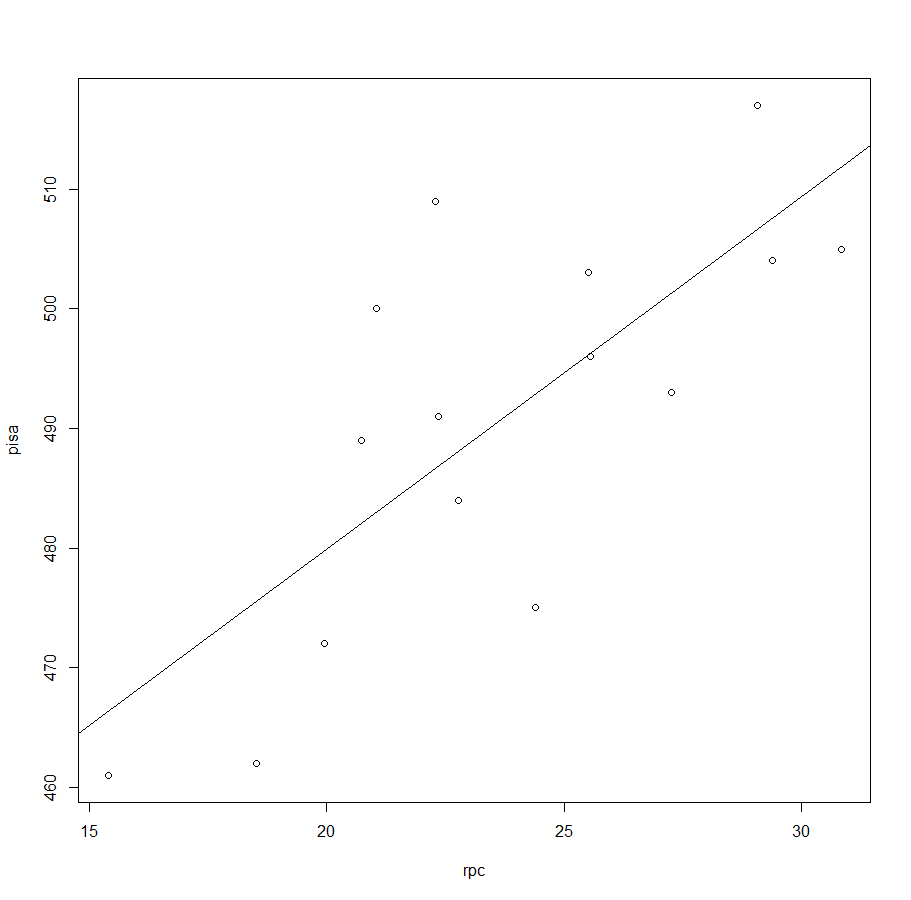
\includegraphics[width=12cm]{../fig/Tut10-04.png}
\begin{knitrout}
\definecolor{shadecolor}{rgb}{0.969, 0.969, 0.969}\color{fgcolor}\begin{kframe}
\begin{alltt}
    \hlkwd{plot}\hlstd{(datosPisa}\hlopt{$}\hlstd{pisa} \hlopt{~} \hlstd{datosPisa}\hlopt{$}\hlstd{rpc)}
    \hlkwd{abline}\hlstd{(}\hlkwc{a} \hlstd{= b0,} \hlkwc{b} \hlstd{= b1)}
\end{alltt}
\end{kframe}
\includegraphics[width=\maxwidth]{figure/unnamed-chunk-12-1} 

\end{knitrout}
\end{center}
\caption{Recta de regresión en el diagrama de dispersión para el Ejemplo de los datos del informe PISA.}
\label{tut10:fig:RectaRegresionEnDiagramaDispersionPisaPais}
\end{figure}

Está claro que, como hemos dicho antes, se trata de un gráfico muy sencillo, aunque suficiente para muchos de nuestros propósitos. Pronto aprenderemos a mejorarlo. Recuerda además que ya obtuvimos este gráfico con GeoGebra, así que es una buena idea que compares las dos versiones.



\subsection{Coeficiente de correlación, Residuos y error cuadrático medio}
\label{tut10:subsec:CoeficienteCorrelacionResiduosEC}

El coeficiente de correlación $r$ que aparece en la Ecuación
\ref{curso-cap10:ecu:CoeficienteRegresionPearson} (pág.
\pageref{curso-cap10:ecu:CoeficienteRegresionPearson}) del libro, se calcula en R con la función {\tt cor}. Así que, para los datos del estudio PISA  se obtiene
\begin{knitrout}
\definecolor{shadecolor}{rgb}{0.969, 0.969, 0.969}\color{fgcolor}\begin{kframe}
\begin{alltt}
\hlkwd{cor}\hlstd{(datosPisa}\hlopt{$}\hlstd{pisa, datosPisa}\hlopt{$}\hlstd{rpc)}
\end{alltt}
\begin{verbatim}
## [1] 0.75277
\end{verbatim}
\end{kframe}
\end{knitrout}

\begin{ejercicio}
\label{tut10:ejercicio02}
\begin{enumerate}
  \item[]
  \item Comprueba que el resultado de {\tt cor} es el mismo que cuando se usa {\tt cov} y la fórmula de la Ecuación \ref{curso-cap10:ecu:CoeficienteRegresionPearson} del libro (pág. \pageref{curso-cap10:ecu:CoeficienteRegresionPearson}). Recuerda que la función {\tt sd} sirve para calcular las cuasidesviaciones típicas que necesitarás para el denominador de esa fórmula.
  \item Averigua cuál es la función de GeoGebra que te permite calcular el coeficiente de correlación de la lista de puntos {\tt datosPisa} que hemos creado al principio del tutorial. Comprueba que el resultado es el mismo que hemos obtenido en R.
\end{enumerate}
Soluciones en la página \pageref{tut10:ejercicio02:sol}.
\qed
\end{ejercicio}



\subsubsection*{Residuos y error cuadrático medio}

Una vez que hemos obtenido la ecuación de la recta de regresión, también podemos usarla para calcular otros valores asociados al análisis de regresión como los residuos, o el error cuadrático, que son relevantes para el análisis de la varianza en el modelo de regresión. En la Sección \ref{tut10:sec:IntroduccionFuncionlm} de este tutorial vamos a aprender a usar la función {\tt lm} de R para hacer esta operación de una manera mucho más sencilla. Pero es bueno empezar por lo más básico, construyendo los resultados paso a paso.

Por ejemplo, para calcular los residuos con los datos del estudio PISA debemos primero calcular la diferencia entre los valores para las pruebas PISA que predice la recta, calculados a partir de {\tt rpc}, y los valores de {\tt pisa} que se han medido en la muestra. Para obtener los valores que predice la recta hacemos
{\small
\begin{knitrout}
\definecolor{shadecolor}{rgb}{0.969, 0.969, 0.969}\color{fgcolor}\begin{kframe}
\begin{alltt}
\hlstd{(pisaRecta} \hlkwb{=} \hlstd{b0} \hlopt{+} \hlstd{b1} \hlopt{*} \hlstd{datosPisa}\hlopt{$}\hlstd{rpc)}
\end{alltt}
\begin{verbatim}
##  [1] 466.32 479.79 475.54 482.05 482.97 486.67 486.82 488.09 492.88 496.17
## [11] 496.26 501.30 506.68 507.61 511.87
\end{verbatim}
\end{kframe}
\end{knitrout}
}
que, como se ve, da como resultado el vector de valores predichos ({\em fitted values}, en inglés). Ahora sólo tenemos que restar estos de {\tt pisa} para obtener los residuos:
{\small
\begin{knitrout}
\definecolor{shadecolor}{rgb}{0.969, 0.969, 0.969}\color{fgcolor}\begin{kframe}
\begin{alltt}
\hlstd{(residuos} \hlkwb{=} \hlstd{datosPisa}\hlopt{$}\hlstd{pisa} \hlopt{-} \hlstd{pisaRecta)}
\end{alltt}
\begin{verbatim}
##  [1]  -5.31931  -7.79347 -13.54407   6.95493  17.03423  22.33370   4.18025
##  [8]  -4.09162 -17.87515   6.83451  -0.25992  -8.30019  10.32018  -3.60643
## [15]  -6.86764
\end{verbatim}
\end{kframe}
\end{knitrout}
}
Si lo que queremos es el error cuadrático EC, basta con hacer la suma de los cuadrados de los residuos:
\begin{knitrout}
\definecolor{shadecolor}{rgb}{0.969, 0.969, 0.969}\color{fgcolor}\begin{kframe}
\begin{alltt}
\hlstd{(EC} \hlkwb{=} \hlkwd{sum}\hlstd{(residuos}\hlopt{^}\hlnum{2}\hlstd{))}
\end{alltt}
\begin{verbatim}
## [1] 1745.9
\end{verbatim}
\end{kframe}
\end{knitrout}
Como hemos dicho, en la Sección \ref{tut10:sec:IntroduccionFuncionlm} de
este tutorial veremos como se pueden obtener muchos de estos valores usando {\tt lm}. Pero antes, y para que puedas hacer fácilmente los siguientes ejercicios, vamos a incluir aquí un fichero de comandos R que sirve para realizar todos los pasos anteriores:

\begin{center}
\fichero{./code/Tut10-RectaRegresion.R}{Tut10-RectaRegresion.R}
\end{center}

\begin{ejercicio}
\label{tut10:ejercicio03}
Vamos a usar ese fichero de R para comprobar los valores que aparecen en algunos ejemplos del Capítulo \ref{curso-cap:RegresionLinealSimple}. Hemos incluido ficheros {\tt csv} para facilitarte las operaciones. En todos los casos, lo más recomendable es que repitas un análisis completo, ejecutando todos los comandos del fichero para cada conjunto de datos.
\begin{enumerate}
    \item Ejemplo \ref{curso-cap10:ejem:Regresion01} (pág \pageref{curso-cap10:ejem:Regresion01}). Datos en el fichero:\\
        \fichero{../datos/cap10-EjemploRegresion01.csv}{cap10-EjemploRegresion01.csv}

    \item Ejemplo \ref{curso-cap10:ejem:RectaMalaAproximacion01} (pág \pageref{curso-cap10:ejem:RectaMalaAproximacion01}). Datos en el fichero:\\
        \fichero{../datos/Cap10-EjemploRectaMalaAproximacion01.csv}{Cap10-EjemploRectaMalaAproximacion01.csv}.

    \item Ejemplo \ref{curso-cap10:ejem:RectaMalaAproximacion02} (pág \pageref{curso-cap10:ejem:RectaMalaAproximacion02}). Datos en el fichero:\\
        \fichero{../datos/Cap10-EjemploRectaMalaAproximacion02.csv}{Cap10-EjemploRectaMalaAproximacion02.csv}.

    \item Ejemplo \ref{curso-cap10:ejem:Anova01} (pág \pageref{curso-cap10:ejem:Anova01}).\\
        Primero los puntos ``no ruidosos''.  Datos en el fichero:\\
        \fichero{../datos/Cap10-Ejemplo-Anova01.csv}{Cap10-Ejemplo-Anova01.csv}.

    \item Y del mismo ejemplo \ref{curso-cap10:ejem:Anova01},
        ahora los puntos ``ruidosos''.  Datos en el fichero:\\
        \fichero{../datos/Cap10-Ejemplo-Anova02.csv}{Cap10-Ejemplo-Anova02.csv}.
\end{enumerate}
\qed
\end{ejercicio}


\subsection{Un gráfico de regresión más expresivo}
\label{tut10:subsec:MejorandoGraficosR}

\noindent{\bf Opcional:
esta sección puede omitirse en una primera lectura. }

El gráfico de regresión que hemos mostrado en la Figura es bastante elemental, incluso rudimentario. Aquí vamos a ver algunos comandos y opciones de R que ayudan a conseguir un resultado visualmente más atractivo. Puedes considerar esta sección como una invitación a explorar más en las (muy amplias) capacidades gráficas de R, de las que aquí sólo mostramos una ínfima parte.

Para empezar, hemos cambiado el comando
\begin{knitrout}
\definecolor{shadecolor}{rgb}{0.969, 0.969, 0.969}\color{fgcolor}\begin{kframe}
\begin{alltt}
\hlkwd{plot}\hlstd{(datosPisa}\hlopt{$}\hlstd{rpc, datosPisa}\hlopt{$}\hlstd{pisa)}
\end{alltt}
\end{kframe}
\end{knitrout}
por una versión más detallada.  Ocupa varias líneas que, como siempre en estos casos, deben ejecutarse conjuntamente:
{\small
\begin{knitrout}
\definecolor{shadecolor}{rgb}{0.969, 0.969, 0.969}\color{fgcolor}\begin{kframe}
\begin{alltt}
\hlkwd{plot}\hlstd{(datosPisa}\hlopt{$}\hlstd{rpc, datosPisa}\hlopt{$}\hlstd{pisa,}
    \hlkwc{lwd}\hlstd{=}\hlnum{2}\hlstd{,} \hlkwc{col}\hlstd{=}\hlstr{"red"}\hlstd{,} \hlkwc{cex}\hlstd{=}\hlnum{1.1}\hlstd{,} \hlkwc{cex.lab}\hlstd{=}\hlnum{1.1}\hlstd{,} \hlkwc{cex.axis}\hlstd{=}\hlnum{1.1}\hlstd{,} \hlkwc{bty}\hlstd{=}\hlstr{"n"}\hlstd{,}
    \hlkwc{xlab}\hlstd{=}\hlstr{"Renta per capita, a<U+00F1>o 2012, en miles de euros"}\hlstd{,}
    \hlkwc{ylab}\hlstd{=}\hlstr{"Puntos PISA2012 en Matem<U+00E1>ticas"}\hlstd{)}
\end{alltt}
\end{kframe}
\end{knitrout}
}
y que produce el resultado que aparece en la Figura \ref{tut10:fig:DiagramaDispersionPisaPaisMejora01}.
\begin{figure}[htb]
\begin{center}
%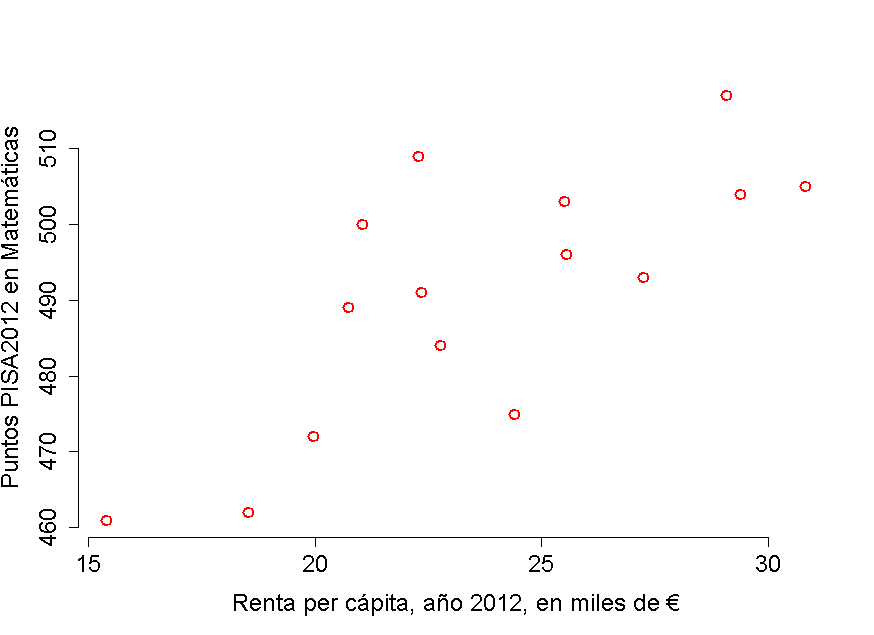
\includegraphics[width=13cm]{../fig/Tut10-05.png}
\begin{knitrout}
\definecolor{shadecolor}{rgb}{0.969, 0.969, 0.969}\color{fgcolor}
\includegraphics[width=\maxwidth]{figure/unnamed-chunk-18-1} 

\end{knitrout}
\end{center}
\caption{Primer paso para obtener un diagrama de dispersión mejorado para el ejemplo de los datos PISA.}
\label{tut10:fig:DiagramaDispersionPisaPaisMejora01}
\end{figure}
Vamos a comentar las modificaciones que hemos hecho:
\begin{itemize}
  \item La opción {\tt lwd=2} sirve para que los puntos $(x_i,y_i)$ se dibujen con un trazo más grueso (de hecho, {\tt lwd} proviene de {\em line width}, grosor de la línea).
  \item La opción {\verb#col="red"#} ya ha aparecido antes en los tutoriales, y sirve para cambiar el color de los símbolos que usa R, en este caso para que los puntos $(x_i,y_i)$ sean de color rojo.
  \item Las opciones que empiezan por {\tt cex} se refieren al tamaño de fuentes tipográficas y de algunos símbolos empleados en el gráfico. El nombre {\tt cex} proviene de {\em character expansion}, y su valor es un factor multiplicativo que nos indica cuántas veces más grande es el tipo de fuente que se usa, tomando como referencia el tipo base por defecto que usaría R. Así pues, {\tt cex=1.5} significa un símbolo 1.5 veces más grande que el valor por defecto, etc. Las variantes de {\tt cex} que aparecen se refieren a distintas partes del gráfico. Así, por ejemplo, {\tt cex.lab} se refiere al tamaño del texto en las frases que se usan como etiquetas de los ejes (en inglés {\em labels}, de ahí el nombre). En cambio {\tt cex.axis} se refiere a los números que aparecen en las escalas de los ejes (en inglés, {\em axis}).
  \item La opción \verb#bty="n"# (de {\em box type}, tipo de caja) sirve para decirle a R el tipo de marco que queremos que dibuje alrededor del gráfico. En este caso hemos optado por {\tt n}, de {\em none}, ninguno, porque vamos a añadirlo después.
  \item  Finalmente, los argumentos {\tt xlab} e {\tt ylab} sirven para añadir las etiquetas (de nuevo, {\em labels}) o frases que acompañan al eje $x$ y al eje $y$, respectivamente.
\end{itemize}

\begin{ejercicio}
\label{tut10:ejercicio04}
%\label{tut10:ejercicio03}
\begin{enumerate}
  \item[]
  \item Prueba a usar la opción {\tt main} para añadir un título general al gráfico.
  \item ¿Qué opción usarías para cambiar el tamaño de ese título?
  \item Prueba a añadir la opción {\tt pch=18}. ¿Qué ha cambiado? Busca información sobre los posibles valores de {\tt pch} (por ejemplo pidiéndole a R que ejecute {\tt ?pch}).
\end{enumerate}
\end{ejercicio}
\qed

A continuación vamos a rotular cada punto del gráfico con el nombre de la región a la que corresponde. Esos nombres están disponibles en la primera columna del {\tt data.frame datosPisa}. Para usarlos, ejecutamos este código
%\begin{verbatim}
%namesPisa=c("Extremadura","Andalucía","Murcia","Galicia","Asturias","CastillaLeón",
%            "Cantabria","ESPAÑA","Baleares","La Rioja","Aragón","Cataluña",
%            "Navarra","Madrid","País Vasco")
%\end{verbatim}
%Y luego hemos ejecutado el siguiente código
, que enseguida comentaremos:
\begin{knitrout}
\definecolor{shadecolor}{rgb}{0.969, 0.969, 0.969}\color{fgcolor}\begin{kframe}
\begin{alltt}
\hlkwd{par}\hlstd{(}\hlkwc{xpd}\hlstd{=}\hlnum{TRUE}\hlstd{)}
\hlkwd{text}\hlstd{(datosPisa}\hlopt{$}\hlstd{rpc, datosPisa}\hlopt{$}\hlstd{pisa,} \hlkwc{labels}\hlstd{=datosPisa}\hlopt{$}\hlstd{CA,}
    \hlkwc{pos}\hlstd{=}\hlnum{3}\hlstd{,} \hlkwc{offset}\hlstd{=}\hlnum{0.6}\hlstd{,}\hlkwc{font}\hlstd{=}\hlnum{3}\hlstd{)}
\hlkwd{par}\hlstd{(}\hlkwc{xpd}\hlstd{=}\hlnum{FALSE}\hlstd{)}
\end{alltt}
\end{kframe}
\end{knitrout}
Vamos a empezar por el comando {\tt text}. Este comando sirve para colocar texto en cualquier posición del gráfico que estamos dibujando. Como de costumbre, podemos utilizar vectores como argumentos. Así que en la opción {\tt labels} usamos el vector {\tt namesPisa} que contiene las etiquetas que queremos colocar junto a cada punto del gráfico. Los dos primeros argumentos de {\tt text} son dos vectores, con las coordenadas $x$ e $y$, respectivamente, de los puntos en los que se coloca cada una de esas etiquetas; en nuestro caso, se trata de los vectores {\tt rpc} y {\tt pisa}.  El argumento {\tt pos} (de {\em position}) sirve para colocar el texto debajo, a la izquierda, encima o a la derecha del punto, según que {\tt pos} valga 1, 2, 3 o 4. La opción {\tt offset} controla la separación entre el punto y el texto. Por último, la opción {\tt font} permite elegir entre un tipo normal (1), negrita (2), itálica (3) o negrita itálica (4).

¿Para qué sirve el comando {\tt par(xpd=TRUE)}? La función {\tt par} (de {\em parameter}, parámetro) es una de las funciones más importantes cuando se trata de modificar un gráfico de R. En este caso la usamos porque algunos de los nombres del vector {\tt namesPisa} son demasiado largos, y R ``recorta'' esos textos de las etiquetas para que no sobresalgan del marco del gráfico. Nosotros preferimos que los textos se muestren completos, aunque sobresalgan un poco, así que hemos usado la opción {\tt xpd=FALSE} que le dice a R que no haga ese recorte. Una vez colocadas las etiquetas volvemos a activar esa opción con {\tt par(xpd=FALSE)}. El resultado de estas operaciones es el gráfico de la Figura \ref{tut10:fig:DiagramaDispersionPisaPaisMejora02}.

\begin{figure}[htb]
\begin{center}
\begin{knitrout}
\definecolor{shadecolor}{rgb}{0.969, 0.969, 0.969}\color{fgcolor}
\includegraphics[width=\maxwidth]{figure/tut10_DiagramaDispersionPisaPaisMejora03-1} 

\end{knitrout}
\end{center}
\caption{Segundo paso para obtener un diagrama de dispersión mejorado.  }
\label{tut10:fig:DiagramaDispersionPisaPaisMejora02}
\end{figure}
A continuación añadimos la recta con
\begin{knitrout}
\definecolor{shadecolor}{rgb}{0.969, 0.969, 0.969}\color{fgcolor}\begin{kframe}
\begin{alltt}
\hlkwd{abline}\hlstd{(b0, b1,} \hlkwc{lwd}\hlstd{=}\hlnum{3}\hlstd{,} \hlkwc{col}\hlstd{=}\hlstr{"blue"}\hlstd{)}
\end{alltt}
\end{kframe}
\end{knitrout}
Las únicas modificaciones que hemos hecho son sobre el grosor y color del trazo. Ahora, para hacer visible la idea de residuo, vamos a añadir unos segmentos que conecten cada punto $(x_i,y_i)$ de la muestra con el correspondiente punto de la recta, que es $(x_i,\hat y_i)$. Para eso usamos el comando:
\begin{knitrout}
\definecolor{shadecolor}{rgb}{0.969, 0.969, 0.969}\color{fgcolor}\begin{kframe}
\begin{alltt}
\hlkwd{segments}\hlstd{(datosPisa}\hlopt{$}\hlstd{rpc, pisaRecta, datosPisa}\hlopt{$}\hlstd{rpc, datosPisa}\hlopt{$}\hlstd{pisa,}
     \hlkwc{lty}\hlstd{=}\hlnum{2}\hlstd{,}\hlkwc{lwd}\hlstd{=}\hlnum{3}\hlstd{)}
\end{alltt}
\end{kframe}
\end{knitrout}
cuyos dos primeros argumentos son las coordenadas $x$ e $y$ de los puntos iniciales de los segmentos, y cuyos argumentos tercero y cuarto son las coordenadas de los puntos finales de los segmentos. Fíjate en que los valores $\hat y_i$ están en el vector {\tt pisaRecta} que hemos calculando antes. Hemos ajustado además el grosor de la línea con {\tt lwd}, y el tipo de trazo, para que sea discontinuo, mediante la opción {\tt lty} (de {\em line type}).

\begin{ejercicio}
\label{tut10:ejercicio04}
Busca qué otros tipos de trazo puedes usar con distintos valores de {\tt lty}.
\end{ejercicio}
\qed

Como última modificación hemos dibujado un marco o ``caja'' alrededor del gráfico, usando el comando
\begin{knitrout}
\definecolor{shadecolor}{rgb}{0.969, 0.969, 0.969}\color{fgcolor}\begin{kframe}
\begin{alltt}
\hlkwd{box}\hlstd{(}\hlkwc{lwd}\hlstd{=}\hlnum{3}\hlstd{,}\hlkwc{bty}\hlstd{=}\hlstr{"l"}\hlstd{)}
\end{alltt}
\end{kframe}
\end{knitrout}
La opción {\tt bty} (de {\em box type}, tipo de caja), le indica a R como queremos que sea la forma del marco. Los códigos que se usan en este caso, son curiosos: se usa una letra, cuya forma indica la de la caja. Por ejemplo con \verb#bty="o"# le indicamos a R que queremos una caja con cuatro lados (la letra o es un círculo completo , mientras que con \verb#bty="u"# indicamos una caja a la que le falta el lado de arriba. Ya vimos antes que la opción "n" suprime la caja. Las otras opciones disponibles son:\\
\verb#"l", "7", "c", "u", "[", "]" #
\begin{ejercicio}
\label{tut10:ejercicio05}
Pruébalas todas para ver el efecto que producen.
\qed
\end{ejercicio}

El resultado final es el gráfico de la Figura \ref{tut10:fig:DiagramaDispersionPisaPaisMejora03}.
\begin{figure}[htb]
\begin{center}
%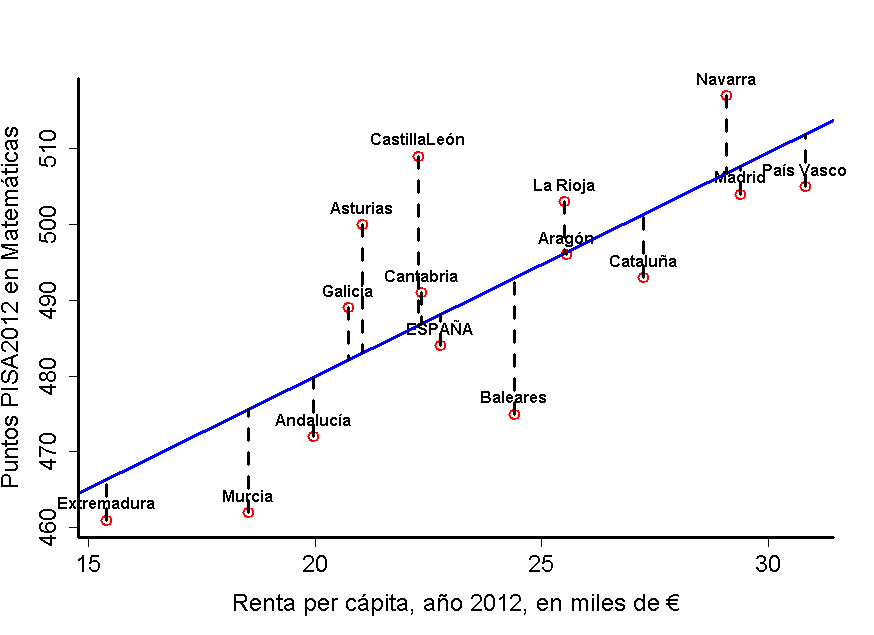
\includegraphics[width=15cm]{../fig/Tut10-07.png}
\begin{knitrout}
\definecolor{shadecolor}{rgb}{0.969, 0.969, 0.969}\color{fgcolor}
\includegraphics[width=\maxwidth]{figure/tut10_DiagramaDispersionPisaPaisMejora07-1} 

\end{knitrout}
\end{center}
\caption{El  diagrama de dispersión mejorado para el Ejemplo \ref{tut10:ejem:DatosPisaPais}.}
\label{tut10:fig:DiagramaDispersionPisaPaisMejora03}
\end{figure}
Como hemos dicho, hay mucho más que aprender sobre los gráficos de R, y aquí apenas hemos esbozado algunas ideas básicas. El lector interesado encontrará mucha información en la red, y en la abundante bibliografía, de la que citamos como ejemplo el libro (¡de más de 400 páginas!) {\em R Graphics Cookbook}, de Winston Chang, editado por O'Reilly (ISBN: 978-1-449-31695-2).


\section{Introducción a la función {\tt lm} de R}
\label{tut10:sec:IntroduccionFuncionlm}

\noindent{\bf Opcional:
esta sección puede omitirse en una primera lectura. Pero su contenido es muy importante para seguir avanzando en el aprendizaje de R.}

La función {\tt lm}, de {\em linear model} (modelo lineal) es, sin exageración alguna, una de las funciones más importantes de R. Una de las tareas más importantes de la Estadística y el Análisis de Datos es precisamente la construcción de modelos para describir la relación entre variables. Y, dentro de los posibles modelos, la familia de modelos lineales es la más importante. Esos modelos lineales se construyen en R usando la función {\tt lm}, así que podemos decir que esta función abre la puerta a algunas de las posibilidades más avanzadas del uso de R para la modelización estadística.

Pero empecemos por el modelo más sencillo, el modelo de regresión lineal simple que hemos descrito en el Capítulo \ref{curso-cap:RegresionLinealSimple}. Vamos a usar como ejemplo los puntos con ``ruido'' del Ejemplo \ref{curso-cap10:ejem:Anova01} del libro (pág. \pageref{curso-cap10:ejem:Anova01}), que tienes en el fichero {\tt csv} llamada {\tt Cap10-Ejemplo-Anova02.csv}, que ya hemos usado antes en los ejercicios de la página \pageref{tut10:ejercicio03} de este tutorial. De hecho, puedes usar los resultados del ejercicio $5$ de esa página para  compararlos con los que obtendremos aquí.

Empezamos leyendo los puntos de la muestra contenidos en ese fichero:
\begin{knitrout}
\definecolor{shadecolor}{rgb}{0.969, 0.969, 0.969}\color{fgcolor}\begin{kframe}
\begin{alltt}
\hlstd{datos} \hlkwb{=} \hlkwd{read.table}\hlstd{(}\hlstr{"../datos/Cap10-Ejemplo-Anova02.csv"}\hlstd{,} \hlkwc{header}\hlstd{=}\hlnum{TRUE}\hlstd{)}
\end{alltt}
\end{kframe}
\end{knitrout}
A continuación para explicarle a R que queremos usar el modelo de regresión lineal correspondiente a esos datos basta con ejecutar este comando:
\begin{knitrout}
\definecolor{shadecolor}{rgb}{0.969, 0.969, 0.969}\color{fgcolor}\begin{kframe}
\begin{alltt}
\hlstd{(lmXY} \hlkwb{=} \hlkwd{lm}\hlstd{(y} \hlopt{~} \hlstd{x,} \hlkwc{data}\hlstd{=datos))}
\end{alltt}
\begin{verbatim}
## 
## Call:
## lm(formula = y ~ x, data = datos)
## 
## Coefficients:
## (Intercept)            x  
##       0.983       -0.481
\end{verbatim}
\end{kframe}
\end{knitrout}
La sintaxis {\tt y ~ x} es la forma que tiene R de expresar que {\tt x} es la variable explicativa, e {\tt y} la variable respuesta en este modelo. Hemos almacenado el modelo en la variable {\tt lmXY} (el nombre podría ser cualquier otro) porque así será más fácil acceder a las propiedades de este modelo, como vamos a ver enseguida. La salida de este comando contiene, bajo el nombre {\tt coefficients}, los valores de $b_0$ y $b_1$. Concretamente, el valor de $b_1$, la pendiente, aparece bajo {\tt x}, porque $b_0$ es el coeficiente que acompaña a la $x$ en la ecuación
\[y = b_0 + b_1 \cdot x\]
de la recta. El valor de $b_0$ aparece bajo {\tt (Intercept)} porque ese es el nombre que se le da, en inglés, a la ordenada en el origen.

A primera vista, parece que no hemos ganado gran cosa, aparte de una forma rápida de llegar a los coeficientes de la recta. Pero en realidad el modelo, creado mediante {\tt lm}, tiene asociadas
muchas propiedades. Para ver algunas de ellas utiliza este comando:
\begin{knitrout}
\definecolor{shadecolor}{rgb}{0.969, 0.969, 0.969}\color{fgcolor}\begin{kframe}
\begin{alltt}
\hlkwd{summary}\hlstd{(lmXY)}
\end{alltt}
\begin{verbatim}
## 
## Call:
## lm(formula = y ~ x, data = datos)
## 
## Residuals:
##      Min       1Q   Median       3Q      Max 
## -0.01363 -0.01164 -0.00158  0.00744  0.02287 
## 
## Coefficients:
##             Estimate Std. Error t value Pr(>|t|)    
## (Intercept)   0.9828     0.0160    61.6  5.4e-12 ***
## x            -0.4808     0.0208   -23.1  1.3e-08 ***
## ---
## Signif. codes:  0 '***' 0.001 '**' 0.01 '*' 0.05 '.' 0.1 ' ' 1
## 
## Residual standard error: 0.0138 on 8 degrees of freedom
## Multiple R-squared:  0.985,	Adjusted R-squared:  0.983 
## F-statistic:  536 on 1 and 8 DF,  p-value: 1.29e-08
\end{verbatim}
\end{kframe}
\end{knitrout}
Como ves, R ha calculado muchas más propiedades de las que parecía. De hecho, insistimos, al usar {\tt summary} sólo estamos viendo una parte de las propiedades disponibles.

La ventaja de haber guardado el modelo en la variable {\tt lmXY} es que ahora podemos usar la notación con \verb#lmXY$# para acceder a esas propiedades. Prueba a escribir precisamente eso, \verb#lmXY$# en RStudio, y pulsa el tabulador. Aparecerá una lista de posibilidades, de la que vamos a ver el valor de la primera opción que R nos ofrece:
\begin{knitrout}
\definecolor{shadecolor}{rgb}{0.969, 0.969, 0.969}\color{fgcolor}\begin{kframe}
\begin{alltt}
\hlstd{lmXY}\hlopt{$}\hlstd{coefficients}
\end{alltt}
\begin{verbatim}
## (Intercept)           x 
##     0.98276    -0.48082
\end{verbatim}
\end{kframe}
\end{knitrout}
Como ves, \verb#lmXY$coefficients# es un vector cuyos valores son $b_0$ y $b_1$. Así que puedes hacer, por ejemplo
\begin{knitrout}
\definecolor{shadecolor}{rgb}{0.969, 0.969, 0.969}\color{fgcolor}\begin{kframe}
\begin{alltt}
\hlstd{b0} \hlkwb{=} \hlstd{lmXY}\hlopt{$}\hlstd{coefficients[}\hlnum{1}\hlstd{]}
\end{alltt}
\end{kframe}
\end{knitrout}
para guardar la ordenada en el origen en la variable {\tt b0}.

Con esta notación {\tt lm} es muy fácil acceder, por ejemplo, a los valores predichos y a los residuos del modelo. Basta con usar, respectivamente, los comandos
\begin{knitrout}
\definecolor{shadecolor}{rgb}{0.969, 0.969, 0.969}\color{fgcolor}\begin{kframe}
\begin{alltt}
\hlstd{lmXY}\hlopt{$}\hlstd{fitted.values}
\end{alltt}
\begin{verbatim}
##       1       2       3       4       5       6       7       8       9 
## 0.86255 0.76158 0.63176 0.61733 0.60772 0.59810 0.58849 0.54521 0.53560 
##      10 
## 0.52598
\end{verbatim}
\end{kframe}
\end{knitrout}
y
\begin{knitrout}
\definecolor{shadecolor}{rgb}{0.969, 0.969, 0.969}\color{fgcolor}\begin{kframe}
\begin{alltt}
\hlstd{lmXY}\hlopt{$}\hlstd{residuals}
\end{alltt}
\begin{verbatim}
##          1          2          3          4          5          6 
## -0.0136288  0.0152918  0.0063964  0.0228680 -0.0119545  0.0031498 
##          7          8          9         10 
## -0.0129175 -0.0062996 -0.0106943  0.0077887
\end{verbatim}
\end{kframe}
\end{knitrout}
Los valores predichos que aparecen aquí corresponden a los valores de la variable $x$ en los puntos de la muestra. Enseguida veremos como usar {\tt lm} para hacer predicciones en valores de $x$ {\em que no aparecen en la muestra}.

Otra ventaja de usar {\tt lm} es que muchas funciones de R reconocen un objeto de tipo {\em modelo lineal}, y responden de forma interesante ante ese tipo de objetos.

\begin{ejercicio}
\label{tut10:ejercicio06}
\begin{enumerate}
  \item[]
  \item ¿Qué tipo de objeto de R es {\tt lmXY}? Indicación: No es un {\tt vector}, ni un {\tt data.frame}, ni ninguno de los tipos con los que nos hemos encontrado en los tutoriales previos. Recuerda, ¿cuál es la función que se usa en R para preguntar por el tipo de objeto?

  \item Para ver un ejemplo de lo que decimos, prueba a ejecutar estos comandos:
\begin{knitrout}
\definecolor{shadecolor}{rgb}{0.969, 0.969, 0.969}\color{fgcolor}\begin{kframe}
\begin{alltt}
\hlkwd{plot}\hlstd{(x, y)}
\hlkwd{abline}\hlstd{(lmXY)}
\end{alltt}
\end{kframe}
\end{knitrout}
    Lo interesante, en este caso, es el segundo comando, que nos permite añadir la recta de regresión al gráfico sin necesidad de especificar los coeficientes.
\end{enumerate}
\qed
\end{ejercicio}

A la vista del segundo apartado de este ejercicio, puede que te hayas preguntado si no se puede hacer, directamente,
\begin{knitrout}
\definecolor{shadecolor}{rgb}{0.969, 0.969, 0.969}\color{fgcolor}\begin{kframe}
\begin{alltt}
\hlkwd{plot}\hlstd{(lmXY)}
\end{alltt}
\end{kframe}
\end{knitrout}
Y la respuesta es que sí se puede, pero el significado es otro. Lo que se obtiene no es lo que seguramente esperabas, sino una {\em serie de gráficos}, que son muy útiles para hacer el diagnóstico del modelo de regresión lineal simple, en el sentido que se discute en la Sección \ref{curso-cap10:subsec:VerificandoCondicionesModeloRegresionLinealSimple} (pág. \pageref{curso-cap10:subsec:VerificandoCondicionesModeloRegresionLinealSimple}) del libro. Los vamos a discutir con más detalle en la Sección

\subsubsection*{Usando {\tt lm} para predecir valores.}
\label{tut10:subsubsec:UsandoLmPredecirValores}

Otro uso muy frecuente de la función {\tt lm} es la predicción de valores usando el modelo de regresión lineal. Por ejemplo, para predecir el valor correspondiente a $x=0.74$ en el ejemplo que estamos usando haríamos:

\begin{knitrout}
\definecolor{shadecolor}{rgb}{0.969, 0.969, 0.969}\color{fgcolor}\begin{kframe}
\begin{alltt}
\hlkwd{predict}\hlstd{(lmXY,} \hlkwc{newdata} \hlstd{=} \hlkwd{data.frame}\hlstd{(}\hlkwc{x}\hlstd{=}\hlnum{0.74}\hlstd{))}
\end{alltt}
\begin{verbatim}
##       1 
## 0.62695
\end{verbatim}
\end{kframe}
\end{knitrout}
El resultado es el mismo que si sustituyeras ese valor en la recta de regresión:
\begin{knitrout}
\definecolor{shadecolor}{rgb}{0.969, 0.969, 0.969}\color{fgcolor}\begin{kframe}
\begin{alltt}
\hlstd{lmXY}\hlopt{$}\hlstd{coefficients[}\hlnum{1}\hlstd{]} \hlopt{+} \hlstd{lmXY}\hlopt{$}\hlstd{coefficients[}\hlnum{2}\hlstd{]} \hlopt{*} \hlnum{0.74}
\end{alltt}
\begin{verbatim}
## (Intercept) 
##     0.62695
\end{verbatim}
\end{kframe}
\end{knitrout}
En este caso hemos usado {\tt predict} para predecir un único valor, pero no hay nada que nos impida obtener la predicción para todo un vector de valores de $x$. Por ejemplo, para predecir usando todos los valores de $x$ de $0.7$ a $0.75$, de décima en décima, haríamos:
\begin{knitrout}
\definecolor{shadecolor}{rgb}{0.969, 0.969, 0.969}\color{fgcolor}\begin{kframe}
\begin{alltt}
\hlkwd{predict}\hlstd{(lmXY,} \hlkwc{newdata} \hlstd{=} \hlkwd{data.frame}\hlstd{(}\hlkwc{x}\hlstd{=}\hlkwd{seq}\hlstd{(}\hlnum{0.70}\hlstd{,} \hlnum{0.75}\hlstd{,} \hlkwc{length.out} \hlstd{=} \hlnum{6}\hlstd{)))}
\end{alltt}
\begin{verbatim}
##       1       2       3       4       5       6 
## 0.64618 0.64138 0.63657 0.63176 0.62695 0.62214
\end{verbatim}
\end{kframe}
\end{knitrout}

Y te adelantamos que cuando aprendas más sobre R comprobarás que se puede usar {\tt predict} con muchos otros tipos de modelos estadísticos, más allá del modelo de regresión lineal simple que estamos usando aquí.

\subsubsection*{Anova y {\tt lm}}


Para ver otro ejemplo de la función {\tt lm} en acción, podemos usarla, en combinación con la función {\tt anova} de R, para obtener el análisis de la varianza (y varios resultados más, asociados con ese análisis de la varianza, en los que no podemos entrar porque aún no tenemos el lenguaje):

\begin{knitrout}
\definecolor{shadecolor}{rgb}{0.969, 0.969, 0.969}\color{fgcolor}\begin{kframe}
\begin{alltt}
\hlstd{(anovaLMxy} \hlkwb{=} \hlkwd{anova}\hlstd{(lmXY))}
\end{alltt}
\begin{verbatim}
## Analysis of Variance Table
## 
## Response: y
##           Df Sum Sq Mean Sq F value  Pr(>F)    
## x          1 0.1017  0.1017     536 1.3e-08 ***
## Residuals  8 0.0015  0.0002                    
## ---
## Signif. codes:  0 '***' 0.001 '**' 0.01 '*' 0.05 '.' 0.1 ' ' 1
\end{verbatim}
\end{kframe}
\end{knitrout}

Como hemos dicho, en esta sección no queremos sino hacer una primera breve visita a la función {\tt lm}. A medida que el lector vaya aprendiendo más Estadística y más sobre R, podemos asegurar que {\tt lm} será un buen compañero de viaje, que iremos usando para operaciones cada vez más sofisticadas.

\subsection{Regresión ortogonal con R.}
En la Sección \ref{curso-cap10:subsec:RegresionOrtogonal} del libro (pág. \pageref{curso-cap10:subsec:RegresionOrtogonal}) hemos descrito otras posibilidades a la hora de elegir la mejor recta para representar a una colección de puntos $(x_i, y_i)$, distintas de la que proporciona el método de mínimos cuadrados. En particular, hemos hablado de regresión ortogonal y de RMA. En R disponemos de la librería {\tt lmodel2} con la que es muy fácil obtener las rectas de regresión correspondientes a estos modelos. Recuerda que debes instalar la librería antes de poder usarla.

Vamos a ilustrar el uso de esa librería con los datos del Ejemplo \ref{curso-cap10:ejem:regresionMAR} del libro (pág. \pageref{curso-cap10:ejem:regresionMAR}). Esos puntos se han fabricado con este código:
\begin{knitrout}
\definecolor{shadecolor}{rgb}{0.969, 0.969, 0.969}\color{fgcolor}\begin{kframe}
\begin{alltt}
\hlkwd{set.seed}\hlstd{(}\hlnum{2014}\hlstd{)}
\hlstd{(x} \hlkwb{=} \hlkwd{sort}\hlstd{(}\hlkwd{rnorm}\hlstd{(}\hlnum{10}\hlstd{,} \hlkwc{mean}\hlstd{=}\hlnum{5}\hlstd{,} \hlkwc{sd}\hlstd{=}\hlnum{3}\hlstd{)))}
\end{alltt}
\begin{verbatim}
##  [1]  1.1368  3.3030  5.3758  5.8008  5.9631  5.9677  6.1991  6.3765
##  [9]  9.0597 11.4506
\end{verbatim}
\begin{alltt}
\hlstd{(y} \hlkwb{=} \hlstd{x}\hlopt{/}\hlnum{2} \hlopt{+} \hlnum{1} \hlopt{+} \hlkwd{rnorm}\hlstd{(}\hlnum{10}\hlstd{,} \hlkwc{mean}\hlstd{=}\hlnum{0}\hlstd{,} \hlkwc{sd}\hlstd{=}\hlnum{3}\hlstd{))}
\end{alltt}
\begin{verbatim}
##  [1] 4.8271 2.7622 4.8517 3.4673 1.8192 6.7416 3.6033 9.7035 5.9516 8.7183
\end{verbatim}
\end{kframe}
\end{knitrout}
Y podemos usar la librería {\tt lmodel2} para obtener las rectas de regresión correspondientes a los distintos modelos:
\begin{knitrout}
\definecolor{shadecolor}{rgb}{0.969, 0.969, 0.969}\color{fgcolor}\begin{kframe}
\begin{alltt}
\hlkwd{library}\hlstd{(lmodel2)}
\hlstd{(lm2XY} \hlkwb{=} \hlkwd{lmodel2}\hlstd{(y}\hlopt{~}\hlstd{x,}\hlkwc{range.y}\hlstd{=}\hlstr{"relative"}\hlstd{,} \hlkwc{range.x}\hlstd{=}\hlstr{"relative"} \hlstd{))}
\end{alltt}


{\ttfamily\noindent\itshape\color{messagecolor}{\#\# No permutation test will be performed}}\begin{verbatim}
## 
## Model II regression
## 
## Call: lmodel2(formula = y ~ x, range.y = "relative", range.x =
## "relative")
## 
## n = 10   r = 0.49461   r-square = 0.24464 
## Parametric P-values:   2-tailed = 0.14614    1-tailed = 0.073069 
## Angle between the two OLS regression lines = 37.249 degrees
## 
## Regression results
##   Method Intercept   Slope Angle (degrees) P-perm (1-tailed)
## 1    OLS   2.50782 0.45136          24.293                NA
## 2     MA   0.20139 0.83175          39.752                NA
## 3    SMA  -0.28854 0.91256          42.382                NA
## 4    RMA  -0.72097 0.98387          44.534                NA
## 
## Confidence intervals
##   Method 2.5%-Intercept 97.5%-Intercept 2.5%-Slope 97.5%-Slope
## 1    OLS        -1.7726          6.7883  -0.195259       1.098
## 2     MA       -58.0294          5.7774  -0.087878      10.436
## 3    SMA        -5.4575          2.3839   0.471804       1.765
## 4    RMA        72.5505          4.8711   0.061598     -11.101
## 
## Eigenvalues: 10.785 3.5859 
## 
## H statistic used for computing C.I. of MA: 0.49606
\end{verbatim}
\end{kframe}
\end{knitrout}

Y una vez obtenidos los modelos vamos a compararlos gráficamente para constatar que, al menos en este ejemplo, los resultado son claramente distintos:
\begin{knitrout}
\definecolor{shadecolor}{rgb}{0.969, 0.969, 0.969}\color{fgcolor}\begin{kframe}
\begin{alltt}
\hlkwd{plot}\hlstd{(x,y,} \hlkwc{pch}\hlstd{=}\hlnum{20}\hlstd{,} \hlkwc{cex}\hlstd{=}\hlnum{1.5}\hlstd{)}
\hlstd{(MinCuad} \hlkwb{=} \hlstd{lm2XY}\hlopt{$}\hlstd{regression.results[}\hlnum{1}\hlstd{, ])}
\end{alltt}
\begin{verbatim}
##   Method Intercept   Slope Angle (degrees) P-perm (1-tailed)
## 1    OLS    2.5078 0.45136          24.293                NA
\end{verbatim}
\begin{alltt}
\hlkwd{abline}\hlstd{(MinCuad}\hlopt{$}\hlstd{Intercept, MinCuad}\hlopt{$}\hlstd{Slope,} \hlkwc{col}\hlstd{=}\hlstr{"red"}\hlstd{,} \hlkwc{lwd}\hlstd{=}\hlnum{2}\hlstd{,} \hlkwc{lty}\hlstd{=}\hlnum{1}\hlstd{)}
\hlstd{(MAR} \hlkwb{=} \hlstd{lm2XY}\hlopt{$}\hlstd{regression.results[}\hlnum{2}\hlstd{, ])}
\end{alltt}
\begin{verbatim}
##   Method Intercept   Slope Angle (degrees) P-perm (1-tailed)
## 2     MA   0.20139 0.83175          39.752                NA
\end{verbatim}
\begin{alltt}
\hlkwd{abline}\hlstd{(MAR}\hlopt{$}\hlstd{Intercept, MAR}\hlopt{$}\hlstd{Slope,} \hlkwc{col}\hlstd{=}\hlstr{"darkgreen"}\hlstd{,} \hlkwc{lwd}\hlstd{=}\hlnum{2}\hlstd{,} \hlkwc{lty}\hlstd{=}\hlnum{4}\hlstd{)}
\hlstd{(SMA} \hlkwb{=} \hlstd{lm2XY}\hlopt{$}\hlstd{regression.results[}\hlnum{3}\hlstd{, ])}
\end{alltt}
\begin{verbatim}
##   Method Intercept   Slope Angle (degrees) P-perm (1-tailed)
## 3    SMA  -0.28854 0.91256          42.382                NA
\end{verbatim}
\begin{alltt}
\hlkwd{abline}\hlstd{(SMA}\hlopt{$}\hlstd{Intercept, SMA}\hlopt{$}\hlstd{Slope,} \hlkwc{col}\hlstd{=}\hlstr{"blue"}\hlstd{,} \hlkwc{lwd}\hlstd{=}\hlnum{2}\hlstd{,} \hlkwc{lty}\hlstd{=}\hlnum{2}\hlstd{)}
\hlstd{(lmXY} \hlkwb{=} \hlkwd{lm}\hlstd{(x}\hlopt{~}\hlstd{y))}
\end{alltt}
\begin{verbatim}
## 
## Call:
## lm(formula = x ~ y)
## 
## Coefficients:
## (Intercept)            y  
##       3.221        0.542
\end{verbatim}
\begin{alltt}
\hlstd{(blmXY1} \hlkwb{=} \hlnum{1}\hlopt{/}\hlstd{lmXY}\hlopt{$}\hlstd{coefficients[}\hlnum{2}\hlstd{])}
\end{alltt}
\begin{verbatim}
##     y 
## 1.845
\end{verbatim}
\begin{alltt}
\hlstd{(blmXY0} \hlkwb{=} \hlopt{-}\hlstd{lmXY}\hlopt{$}\hlstd{coefficients[}\hlnum{1}\hlstd{]}\hlopt{/}\hlstd{lmXY}\hlopt{$}\hlstd{coefficients[}\hlnum{2}\hlstd{])}
\end{alltt}
\begin{verbatim}
## (Intercept) 
##     -5.9422
\end{verbatim}
\begin{alltt}
\hlkwd{abline}\hlstd{(blmXY0, blmXY1,} \hlkwc{col}\hlstd{=}\hlstr{"magenta"}\hlstd{,} \hlkwc{lwd}\hlstd{=}\hlnum{2}\hlstd{,} \hlkwc{lty}\hlstd{=}\hlnum{3}\hlstd{)}
\end{alltt}
\end{kframe}
\includegraphics[width=\maxwidth]{figure/unnamed-chunk-34-1} 

\end{knitrout}
Desde luego, en ejemplos en los que la correlación es muy alta, la diferencia entre los disitntos modelos no es, ni mucho menos, tan acusada.

\section{Inferencia en la regresión, usando R.}
\label{tut10:sec:InferenciaRegresionR}

\noindent{\bf Opcional:
esta sección puede omitirse en una primera lectura.}


\subsection{Simulando un modelo de regresión lineal simple en R}
\label{tut10:subsec:SimulandoModeloRegresionLinealSimple}

Recordemos la Ecuación \ref{curso-cap10:ecu:InterpretacionModeloRegresionLinealSimple}(pág. \pageref{curso-cap10:ecu:InterpretacionModeloRegresionLinealSimple}) del libro, que define el modelo de regresión lineal simple:
\[y=\beta_0 + \beta_1\cdot x + \epsilon\]
siendo $\epsilon\sim N(0,\sigma)$. Es fácil hacer una simulación de un modelo como este en R. Para obtener los puntos ruidosos del  Ejemplo \ref{curso-cap10:ejem:Anova01} del libro basta con ejecutar este código, que explicaremos a continuación:
\begin{knitrout}
\definecolor{shadecolor}{rgb}{0.969, 0.969, 0.969}\color{fgcolor}\begin{kframe}
\begin{alltt}
\hlkwd{rm}\hlstd{(}\hlkwc{list}\hlstd{=}\hlkwd{ls}\hlstd{())}
\hlkwd{set.seed}\hlstd{(}\hlnum{2013}\hlstd{)}
\hlstd{n} \hlkwb{=} \hlnum{10}
\hlstd{(x} \hlkwb{=} \hlkwd{sort}\hlstd{(}\hlkwd{signif}\hlstd{(}\hlkwd{runif}\hlstd{(n,} \hlkwc{min}\hlstd{=}\hlnum{0}\hlstd{,} \hlkwc{max}\hlstd{=}\hlnum{1} \hlstd{),} \hlkwc{digits}\hlstd{=}\hlnum{2}\hlstd{) )  )}
\end{alltt}
\begin{verbatim}
##  [1] 0.25 0.46 0.73 0.76 0.78 0.80 0.82 0.91 0.93 0.95
\end{verbatim}
\begin{alltt}
\hlstd{beta0} \hlkwb{=} \hlnum{1}
\hlstd{beta1} \hlkwb{=} \hlopt{-}\hlnum{1}\hlopt{/}\hlnum{2}
\hlstd{(y} \hlkwb{=} \hlstd{beta0} \hlopt{+} \hlstd{beta1} \hlopt{*} \hlstd{x} \hlopt{+} \hlkwd{rnorm}\hlstd{(n,}\hlkwc{sd}\hlstd{=}\hlnum{0.01}\hlstd{))}
\end{alltt}
\begin{verbatim}
##  [1] 0.84892 0.77687 0.63816 0.64020 0.59576 0.60125 0.57557 0.53891
##  [9] 0.52490 0.53377
\end{verbatim}
\end{kframe}
\end{knitrout}
Como ya sabemos, las dos primeras líneas sirven, respectivamente, para hacer limpieza de las variables de R, y para hacer que el generador de números pseudoaleatorios de R produzca siempre los mismos valores.
En las líneas 3 y 4 hemos usado {\tt runif} para generar 10 valores de la variable $x$, usando la distribución uniforme en el intervalo $(0,1)$. La parte más importante del código está en las líneas 5 a 7, en las que hemos fijado los valores de $beta_0$, $\beta_1$ y hemos construido una muestra del modelo de regresión normal simple, por el procedimiento de sumar la parte que corresponde a la recta a una componente aleatoria normal. En el libro los valores  de $y$ aparecen redondeados.

Esquemáticamente, para ver la correspondencia entre la teoría y el código en R:
\[
        \underbrace{\phantom{\beta\beta}y\phantom{\beta\beta}}_{\mbox{\tt y}}=
        \underbrace{\beta_0 +\beta_1\cdot x}_{\mbox{\tt beta0 + beta1 * x }}
        \quad + \quad
        \underbrace{\phantom{\beta\beta\beta}\epsilon\phantom{\beta\beta\beta}}_{\mbox{\tt rnorm(n,sd=0.01)}}
        .
\]
Es {\bf muy importante} entender que lo que obtenemos, en el vector {\tt yRuido} de R, es una muestra del modelo teórico. Así que, aunque la recta teórica (poblacional) es
\[y=\beta_0+\beta_1\cdot x,\]
y en este ejemplo
\[\beta_0 = 1,\qquad \beta_1 = \dfrac{-1}{2},\]
cuando calculemos la recta de regresión a partir de los vectores $x$ e $y$, obtendremos una recta
\[y=b_0+b_1\cdot x,\]
en la que, desde luego,
\[\beta_0 \neq b_0,\qquad \beta_1\neq b_1 .\]
Concretamente, usando lo que hemos aprendido en las secciones previas de este tutorial, esa recta se obtiene con:
\begin{knitrout}
\definecolor{shadecolor}{rgb}{0.969, 0.969, 0.969}\color{fgcolor}\begin{kframe}
\begin{alltt}
\hlstd{(lmXY}\hlkwb{=} \hlkwd{lm}\hlstd{(y}\hlopt{~}\hlstd{x) )}
\end{alltt}
\begin{verbatim}
## 
## Call:
## lm(formula = y ~ x)
## 
## Coefficients:
## (Intercept)            x  
##       0.983       -0.481
\end{verbatim}
\end{kframe}
\end{knitrout}
Como ves, los valores son
\[
    b_0\approx 0.983,\qquad
    b_1\approx -0.481,
\]
que se parecen, a $\beta_0$ y $\beta_1$, pero ciertamente no coinciden, como queda de manifiesto en la Figura \ref{curso-cap10:fig:Anova02} (pág. \pageref{curso-cap10:fig:Anova02}) del libro.

%\subsection{Otro vistazo a la descomposición Anova}
%
%Aunque ya hemos hecho una primera visita en la Sección \ref{tut10:subsec:CoeficienteCorrelacionResiduosEC} de este tutorial, ahora que hemos aprendido algo sobre la función {\tt lm}, y hemos construido un ejemplo de modelo de regresión lineal simple, vamos a volver sobre la descomposición Anova, precisamente para ese ejemplo.
%
%Primero vamos a obtener esa descomposición ``a mano'', sin usar {\tt lm}.  El código necesario para el ejemplo que estamos usando es:
%<<>>=
%(TOTAL =(n-1)*var(y))
%(EC=sum((yRecta-y)^2))
%(RECTA=sum( (yRecta-mean(y))^2 )  )
%EC+RECTA
%@
%Tomando como referencia la notación de la Ecuación \ref{curso-cap10:ecu:versionSSidentidadAnova} (pág. \pageref{curso-cap10:ecu:versionSSidentidadAnova}), hemos llamado
%{\tt TOTAL} a lo que allí se llama $SST$, {\tt EC} al error cuadrático, que allí se llama $SS_{residual}$ y {\tt RECTA} a lo que en el curso es $SS_{modelo}$. Como puede verse, la suma de los dos últimos coincide con el valor de {\tt TOTAL}.
%
%Ahora, usando la función {\tt lm}, podemos obtener estos resultados de otra manera:
%\begin{verbatim}
%> (Anova=anova(lmXY))
%Analysis of Variance Table
%
%Response: y
%          Df   Sum Sq Mean Sq F value    Pr(>F)
%x          1 0.101651 0.10165  535.76 1.289e-08 ***
%Residuals  8 0.001518 0.00019
%---
%Signif. codes:  0 `***´ 0.001 `**´ 0.01 `*´ 0.05 `.´ 0.1 ` ´ 1
%\end{verbatim}
%La respuesta es el segundo ejemplo que vemos en este tutorial de lo que se conoce como una tabla Anova. Como puede verse, en la columna de la tabla de Anova titulada {\tt Sum Sq} aparecen los valores que nosotros hemos llamado {\tt RECTA} y {\tt EC} respectivamente. Los valores de la columna {\tt Mean Sq} son esos mismos valores, pero divididos por los grados de libertad adecuados (los que aparecen en la columna {\tt Df}) (ver el Capítulo \ref{curso-cap:IntroduccionAnova} para más detalles sobre las tablas Anova).

\subsection{Intervalos de confianza para los coeficientes de la recta de regresión}
\label{tut10:subsec:IntervalosConfianzaCoeficientesRectaRegresion}

Vamos a ver otro ejemplo de una situación en la que la función {\tt lm} nos hace la vida mucho más fácil. En la Sección \ref{curso-cap10:subsec:modeloRegresionLinealSimple}, y concretamente en la Ecuación \ref{curso-cap10:ecu:IntConfPendienteRectaRegresion} (pág. \pageref{curso-cap10:ecu:IntConfPendienteRectaRegresion}) hemos visto como construir un intervalo de confianza para la pendiente $\beta_1$ de la recta poblacional. Si quisiéramos obtener además un intervalo para $\beta_0$, deberíamos usar el estadístico de la Ecuación \ref{curso-cap10:ecu:EstadisticoOrdenadaOrigenRectaRegresion} (pág. \pageref{curso-cap10:ecu:EstadisticoOrdenadaOrigenRectaRegresion}) del libro, y deducir a partir de este estadístico el intervalo. Hacer esos cálculos, aplicando esas fórmulas, y con ayuda de la función {\tt qt}, no es demasiado complicado. Como muestra de lo que decimos, los valores del Ejemplo \ref{curso-cap10:ejem:IntConfianzaPendienteRecta} (pág. \pageref{curso-cap10:ejem:IntConfianzaPendienteRecta}) se pueden obtener así, después de aplicar el fichero {\tt Tut10-RectaRegresion.R} a los datos de este Ejemplo:



\begin{knitrout}
\definecolor{shadecolor}{rgb}{0.969, 0.969, 0.969}\color{fgcolor}\begin{kframe}
\begin{alltt}
\hlstd{(talfamedios} \hlkwb{=} \hlkwd{qt}\hlstd{(}\hlnum{0.975}\hlstd{,} \hlkwc{df}\hlstd{=n} \hlopt{-} \hlnum{2}\hlstd{))}
\end{alltt}
\begin{verbatim}
## [1] 2.306
\end{verbatim}
\begin{alltt}
\hlstd{ECM} \hlkwb{=} \hlstd{EC} \hlopt{/} \hlstd{(n}\hlopt{-}\hlnum{1}\hlstd{)}
\hlstd{(intConfBeta1} \hlkwb{=} \hlstd{b1} \hlopt{+} \hlkwd{c}\hlstd{(}\hlopt{-}\hlnum{1}\hlstd{,}\hlnum{1}\hlstd{)} \hlopt{*} \hlstd{talfamedios} \hlopt{*} \hlkwd{sqrt}\hlstd{(ECM} \hlopt{/}\hlstd{((n}\hlopt{-}\hlnum{2}\hlstd{)} \hlopt{*} \hlkwd{var}\hlstd{(x))))}
\end{alltt}
\begin{verbatim}
## [1] -0.52872 -0.43292
\end{verbatim}
\end{kframe}
\end{knitrout}
Es muy fácil hacer esto, después de calcular los coeficientes de la recta y el error cuadrático medio. Pero es que hay una manera mucho más sencilla, en una sola instrucción y usando las funciones {\tt lm} y {\tt confint} (de {\em confidence interval}). Sería así:
\begin{knitrout}
\definecolor{shadecolor}{rgb}{0.969, 0.969, 0.969}\color{fgcolor}\begin{kframe}
\begin{alltt}
\hlkwd{confint}\hlstd{(lmXY,} \hlkwc{level}\hlstd{=}\hlnum{0.95}\hlstd{)}
\end{alltt}
\begin{verbatim}
##                2.5 %   97.5 %
## (Intercept)  0.94596  1.01956
## x           -0.52872 -0.43292
\end{verbatim}
\end{kframe}
\end{knitrout}
Como ves, el resultado son los dos intervalos de confianza, en la primera línea (identificado por {\tt intercept}) el de la ordenada en el origen $\beta_0$ , y en la segunda el de la pendiente (identificado por {\tt x}).

\subsection{Verificando las condiciones del modelo}
\label{tut10:subsec:VerificandoCondicionesModelo}

En la Sección \ref{curso-cap10:subsec:VerificandoCondicionesModeloRegresionLinealSimple} (pág. \pageref{curso-cap10:subsec:VerificandoCondicionesModeloRegresionLinealSimple}) del libro hemos visto que el análisis de los residuos era la clave para verificar que se cumplen las condiciones necesarias para que la inferencia basada en la regresión sea válida. Vamos a ver, en esta sección, como usar R para ese análisis de los residuos.

Una de las primeras cosas que hemos mencionado es que en el análisis lo habitual es trabajar con los residuos estudentizados. No queremos entrar en una discusión técnica de las razones que hay detrás de esto, ni de cómo se definen esos residuos estudentizados. Lo que sí queremos hacer es mostrar al lector lo fácil que es obtener estos residuos con R (debes haber instalado la librería {\tt MASS}, que ya hemos usado en algún otro tutorial):
\begin{knitrout}
\definecolor{shadecolor}{rgb}{0.969, 0.969, 0.969}\color{fgcolor}\begin{kframe}
\begin{alltt}
\hlkwd{library}\hlstd{(MASS)}
\hlstd{(residuosSt} \hlkwb{=} \hlkwd{stdres}\hlstd{(lmXY))}
\end{alltt}
\begin{verbatim}
##        1        2        3        4        5        6        7        8 
## -1.65793  1.30566  0.48954  1.75098 -0.91678  0.24219 -0.99682 -0.50095 
##        9       10 
## -0.85894  0.63269
\end{verbatim}
\end{kframe}
\end{knitrout}
Y una vez hecho esto, basta con usar las funciones {\tt hist}  y {\tt boxplot} para obtener las partes (a) y (b) de la Figura \ref{curso-cap10:fig:AnalisisGraficoResiduos} (pág. \pageref{curso-cap10:fig:AnalisisGraficoResiduos}) del libro. En la parte (c) de esa figura hemos incluido un gráfico de tipo {\em qq-plot}, que se obtiene en R haciendo, simplemente
\begin{center}
\begin{knitrout}
\definecolor{shadecolor}{rgb}{0.969, 0.969, 0.969}\color{fgcolor}\begin{kframe}
\begin{alltt}
\hlkwd{qqnorm}\hlstd{(residuosSt)}
\hlkwd{qqline}\hlstd{(residuosSt)}
\end{alltt}
\end{kframe}
\includegraphics[width=\maxwidth]{figure/unnamed-chunk-41-1} 

\end{knitrout}
\end{center}
La primera instrucción (con {\tt qqnorm}) dibuja los puntos del {\em qq-plot}, mientras que la segunda (con {\tt qqline}) añade la recta para que sea más fácil comprobar si el gráfico se ajusta a lo que esperamos en caso de una distribución normal de los residuos. En esta, y en otras figuras que se incluyen en el curso, hemos añadido ``decoración'' (colores, etiquetas, etc.) al gráfico, usando instrucciones como las que hemos visto en la Sección \ref{tut10:subsec:MejorandoGraficosR} de este tutorial.

Ya hemos dicho, en esa sección, que aunque estos análisis gráficos son muy útiles, a veces es conveniente complementarlos con un contraste de normalidad más formal. Existe una librería en R, llamada {\tt gvlma} (de {\em Global Validation of Linear Models Assumptions}) que, actuando sobre un modelo producido con {\tt lm}, realiza una serie de contrastes sobre las hipótesis del modelo, y nos resume en la respuesta si esas condiciones se verifican. Recuerda que, para usarla, es necesario primero instalar esa librería. Una vez hecho eso, los resultados se obtienen así:
\begin{knitrout}
\definecolor{shadecolor}{rgb}{0.969, 0.969, 0.969}\color{fgcolor}\begin{kframe}
\begin{alltt}
\hlkwd{library}\hlstd{(gvlma)}
\end{alltt}


{\ttfamily\noindent\bfseries\color{errorcolor}{\#\# Error in library(gvlma): there is no package called 'gvlma'}}\begin{alltt}
\hlkwd{gvlma}\hlstd{(lmXY)}
\end{alltt}


{\ttfamily\noindent\bfseries\color{errorcolor}{\#\# Error in eval(expr, envir, enclos): no se pudo encontrar la funci'on "{}gvlma"{}}}\end{kframe}
\end{knitrout}
Fíjate, en particular, en que también se ha comprobado la hipótesis de homocedasticidad (homogeneidad de las varianzas). Para comprobar esta condición, pero usando métodos gráficos, se acude a menudo a representar los residuos estudentizados frente a los valores que predice el modelo. Ese gráfico se obtiene simplemente haciendo:
\begin{knitrout}
\definecolor{shadecolor}{rgb}{0.969, 0.969, 0.969}\color{fgcolor}\begin{kframe}
\begin{alltt}
\hlkwd{plot}\hlstd{(lmXY}\hlopt{$}\hlstd{fitted.values, residuosSt)}
\end{alltt}
\end{kframe}
\end{knitrout}
\vspace{-1.5cm}
\begin{knitrout}
\definecolor{shadecolor}{rgb}{0.969, 0.969, 0.969}\color{fgcolor}
\includegraphics[width=\maxwidth]{figure/unnamed-chunk-44-1} 

\end{knitrout}
y luego le podemos añadir toda la decoración necesaria, claro. Hay que tener en cuenta, en cualquier caso, que el análisis de una muestra tan pequeña siempre resulta difícil.

Siguiendo con el tema de los diagnósticos gráficos del modelo de regresión, en su momento dijimos que la función {\tt plot}, aplicada directamente a un modelo lineal como el objeto {\tt lmXY} no produciría como resultado el diagrama de dispersión de ese modelo, como tal vez esperaríamos. El resultado de {\tt plot(lmXY)} es, no un gráfico, sino la serie de cuatro gráficos que (para el Ejemplo \ref{curso-cap10:ejem:Anova01} del libro que estamos usando) se muestra en la Figura \ref{tut10:fig:GraficosDiagnosticoModeloLinealR} (pág. \pageref{tut10:fig:GraficosDiagnosticoModeloLinealR}), y que tienen como objeto ayudar al diagnóstico de las condiciones de aplicabilidad del modelo de regresión lineal. En RStudio, al ejecutar {\tt plot(lmXY)}, en la consola de comandos aparece este mensaje:
\begin{verbatim}
Hit <Return> to see next plot:
\end{verbatim}
y debemos situarnos en la consola y pulsar la tecla {\tt Entrar} (o {\tt Return}, o \Return) para avanzar por estos gráficos.
\begin{figure}[t]
\begin{center}
    %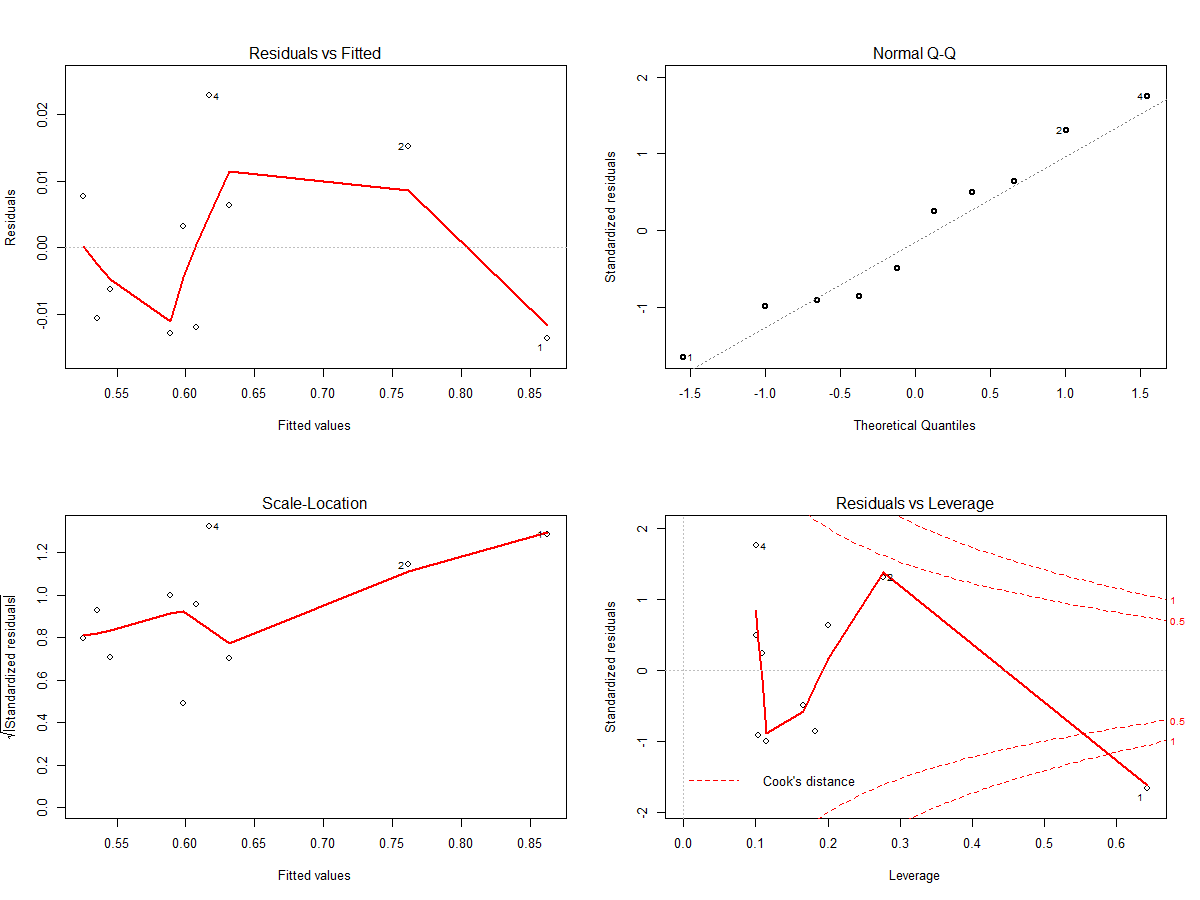
\includegraphics[width=16cm]{../fig/Tut10-08.png}
\begin{knitrout}
\definecolor{shadecolor}{rgb}{0.969, 0.969, 0.969}\color{fgcolor}
\includegraphics[width=\maxwidth]{figure/unnamed-chunk-45-1} 

\end{knitrout}
\end{center}
\caption{Serie de gráficos que se obtiene al usar {\tt plot(lmXY)} en R.}
\label{tut10:fig:GraficosDiagnosticoModeloLinealR}
\end{figure}


El primero de esos gráficos es precisamente una versión más elaborada del diagrama {\em residuos vs. predichos} que acabamos de aprender a construir. El siguiente es el {\em qq-plot} de los residuos estudentizados que también hemos comentado. El tercero es otra versión de {\em residuos vs. predichos}, que no vamos a discutir, y el cuarto tiene que ver con el contenido del próximo apartado. Así que volveremos allí sobre este gráfico.

\subsection{Residuos atípicos y puntos influyentes}

Vamos a empezar por el último de la serie de gráficos que se obtienen con {\tt plot(lmXY)} (ver Figura \ref{tut10:fig:GraficosDiagnosticoModeloLinealR}, pág. \pageref{tut10:fig:GraficosDiagnosticoModeloLinealR}). En este gráfico aparece representado el valor de la denominada {\sf distancia de Cook} para cada uno de los puntos de la muestra. La medida de Cook es una forma habitual de medir la {\em influencia} de un punto sobre el modelo de regresión, en el sentido que hemos discutido en la Sección  \ref{curso-cap10:subsec:ValoresAtipicosPuntosInfluyentesRegresion} del libro (página
\pageref{curso-cap10:subsec:ValoresAtipicosPuntosInfluyentesRegresion}).  No vamos a entrar en los detalles de cómo se define y calcula esa distancia, y nos limitaremos a decir que se suele utilizar, como referencia, el criterio de que un punto con un valor de la distancia de Cook mayor que uno es un {\em punto influyente}. En nuestro ejemplo, la figura muestra que uno de los puntos de la muestra es influyente. Además, para ayudarnos a localizarlo, R lo ha rotulado con la posición que ocupa dentro de la muestra, que es 1, la primera posición. El punto es $(0.25, 0.84892)$, que es el punto situado más a la izquierda en la Figura \ref{curso-cap10:fig:Anova02} del libro (pág. \pageref{curso-cap10:fig:Anova02}). ¿Puedes explicar, usando esa figura, la razón de que este punto sea influyente?

En cualquier caso, para ayudarte a visualizar en general lo que significa la {\em influencia} hemos preparado un fichero GeoGebra,
\begin{center}
\fichero{../ggb/Tut10-InterpretacionPuntoInfluyente.ggb}{Tut10-InterpretacionPuntoInfluyente.ggb}
\end{center}
con el que puedes explorar las ideas que ilustra la Figura c (pág. \pageref{curso-cap10:fig:ResiduosAtipicosPuntosInfluyentes}. Cuando abras ese fichero verás una imagen similar a esta:
\begin{center}
    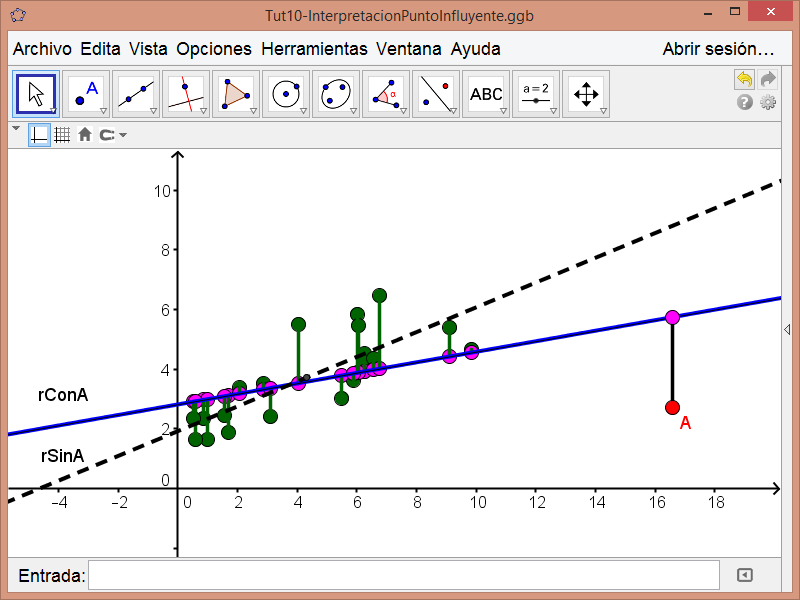
\includegraphics[width=15cm]{../fig/Tut10-23.png}
\end{center}
Como ves, se trata de un diagrama de dispersión con una nube de puntos (de color verde) y un punto adicional, el punto $A$ (de color rojo), que es el punto que podemos mover para experimentar con la idea de punto influyente. Además, se muestran las rectas de regresión correspondientes a la nube de puntos sin $A$ y también con $A$. La idea de influencia tiene que ver, precisamente, con la diferencia entre esas dos rectas. Para entenderlo lo mejor es que muevas el punto $A$ con el ratón, para ver como cambia la recta que lo tiene en cuenta. Puedes usar los distintos apartados de la Figura \pageref{curso-cap10:fig:ResiduosAtipicosPuntosInfluyentes} del libro como guía para cubrir todas las posibilidades que pueden darse.

En R disponemos de la función {\tt cooks.distance} para obtener esa distancia de Cook. Aplicada al Ejemplo \ref{curso-cap10:ejem:Anova01} de los puntos {\em ruidosos} del libro produce estos valores:
\begin{knitrout}
\definecolor{shadecolor}{rgb}{0.969, 0.969, 0.969}\color{fgcolor}\begin{kframe}
\begin{alltt}
\hlkwd{cooks.distance}\hlstd{(lmXY)}
\end{alltt}
\begin{verbatim}
##         1         2         3         4         5         6         7 
## 2.4844717 0.3266243 0.0133412 0.1722289 0.0486853 0.0035679 0.0645098 
##         8         9        10 
## 0.0250655 0.0826111 0.0504299
\end{verbatim}
\end{kframe}
\end{knitrout}
que confirman lo que vemos en la última gráfica de las cuatro que componen la Figura \ref{tut10:fig:GraficosDiagnosticoModeloLinealR}: el primer punto de la muestra es el único punto influyente de este ejemplo.

Fíjate en que, en este ejemplo, aunque ese punto es influyente su residuo no es atípico (puedes usar de nuevo la Figura \ref{curso-cap10:fig:Anova02} del libro como ayuda para ver esto).  De hecho, para comprobar si existe algún residuo atípico podemos utilizar la función {\tt outlierTest} de la librería {\tt car} de R.  Esta función realiza un tipo de contraste de hipótesis (basado en la $t$ de Student) para analizar la posible existencia de residuos atípicos. El resultado en este ejemplo es:
\begin{knitrout}
\definecolor{shadecolor}{rgb}{0.969, 0.969, 0.969}\color{fgcolor}\begin{kframe}
\begin{alltt}
\hlkwd{library}\hlstd{(car)}
\end{alltt}


{\ttfamily\noindent\color{warningcolor}{\#\# Warning: package 'car' was built under R version 3.3.2}}

{\ttfamily\noindent\itshape\color{messagecolor}{\#\# \\\#\# Attaching package: 'car'}}

{\ttfamily\noindent\itshape\color{messagecolor}{\#\# The following objects are masked from 'package:BSDA':\\\#\# \\\#\#\ \ \ \  Vocab, Wool}}

{\ttfamily\noindent\itshape\color{messagecolor}{\#\# The following object is masked from 'package:gtools':\\\#\# \\\#\#\ \ \ \  logit}}\begin{alltt}
\hlkwd{outlierTest}\hlstd{(lmXY)}
\end{alltt}
\begin{verbatim}
## 
## No Studentized residuals with Bonferonni p < 0.05
## Largest |rstudent|:
##   rstudent unadjusted p-value Bonferonni p
## 4   2.0856           0.075462      0.75462
\end{verbatim}
\end{kframe}
\end{knitrout}
En este caso, la frase {\tt No Studentized residuals with Bonferonni p < 0.05} nos informa de que no existen residuos atípicos. Si hubiera residuos atípicos, la función nos los devolvería como resultado. En este caso, al no existir residuos atípicos la función se limita a indicar cuál es el punto cuyo residuo tiene el mayor valor (absoluto), sin llegar a ser atípico.

\subsubsection*{La matriz $H$}

Volvamos a la medida de la influencia. En la Sección \ref{curso-cap10:subsec:ValoresAtipicosPuntosInfluyentesRegresion} del libro (pág. \pageref{curso-cap10:subsec:ValoresAtipicosPuntosInfluyentesRegresion}) hemos visto que la matriz $H$, la llamada {\em matriz sombrero}, permite medir fácilmente la influencia de cada punto de la muestra. En particular, nos interesan los valores de la diagonal de esta matriz, que en R se obtienen muy fácilmente así:
\begin{knitrout}
\definecolor{shadecolor}{rgb}{0.969, 0.969, 0.969}\color{fgcolor}\begin{kframe}
\begin{alltt}
\hlkwd{hatvalues}\hlstd{(lmXY)}
\end{alltt}
\begin{verbatim}
##       1       2       3       4       5       6       7       8       9 
## 0.64384 0.27704 0.10018 0.10100 0.10382 0.10846 0.11492 0.16650 0.18297 
##      10 
## 0.20126
\end{verbatim}
\end{kframe}
\end{knitrout}
Para usar estos valores como medida de la influencia utilizamos el  criterio de comparar los valores sombrero {(\em hatvalues)} con el valor $4/n$:
\begin{knitrout}
\definecolor{shadecolor}{rgb}{0.969, 0.969, 0.969}\color{fgcolor}\begin{kframe}
\begin{alltt}
\hlnum{4}\hlopt{/}\hlstd{n}
\end{alltt}
\begin{verbatim}
## [1] 0.4
\end{verbatim}
\begin{alltt}
\hlkwd{hatvalues}\hlstd{(lmXY)} \hlopt{>} \hlstd{(}\hlnum{4} \hlopt{/} \hlstd{n)}
\end{alltt}
\begin{verbatim}
##     1     2     3     4     5     6     7     8     9    10 
##  TRUE FALSE FALSE FALSE FALSE FALSE FALSE FALSE FALSE FALSE
\end{verbatim}
\end{kframe}
\end{knitrout}
Como puedes ver, el resultado confirma lo que ya habíamos establecido usando la distancia de Cook: el único punto influyente de esta muestra es el primer punto.


%En este caso,
%
%tiene que ver con su ``brazo de palanca''. En inglés, palanca (en este sentido) se dice {\em lever}, y por eso existe una medida de la influencia denominada {\sf leverage}. En español no hay, por lo que sé, una traducción universalmente aceptada para este término, aunque he visto utilizar ``efecto palanca'' para referirse a esto (y me parece adecuado).
%
%Para medir ese efecto palanca (leverage), se utiliza otro concepto relacionado, que son los (a falta de un nombre mejor) {\sf valores sombrero} (en inglés, {\sf hat values}). Estos valores, forman una matriz $n\cdot n$, la matriz sombrero $H$ ({\sf hat matrix}, en inglés), que se representa así:
%    \[H=\left(
%        \begin{array}{ccc}
%        h_{11}&\cdots&h_{1n}\\
%        &\ddots&\\
%        h_{n1}&\cdots&h_{nn}
%        \end{array}
%        \right)
%    \]
%y que tiene la propiedad de que:
%\[(\hat y_1,\ldots,\hat y_n) = (y_1,\ldots,y_n)\cdot H,\quad \mbox{(producto matricial).}\]
%Es decir, que para cualquier $i=1,\ldots,n$ es:
%\begin{equation}\label{cap10:ecu:valoresPalanca}
%    \hat y_j = h_{1j}\cdot y_1+h_{2j}\cdot y_2+\cdots+h_{nj}\cdot y_n.
%\end{equation}
%Esta relación muestra de donde proviene el nombre de la matriz $H$, y es porque transforma las $y_j$ en las $\hat y_j$ ($H$ le pone el sombrero a las $y_j$).
%
%¿Por qué son importantes estos valores sombrero $h_{ij}$ al tratar de medir la influencia? Imagínate que, manteniendo los mismos valores de $x_1,\ldots, x_n$, cambiásemos los valores $y_i$. Esta matriz nos diría cuáles serían los nuevos valores $\hat y_i$. Es decir, que esta matriz construye la recta de regresión. Además, la diagonal de esta matriz tiene una propiedad muy importante. Para cualquier elemento $h_{jj}$ de la diagonal se tiene:
%\begin{equation}\label{cap10:ecu:valoresPalanca2}
%    h_{ii}= h_{i1}^2+h_{i2}^2+\cdots+h_{in}^2.
%\end{equation}
%Y además, el valor $h_{ii}$ sólo depende de los $x_i$, como queda de manifiesto en esta relación:
%\[
%h_i=\dfrac{1}{n}+\dfrac{(x_i-\bar x)^2}{\displaystyle\sum_{j=1}^n(x_j-\bar x)^2}
%\]
%
%Los valores que aparecen elevados al cuadrado aquí (los de la fila $i$-ésima de $H$) son los que, de acuerdo con la Ecuación \ref{cap10:ecu:valoresPalanca}, determinan el peso que tiene el ingrediente $y_i$ a la hora de calcular cada uno de los $\hat y_j$. Es decir, que determinan el peso que tiene el valor $y_i$, asociado con el i-ésimo valor $x_i$ de la muestra. Puesto que además se cumple la Ecuación \ref{cap10:ecu:valoresPalanca2}, cada uno de los valores
%\[h_{11}, h_{12}, \ldots, h_{nn}\]
%puede utilizarse como un indicador de la influencia global sobre el modelo (sobre la recta) del valor $x_i$. Eso significa que podemos usar esos valores para medir el efecto palanca de los $x_i$.
%
%Afortunadamente, calcular estos valores con $R$ es muy fácil. Para obtenerlos en el ejemplo que estamos usando, basta con ejecutar (se muestra la salida)
%\begin{verbatim}
%> hatvalues(lmXY)
%        1         2         3         4         5
%0.6438400 0.2770361 0.1001842 0.1010030 0.1038231
%        6         7         8         9        10
%0.1084628 0.1149219 0.1665037 0.1829698 0.2012554
%\end{verbatim}
%Estos valores confirman que el efecto palanca (leverage), y por tanto la influencia, del primer punto es grande. Como regla práctica se utiliza el criterio de considerar como influyentes aquellos puntos $x_i$ cuya palanca (el valor $h_{ii}$ correspondiente) es mayor que dos veces el {\sf valor palanca medio}, que es sencillo ver que viene dado por:
%\[
%\bar h=\dfrac{2}{n}.
%\]
%En nuestro ejemplo, eso significa que $\bar h=\dfrac{2}{10}=0.2$. Así que un punto influyente, según este criterio, sería aquel cuyo efecto palanca sea mayor que $0.4$. Como se ve, en este ejemplo obtenemos el mismo resultado que cuando usábamos la distancia de Cook para medir la influencia. El segundo punto de la muestra tiene un valor mayor que la media, pero no llega a ser influyente.

\subsection{Bandas de confianza y predicción en R.}

En la Sección \ref{curso-cap10:subsec:BandasConfianzaPrediccion} del libro (pág. \pageref{curso-cap10:subsec:BandasConfianzaPrediccion}) hemos visto cómo se pueden definir las bandas de confianza y predicción para un modelo de regresión lineal simple que aparecen en la Figura \ref{curso-tut10:fig:BandasPrediccionConfianza} (pág. \pageref{curso-tut10:fig:BandasPrediccionConfianza}. Vamos a usar R para construir esas bandas, concretamente con la función {\tt predict} que ya hemos encontrado en la página \pageref{tut10:subsubsec:UsandoLmPredecirValores} de este tutorial.

Vamos a empezar por fabricar los datos del Ejemplo \ref{curso-cap10:ejem:Anova01} del libro (pág. \pageref{curso-cap10:ejem:Anova01}) y representarlos en un diagrama de dispersión, junto con la recta de regresión que obtenemos con {\tt lm}. También hemos añadido unos segmentos que ilustran los residuos de cada uno de los puntos de la muestra:
\begin{knitrout}
\definecolor{shadecolor}{rgb}{0.969, 0.969, 0.969}\color{fgcolor}\begin{kframe}
\begin{alltt}
\hlkwd{set.seed}\hlstd{(}\hlnum{2013}\hlstd{)}
\hlstd{n}\hlkwb{=}\hlnum{10}
\hlstd{x} \hlkwb{=} \hlkwd{sort}\hlstd{(}\hlkwd{signif}\hlstd{(}\hlkwd{runif}\hlstd{(n,} \hlkwc{min}\hlstd{=}\hlnum{0}\hlstd{,} \hlkwc{max}\hlstd{=}\hlnum{1} \hlstd{),} \hlkwc{digits}\hlstd{=}\hlnum{2}\hlstd{) )}
\hlstd{y} \hlkwb{=} \hlnum{1} \hlopt{-} \hlstd{(x}\hlopt{/}\hlnum{2}\hlstd{)} \hlopt{+} \hlkwd{rnorm}\hlstd{(n,}\hlkwc{sd}\hlstd{=}\hlnum{0.01}\hlstd{)}
\hlkwd{plot}\hlstd{(x, y,} \hlkwc{pch}\hlstd{=}\hlnum{4}\hlstd{,} \hlkwc{lwd}\hlstd{=}\hlnum{2}\hlstd{,} \hlkwc{col}\hlstd{=}\hlstr{"black"}\hlstd{,} \hlkwc{cex.lab}\hlstd{=}\hlnum{1.1}\hlstd{,} \hlkwc{cex.axis}\hlstd{=}\hlnum{1.1}\hlstd{)}
\hlkwd{box}\hlstd{(}\hlkwc{lwd}\hlstd{=}\hlnum{2}\hlstd{)}
\hlstd{lmXY} \hlkwb{=} \hlkwd{lm}\hlstd{(y} \hlopt{~} \hlstd{x)}
\hlkwd{abline}\hlstd{(lmXY,} \hlkwc{lwd}\hlstd{=}\hlnum{2}\hlstd{,} \hlkwc{col}\hlstd{=}\hlstr{"blue"}\hlstd{)}
\hlkwd{segments}\hlstd{(x,}\hlkwd{fitted}\hlstd{(lmXY), x, y,} \hlkwc{lwd}\hlstd{=}\hlnum{2}\hlstd{)}
\end{alltt}
\end{kframe}
\includegraphics[width=\maxwidth]{figure/tut10_bandasConfianza01-1} 

\end{knitrout}
A continuación vamos a crear una sucesión de puntos que cubran todo el recorrido de valores de $x$ en la muestra. Usaremos un total de $50$ puntos, pero puedes usar más para conseguir mayor nivel de detalle.
\begin{knitrout}
\definecolor{shadecolor}{rgb}{0.969, 0.969, 0.969}\color{fgcolor}\begin{kframe}
\begin{alltt}
\hlstd{pred.x} \hlkwb{=} \hlkwd{seq}\hlstd{(}\hlkwd{min}\hlstd{(x),} \hlkwd{max}\hlstd{(x),} \hlkwc{length.out}\hlstd{=}\hlnum{50}\hlstd{)}
\end{alltt}
\end{kframe}
\end{knitrout}
Ahora viene el paso clave. Usamos {\tt predict} para crear los intervalos de confianza y predicción para cada uno de los puntos de {\tt pred.x}. La opción {\tt int} de {\tt predict} nos permite seleccionar el tipo de intervalo que se crea en cada caso. Usaremos un nivel de confianza del 95\%. El resultado son dos data.frames de los que mostramos las primeras líneas:

\begin{knitrout}
\definecolor{shadecolor}{rgb}{0.969, 0.969, 0.969}\color{fgcolor}\begin{kframe}
\begin{alltt}
\hlstd{predct.intrvl} \hlkwb{=} \hlkwd{predict}\hlstd{(lmXY,} \hlkwc{int}\hlstd{=}\hlstr{"p"}\hlstd{,} \hlkwc{newdata}\hlstd{=}\hlkwd{data.frame}\hlstd{(}\hlkwc{x} \hlstd{= pred.x),} \hlkwc{level}\hlstd{=}\hlnum{0.95}\hlstd{)}
\hlstd{confd.intrvl} \hlkwb{=} \hlkwd{predict}\hlstd{(lmXY,} \hlkwc{int}\hlstd{=}\hlstr{"c"}\hlstd{,} \hlkwc{newdata}\hlstd{=}\hlkwd{data.frame}\hlstd{(}\hlkwc{x} \hlstd{= pred.x),} \hlkwc{level}\hlstd{=}\hlnum{0.95}\hlstd{)}
\hlkwd{head}\hlstd{(predct.intrvl)}
\end{alltt}
\begin{verbatim}
##       fit     lwr     upr
## 1 0.86255 0.82183 0.90328
## 2 0.85568 0.81535 0.89602
## 3 0.84882 0.80886 0.88877
## 4 0.84195 0.80237 0.88153
## 5 0.83508 0.79586 0.87429
## 6 0.82821 0.78935 0.86707
\end{verbatim}
\begin{alltt}
\hlkwd{head}\hlstd{(confd.intrvl)}
\end{alltt}
\begin{verbatim}
##       fit     lwr     upr
## 1 0.86255 0.83707 0.88804
## 2 0.85568 0.83082 0.88054
## 3 0.84882 0.82458 0.87305
## 4 0.84195 0.81833 0.86556
## 5 0.83508 0.81208 0.85807
## 6 0.82821 0.80583 0.85059
\end{verbatim}
\end{kframe}
\end{knitrout}
Como ves, en ambos casos se obtiene un {\tt data.frame} con tres columnas que contienen, respectivamente el centro y los extremos inferior y superior del intervalo correspondiente, ya sea de predicción o de confianza.

El trabajo duro ya está hecho, ahora sólo hay que representar gráficamente esas bandas de predicción y confianza. Para eso lo más cómodo es usar la función {\tt matlines} que nos va a permitir dibujar en un mismo gráfico simultáneamente los valores de varias columnas de una matriz. Para que lo entiendas en un ejemplo sencillo, vamos a usar {\tt matlines} para dibujar en un mismo gráfico las curvas $y = \sen(x)$, $y = \cos(x)$ e $y=\sen(3x)$. Lo haremos creando primero una sucesión de $200$ puntos $x$ distribuidos uniformemente de $0$ a $2\pi$:
\begin{knitrout}
\definecolor{shadecolor}{rgb}{0.969, 0.969, 0.969}\color{fgcolor}\begin{kframe}
\begin{alltt}
\hlstd{x} \hlkwb{=} \hlkwd{seq}\hlstd{(}\hlnum{0}\hlstd{,} \hlnum{2} \hlopt{*} \hlstd{pi,} \hlkwc{length.out}\hlstd{=}\hlnum{200}\hlstd{)}
\end{alltt}
\end{kframe}
\end{knitrout}
Y ahora hacemos el gráfico con {\tt matlines}. Primero dibujamos una de las curvas con {\tt plot} y la opción {\verb#type="n"#}. Este comando crea una ventana gráfica de las dimensiones adecuadas, pero no dibuja nada en ella (por el {\verb#tyype="n"#}), en la que luego {\tt matlines} se encargará de añadir las gráficas. Hemos elegido además los colores y tipo de trazo de las curvas:
{\small
\begin{knitrout}
\definecolor{shadecolor}{rgb}{0.969, 0.969, 0.969}\color{fgcolor}\begin{kframe}
\begin{alltt}
\hlkwd{plot}\hlstd{(x,} \hlkwd{sin}\hlstd{(x),} \hlkwc{type}\hlstd{=}\hlstr{"n"}\hlstd{)}
\hlkwd{matlines}\hlstd{(x,} \hlkwd{cbind}\hlstd{(}\hlkwd{sin}\hlstd{(x),} \hlkwd{cos}\hlstd{(x),} \hlkwd{sin}\hlstd{(}\hlnum{2}\hlopt{*}\hlstd{x),} \hlkwc{lwd}\hlstd{=}\hlnum{3}\hlstd{),}
    \hlkwc{col}\hlstd{=}\hlkwd{c}\hlstd{(}\hlstr{"red"}\hlstd{,} \hlstr{"blue"}\hlstd{,} \hlstr{"black"}\hlstd{),} \hlkwc{lty}\hlstd{=}\hlnum{1}\hlstd{)}
\end{alltt}
\end{kframe}
\includegraphics[width=\maxwidth]{figure/unnamed-chunk-53-1} 

\end{knitrout}
}
Volviendo al dibujo de las bandas de confianza y predicción, el límite superior de la banda de predicción es una curva que recorre los extremos superiores de los intervalos de predicción para cada punto del recorrido de la variable $x$ en los puntos de la muestra. Y análogamente para el resto de curvas que definen las bandas de predicción y confianza. Podemos, por tanto, usar {\tt matlines} para añadir esas bandas al gráfico de dispersión anterior, usando las columnas $2$ y $3$ de los {\tt data.frames} que hemos construido para almacenar esas bandas. La única diferencia con el gráfico original está en las dos últimas instrucciones:
\begin{knitrout}
\definecolor{shadecolor}{rgb}{0.969, 0.969, 0.969}\color{fgcolor}\begin{kframe}
\begin{alltt}
\hlkwd{set.seed}\hlstd{(}\hlnum{2013}\hlstd{)}
\hlstd{n}\hlkwb{=}\hlnum{10}
\hlstd{x} \hlkwb{=} \hlkwd{sort}\hlstd{(}\hlkwd{signif}\hlstd{(}\hlkwd{runif}\hlstd{(n,} \hlkwc{min}\hlstd{=}\hlnum{0}\hlstd{,} \hlkwc{max}\hlstd{=}\hlnum{1} \hlstd{),} \hlkwc{digits}\hlstd{=}\hlnum{2}\hlstd{) )}
\hlstd{y} \hlkwb{=} \hlnum{1} \hlopt{-} \hlstd{(x}\hlopt{/}\hlnum{2}\hlstd{)} \hlopt{+} \hlkwd{rnorm}\hlstd{(n,}\hlkwc{sd}\hlstd{=}\hlnum{0.01}\hlstd{)}
\hlkwd{plot}\hlstd{(x, y,} \hlkwc{pch}\hlstd{=}\hlnum{4}\hlstd{,} \hlkwc{lwd}\hlstd{=}\hlnum{2}\hlstd{,} \hlkwc{col}\hlstd{=}\hlstr{"black"}\hlstd{,} \hlkwc{cex.lab}\hlstd{=}\hlnum{1.1}\hlstd{,} \hlkwc{cex.axis}\hlstd{=}\hlnum{1.1}\hlstd{)}
\hlkwd{box}\hlstd{(}\hlkwc{lwd}\hlstd{=}\hlnum{2}\hlstd{)}
\hlstd{lmXY} \hlkwb{=} \hlkwd{lm}\hlstd{(y} \hlopt{~} \hlstd{x)}
\hlkwd{abline}\hlstd{(lmXY,} \hlkwc{lwd}\hlstd{=}\hlnum{2}\hlstd{,} \hlkwc{col}\hlstd{=}\hlstr{"blue"}\hlstd{)}
\hlkwd{segments}\hlstd{(x,}\hlkwd{fitted}\hlstd{(lmXY), x, y,} \hlkwc{lwd}\hlstd{=}\hlnum{2}\hlstd{)}
\hlkwd{matlines}\hlstd{(pred.x, predct.intrvl[ ,}\hlnum{2}\hlopt{:}\hlnum{3}\hlstd{],} \hlkwc{lty}\hlstd{=}\hlkwd{c}\hlstd{(}\hlnum{1}\hlstd{,} \hlnum{1}\hlstd{,} \hlnum{1}\hlstd{),} \hlkwc{col}\hlstd{=}\hlstr{"red"}\hlstd{,} \hlkwc{lwd}\hlstd{=}\hlnum{2}\hlstd{)}
\hlkwd{matlines}\hlstd{(pred.x, confd.intrvl[ ,}\hlnum{2}\hlopt{:}\hlnum{3}\hlstd{],} \hlkwc{lty}\hlstd{=}\hlkwd{c}\hlstd{(}\hlnum{1}\hlstd{,} \hlnum{1}\hlstd{,} \hlnum{1}\hlstd{),} \hlkwc{col}\hlstd{=}\hlstr{"darkgreen"}\hlstd{,} \hlkwc{lwd}\hlstd{=}\hlnum{2}\hlstd{)}
\end{alltt}
\end{kframe}
\includegraphics[width=\maxwidth]{figure/tut10_bandasConfianza02-1} 

\end{knitrout}
A diferencia de lo que hemos hecho en el libro, aquí hemos usado curvas de trazo continuo para el límite de las gráficas. Puedes cambiar los valores de {\tt lty} para experimentar otras posibilidades.


\subsection{El cuarteto de Anscombe en R.}

%Ninguna discusión del modelo de regresión lineal simple estaría completa sin incluir esta colección de ejemplos, ya clásicos, debidos al estadístico inglés Frank Anscombe.
%\begin{center}
%\link{http://en.wikipedia.org/wiki/Francis_Anscombe}{http://en.wikipedia.org/wiki/Francis\_Anscombe}
%\end{center}
%Se trata de cuatro muestras,  cada una de ellas formada por $11$ puntos $(x_i,y_i)$, que tienen muchas propiedades estadísticas prácticamente iguales. Por ejemplo, las cuatro muestras tienen los mismos valores de
%\begin{itemize}
%  \item $\bar x=9$
%  \item $\bar y\approx 7.50$
%  \item $s^2_x=11$
%  \item $s^2_y\approx 4.1$
%  \item $\Cov(x,y)\approx 5.5$
%  \item $r\approx 0.816$
%\end{itemize}
%y en particular, en los cuatro casos la recta de regresión es aproximadamente (con tres cifras significativas):
%\[y = 3+5\cdot x.\]
%Sin embargo, los diagramas de dispersión de los cuatro casos, que aparecen en la Figura \ref{tut10:fig:CuartetoAnscombe} muestran que las cuatro situaciones son claramente distintas.
%\begin{figure}[b!]
%\begin{center}
%    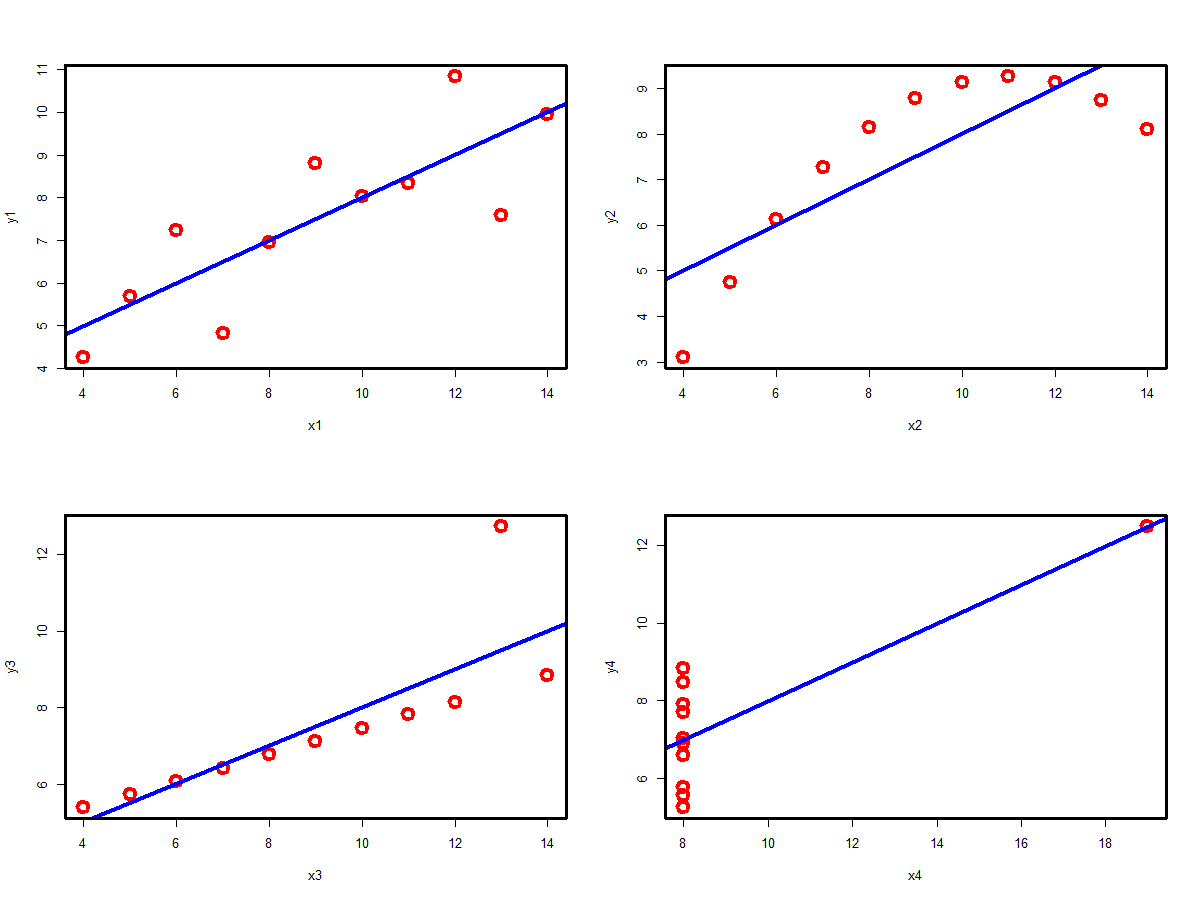
\includegraphics[width=15cm]{../fig/Tut10-Anscombe.png}
%\end{center}
%\caption{Diagramas de dispersión de los cuatro casos del {\em Cuarteto de Anscombe}.}
%\label{tut10:fig:CuartetoAnscombe}
%\end{figure}
%
%\begin{itemize}
%  \item En el primer caso, la recta de regresión es un  buen modelo del conjunto de puntos.
%  \item En el segundo caso, la relación entre las variables $X$ e $Y$ es, obviamente, no lineal, y lo que se necesita es un ajuste polinómico. Volveremos sobre este caso en el apartado \ref{tut10:RegresionPolinomicaR} de este tutorial.
%  \item El tercer caso contiene un punto (concretamente el $(x_3,y_3)$) con un residuo atípico, que además es influyente (su {\em efecto palanca} no es grande, pero su distancia de Cook es mayor que uno).
%  \item El cuarto caso es, en algún sentido, el más patológico. Todos los valores $x_i$ son iguales excepto uno ($x_8$ para ser precisos). Así que si se elimina el punto $(x_8,y_8)$, los restantes puntos están en una recta vertical (y el modelo de regresión que hemos visto en el Capítulo \ref{curso-cap:RegresionLinealSimple} no sirve, porque no es capaz de producir rectas verticales). Es interesante observar que el punto $(x_8,y_8)$ es, obviamente, influyente, pero que su residuo no es atípico.
%\end{itemize}

En R, como parte de la instalación básica, disponemos de un {\tt dataframe} llamado {\tt anscombe}, con variables {\tt x1, x2, x3, x4, y1, y2, y3, y4}, y que contiene los valores de estos ejemplos. Para verlos basta con que hagas:
\begin{knitrout}
\definecolor{shadecolor}{rgb}{0.969, 0.969, 0.969}\color{fgcolor}\begin{kframe}
\begin{alltt}
\hlstd{anscombe}
\end{alltt}
\begin{verbatim}
##    x1 x2 x3 x4    y1   y2    y3    y4
## 1  10 10 10  8  8.04 9.14  7.46  6.58
## 2   8  8  8  8  6.95 8.14  6.77  5.76
## 3  13 13 13  8  7.58 8.74 12.74  7.71
## 4   9  9  9  8  8.81 8.77  7.11  8.84
## 5  11 11 11  8  8.33 9.26  7.81  8.47
## 6  14 14 14  8  9.96 8.10  8.84  7.04
## 7   6  6  6  8  7.24 6.13  6.08  5.25
## 8   4  4  4 19  4.26 3.10  5.39 12.50
## 9  12 12 12  8 10.84 9.13  8.15  5.56
## 10  7  7  7  8  4.82 7.26  6.42  7.91
## 11  5  5  5  8  5.68 4.74  5.73  6.89
\end{verbatim}
\end{kframe}
\end{knitrout}
Vamos a comprobar lo que hemos dicho sobre los valores comunes a las cuatro muestras. Usaremos {\tt apply} para calcular la media y cuasivarianza por columnas del {\tt data.frame}:
\begin{knitrout}
\definecolor{shadecolor}{rgb}{0.969, 0.969, 0.969}\color{fgcolor}\begin{kframe}
\begin{alltt}
\hlkwd{apply}\hlstd{(anscombe,} \hlnum{2}\hlstd{, mean)}
\end{alltt}
\begin{verbatim}
##     x1     x2     x3     x4     y1     y2     y3     y4 
## 9.0000 9.0000 9.0000 9.0000 7.5009 7.5009 7.5000 7.5009
\end{verbatim}
\begin{alltt}
\hlkwd{apply}\hlstd{(anscombe,} \hlnum{2}\hlstd{, var)}
\end{alltt}
\begin{verbatim}
##      x1      x2      x3      x4      y1      y2      y3      y4 
## 11.0000 11.0000 11.0000 11.0000  4.1273  4.1276  4.1226  4.1232
\end{verbatim}
\end{kframe}
\end{knitrout}
Para calcular la covarianza de cada una de las muestras hacemos un pequeño truco con {\tt sapply} y una función anónima. Es un poco más avanzado que otras cosas que hemos hecho con R, pero si no lo entiendes siempre puedes hacer las cuentas más a mano:
\begin{knitrout}
\definecolor{shadecolor}{rgb}{0.969, 0.969, 0.969}\color{fgcolor}\begin{kframe}
\begin{alltt}
\hlkwd{sapply}\hlstd{(}\hlnum{1}\hlopt{:}\hlnum{4}\hlstd{,} \hlkwa{function}\hlstd{(}\hlkwc{x}\hlstd{)\{}\hlkwd{cov}\hlstd{(anscombe[ ,x], anscombe[ , x} \hlopt{+} \hlnum{4}\hlstd{])\})}
\end{alltt}
\begin{verbatim}
## [1] 5.501 5.500 5.497 5.499
\end{verbatim}
\end{kframe}
\end{knitrout}
Y para el coeficiente de correlación un truco análogo:
\begin{knitrout}
\definecolor{shadecolor}{rgb}{0.969, 0.969, 0.969}\color{fgcolor}\begin{kframe}
\begin{alltt}
\hlkwd{sapply}\hlstd{(}\hlnum{1}\hlopt{:}\hlnum{4}\hlstd{,} \hlkwa{function}\hlstd{(}\hlkwc{x}\hlstd{)\{}\hlkwd{cor}\hlstd{(anscombe[ ,x], anscombe[ , x} \hlopt{+} \hlnum{4}\hlstd{])\})}
\end{alltt}
\begin{verbatim}
## [1] 0.81642 0.81624 0.81629 0.81652
\end{verbatim}
\end{kframe}
\end{knitrout}
Para dibujar de forma sencilla uno de estos ejemplos puedes hacer:
\begin{knitrout}
\definecolor{shadecolor}{rgb}{0.969, 0.969, 0.969}\color{fgcolor}\begin{kframe}
\begin{alltt}
\hlstd{(lmA1}\hlkwb{=}\hlkwd{lm}\hlstd{(anscombe[,} \hlnum{5}\hlstd{]} \hlopt{~} \hlstd{anscombe[ ,} \hlnum{1}\hlstd{]))}
\end{alltt}
\begin{verbatim}
## 
## Call:
## lm(formula = anscombe[, 5] ~ anscombe[, 1])
## 
## Coefficients:
##   (Intercept)  anscombe[, 1]  
##           3.0            0.5
\end{verbatim}
\begin{alltt}
\hlkwd{plot}\hlstd{(anscombe[ ,} \hlnum{1}\hlstd{], anscombe[ ,} \hlnum{5}\hlstd{],} \hlkwc{col}\hlstd{=}\hlstr{"red"}\hlstd{,} \hlkwc{lwd}\hlstd{=}\hlnum{4}\hlstd{,} \hlkwc{cex}\hlstd{=}\hlnum{2}\hlstd{)}
\hlkwd{abline}\hlstd{(lmA1,} \hlkwc{col}\hlstd{=}\hlstr{"blue"}\hlstd{,} \hlkwc{lwd}\hlstd{=}\hlnum{4}\hlstd{)}
\hlkwd{box}\hlstd{(}\hlkwc{lwd}\hlstd{=}\hlnum{3}\hlstd{,}\hlkwc{bty}\hlstd{=}\hlstr{"o"}\hlstd{)}
\end{alltt}
\end{kframe}

{\centering \includegraphics[width=\maxwidth]{figure/unnamed-chunk-58-1} 

}



\end{knitrout}
Si lo que queremos es un diagnóstico sencillo de este modelo de regresión podemos hacer:
\begin{knitrout}
\definecolor{shadecolor}{rgb}{0.969, 0.969, 0.969}\color{fgcolor}\begin{kframe}
\begin{alltt}
\hlkwd{studres}\hlstd{(lmA1)}
\end{alltt}
\begin{verbatim}
##         1         2         3         4         5         6         7 
##  0.031345 -0.040845 -2.081099  1.126800 -0.139801 -0.038196  1.116959 
##         8         9        10        11 
## -0.704581  1.838330 -1.568460  0.156809
\end{verbatim}
\begin{alltt}
\hlkwd{outlierTest}\hlstd{(lmA1)}
\end{alltt}
\begin{verbatim}
## 
## No Studentized residuals with Bonferonni p < 0.05
## Largest |rstudent|:
##   rstudent unadjusted p-value Bonferonni p
## 3  -2.0811           0.070994      0.78093
\end{verbatim}
\begin{alltt}
\hlkwd{hatvalues}\hlstd{(lmA1)}
\end{alltt}
\begin{verbatim}
##        1        2        3        4        5        6        7        8 
## 0.100000 0.100000 0.236364 0.090909 0.127273 0.318182 0.172727 0.318182 
##        9       10       11 
## 0.172727 0.127273 0.236364
\end{verbatim}
\begin{alltt}
\hlkwd{hatvalues}\hlstd{(lmA1)} \hlopt{>} \hlnum{2} \hlopt{*} \hlkwd{mean}\hlstd{(}\hlkwd{hatvalues}\hlstd{(lmA1))}
\end{alltt}
\begin{verbatim}
##     1     2     3     4     5     6     7     8     9    10    11 
## FALSE FALSE FALSE FALSE FALSE FALSE FALSE FALSE FALSE FALSE FALSE
\end{verbatim}
\begin{alltt}
\hlkwd{cooks.distance}\hlstd{(lmA1)}
\end{alltt}
\begin{verbatim}
##           1           2           3           4           5           6 
## 0.000061398 0.000104247 0.489209276 0.061636999 0.001599342 0.000382900 
##           7           8           9          10          11 
## 0.126756485 0.122699896 0.279029593 0.154341222 0.004268011
\end{verbatim}
\begin{alltt}
\hlkwd{gvlma}\hlstd{(lmA1)}
\end{alltt}


{\ttfamily\noindent\bfseries\color{errorcolor}{\#\# Error in eval(expr, envir, enclos): no se pudo encontrar la funci'on "{}gvlma"{}}}\end{kframe}
\end{knitrout}
Te proponemos unos ejercicios adicionales para completar el estudio del {\em cuarteto de Anscombe}:
\begin{ejercicio}
\label{tut10:ejercicio08}
\begin{enumerate}
  \item[]
  \item Interpreta los resultados anteriores en términos de la validez del modelo, presencia de puntos influyentes, etc.
  \item Usa la función {\tt plot} para hacer un diagnóstico gráfico de este modelo de regresión.

  \item Haz un diagnóstico de los modelos de regresión lineal simples correspondientes a los otros tres integrantes del {\em cuarteto}.
\end{enumerate}
\qed
\end{ejercicio}

La advertencia fundamental que hay que extraer de estos cuatro ejemplos es que el coeficiente de correlación $r$, no puede servir por si mismo como indicador de la calidad de un modelo de regresión lineal. Pero, abundando en esa dirección, también hay que observar que ningún análisis de regresión puede considerarse completo si no se incluye la exploración de los datos (y lo mismo sirve para cualquier análisis estadístico). La exploración gráfica, pero también un análisis minucioso de las condiciones del modelo, son herramientas imprescindibles, sin las cuales corremos el riesgo de que nuestras conclusiones carezcan de fundamento.



\section{Modelos de regresión, más allá de las rectas.}
\noindent{\bf Opcional: esta sección puede omitirse en una primera lectura. }

La Sección \ref{curso-cap10:sec:ModelosDeRegresion} del libro (pág. \pageref{curso-cap10:sec:ModelosDeRegresion}) comienza con el Ejemplo \ref{curso-cap10:ejem:RegresionNoLineal}, en el que mediante un cambio de variable reducimos la construcción de un modelo de la forma
\[  y=a_0\cdot x^{a_1}\]
a la de un modelo
\[\tilde y=b_0+b_1\cdot\tilde x.\]
donde
\[
\begin{cases}
\tilde x=\ln x,\\
\tilde y=\ln y,\\
b_0=\ln a_0,\\
b_1=a_1,
\end{cases}
\]
Los puntos de ese ejemplo se han construido en R con este código
\begin{knitrout}
\definecolor{shadecolor}{rgb}{0.969, 0.969, 0.969}\color{fgcolor}\begin{kframe}
\begin{alltt}
\hlkwd{set.seed}\hlstd{(}\hlnum{2014}\hlstd{)}
\hlstd{n}\hlkwb{=}\hlnum{20}
\hlstd{x}\hlkwb{=}\hlkwd{sort}\hlstd{(}\hlkwd{signif}\hlstd{(}\hlkwd{runif}\hlstd{(n,}\hlkwc{min}\hlstd{=}\hlnum{10}\hlstd{,}\hlkwc{max}\hlstd{=}\hlnum{25}\hlstd{),}\hlkwc{digits}\hlstd{=}\hlnum{3}\hlstd{))}
\hlstd{y}\hlkwb{=}\hlkwd{round}\hlstd{(}\hlnum{3e-4} \hlopt{*} \hlstd{x}\hlopt{^}\hlstd{(}\hlnum{26}\hlopt{/}\hlnum{7}\hlstd{)} \hlopt{*} \hlkwd{exp}\hlstd{(}\hlkwd{rnorm}\hlstd{(n,} \hlnum{0}\hlstd{,} \hlnum{0.1}\hlstd{)),}\hlkwc{digits}\hlstd{=}\hlnum{1}\hlstd{)}
\end{alltt}
\end{kframe}
\end{knitrout}
¿Puedes ver por qué ese código produce una colección de puntos adecuada para el modelo que nos planteamos en este ejemplo? Fíjate en particular en el término de error {\tt exp(rnorm(n, 0, 0.1)} que nos garantiza que una vez aplicado el cambio de variable podremos aplicar con éxito un modelo lineal simple.

\begin{ejercicio}
\label{tut10:ejercicio09}
\begin{enumerate}
  \item[]
  \item Usa R para construir los puntos $(\tilde x, \tilde y)$ de este ejemplo. Recuerda que el logaritmo neperiano se obtiene en R con  {\tt log}.
  \item Construye (usando una plantilla o la función {\tt lm}) el modelo lineal para esa muestra de puntos $(\tilde x, \tilde y)$, y comprueba los resultados del Ejemplo \ref{curso-cap10:ejem:RegresionNoLineal} del libro.
  \item Adicionalmente, puedes tratar de reproducir la Figura \ref{curso-cap10:fig:EjemploRegresionNoLineal02} del libro (pág. \pageref{cap10:fig:EjemploRegresionNoLineal02}) usando la función {\tt curve} para dibujar la función exponencial.
\end{enumerate}
\qed
\end{ejercicio}


\subsection*{Regresión polinómica en R.}
\label{tut10:subsec:regresionPolinomicaR}

Vamos a aprovechar el segundo miembro del cuarteto de Anscombe para introducirnos en el terreno de la regresión polinómica con R. Ese ejemplo en particular (que aparece en la parte superior derecha de la Figura \ref{curso-tut10:fig:CuartetoAnscombe} del libro, pág. \pageref{curso-tut10:fig:CuartetoAnscombe}) requiere el uso de una parábola en lugar de una recta. La ecuación de esa parábola será de la forma:
\[y=b_0+b_1\cdot x+b_2\cdot x^2\]
para ciertos coeficientes $b_0, b_1, b_2$.

¿Cómo podemos usar R para averiguar cuál es la mejor parábola posible? Es decir, para localizar los valores adecuados de $b_0, b_1, b_2$. Pues usando, de nuevo, la función {\tt lm}, pero con una sintaxis ligeramente más complicada. Para ilustrarlo, empezamos por crear dos vectores con las coordenadas $x$ e $y$ de este ejemplo:
\begin{knitrout}
\definecolor{shadecolor}{rgb}{0.969, 0.969, 0.969}\color{fgcolor}\begin{kframe}
\begin{alltt}
 \hlstd{(x} \hlkwb{=} \hlstd{anscombe}\hlopt{$}\hlstd{x2)}
\end{alltt}
\begin{verbatim}
##  [1] 10  8 13  9 11 14  6  4 12  7  5
\end{verbatim}
\begin{alltt}
 \hlstd{(y} \hlkwb{=} \hlstd{anscombe}\hlopt{$}\hlstd{y2)}
\end{alltt}
\begin{verbatim}
##  [1] 9.14 8.14 8.74 8.77 9.26 8.10 6.13 3.10 9.13 7.26 4.74
\end{verbatim}
\end{kframe}
\end{knitrout}
Y ahora, para crear ese modelo polinómico de grado dos basta con usar este código:
\begin{knitrout}
\definecolor{shadecolor}{rgb}{0.969, 0.969, 0.969}\color{fgcolor}\begin{kframe}
\begin{alltt}
\hlstd{(lmPolXY}\hlkwb{=}\hlkwd{lm}\hlstd{(y} \hlopt{~} \hlkwd{I}\hlstd{(x)} \hlopt{+} \hlkwd{I}\hlstd{(x}\hlopt{^}\hlnum{2}\hlstd{)))}
\end{alltt}
\begin{verbatim}
## 
## Call:
## lm(formula = y ~ I(x) + I(x^2))
## 
## Coefficients:
## (Intercept)         I(x)       I(x^2)  
##      -5.996        2.781       -0.127
\end{verbatim}
\end{kframe}
\end{knitrout}
La peculiar notación \verb# I(x) + I(x^2)# se debe a que, por defecto, si escribiéramos simplemente:
\begin{knitrout}
\definecolor{shadecolor}{rgb}{0.969, 0.969, 0.969}\color{fgcolor}\begin{kframe}
\begin{alltt}
\hlkwd{lm}\hlstd{(y} \hlopt{~} \hlstd{x} \hlopt{+} \hlstd{x}\hlopt{^}\hlnum{2}\hlstd{)}
\end{alltt}
\begin{verbatim}
## 
## Call:
## lm(formula = y ~ x + x^2)
## 
## Coefficients:
## (Intercept)            x  
##         3.0          0.5
\end{verbatim}
\end{kframe}
\end{knitrout}
R usaría los denominados {\sf polinomios ortogonales}, un tipo especial de polinomios que tienen propiedades que los hacen muy útiles en este contexto. Como de costumbre, R tiende a proporcionar la mejor solución, pero esa, a menudo, no es la que queremos ver cuando estamos aprendiendo a hacer las cosas por primera vez. El precio que pagaremos, en este caso, es esa notación un poco más complicada con la {\tt I}.

Usando esa notación, en cualquier caso, obtenemos el modelo parabólico que andábamos buscando. En particular, los coeficientes $b_0$, $b_1$ y $b_2$ quedan almacenados en un vector, al que podemos acceder usando la componente {\tt coefficients} del resultado de la función {\tt lm}. Para este ejemplo, y usando {\tt b} como nombre del vector para mantener la notación que nos es familiar, hacemos:
\begin{knitrout}
\definecolor{shadecolor}{rgb}{0.969, 0.969, 0.969}\color{fgcolor}\begin{kframe}
\begin{alltt}
\hlstd{(b} \hlkwb{=} \hlstd{lmPolXY}\hlopt{$}\hlstd{coefficients)}
\end{alltt}
\begin{verbatim}
## (Intercept)        I(x)      I(x^2) 
##    -5.99573     2.78084    -0.12671
\end{verbatim}
\end{kframe}
\end{knitrout}
Pero cuidado al usar este vector, porque hay un desplazamiento en los índices: {\tt b[1], b[2]} y {\tt b[3]} corresponden a $b_0$, $b_1$ y $b_2$ respectivamente.

En la Figura \ref{tut10:fig:RegresionPolinomica} (pág. \pageref{tut10:fig:RegresionPolinomica}) se muestra la parábola que hemos obtenido, que en este caso pasa exactamente por los puntos del segundo ejemplo de Anscombe. Se muestra además la recta de regresión que obtenemos con \verb#lm(y~x)#. Como puedes ver, el modelo que proporciona la recta  no es adecuado. El código R que hemos usado para producir esa figura es este:
\begin{knitrout}
\definecolor{shadecolor}{rgb}{0.969, 0.969, 0.969}\color{fgcolor}\begin{kframe}
\begin{alltt}
\hlkwd{plot}\hlstd{(anscombe[ ,} \hlnum{2}\hlstd{], anscombe[ ,} \hlnum{6}\hlstd{],} \hlkwc{col}\hlstd{=}\hlstr{"red"}\hlstd{,} \hlkwc{lwd}\hlstd{=}\hlnum{2}\hlstd{,} \hlkwc{cex}\hlstd{=}\hlnum{1.1}\hlstd{)}
\hlkwd{curve}\hlstd{(b[}\hlnum{1}\hlstd{]} \hlopt{+} \hlstd{b[}\hlnum{2}\hlstd{]} \hlopt{*} \hlstd{x} \hlopt{+} \hlstd{b[}\hlnum{3}\hlstd{]} \hlopt{*} \hlstd{x}\hlopt{^}\hlnum{2}\hlstd{,}
    \hlkwc{add} \hlstd{=} \hlnum{TRUE}\hlstd{,} \hlkwc{from} \hlstd{=} \hlnum{3}\hlstd{,} \hlkwc{to} \hlstd{=} \hlnum{15}\hlstd{,} \hlkwc{col}\hlstd{=}\hlstr{"blue"}\hlstd{,} \hlkwc{lwd}\hlstd{=}\hlnum{2}\hlstd{)}
\hlkwd{abline}\hlstd{(}\hlkwd{lm}\hlstd{(anscombe[ ,} \hlnum{6}\hlstd{]} \hlopt{~} \hlstd{anscombe[ ,} \hlnum{2}\hlstd{]),} \hlkwc{lwd}\hlstd{=}\hlnum{2}\hlstd{,} \hlkwc{lty}\hlstd{=}\hlnum{2}\hlstd{)}
\end{alltt}
\end{kframe}
\end{knitrout}

\begin{figure}[b!]
\begin{center}
    %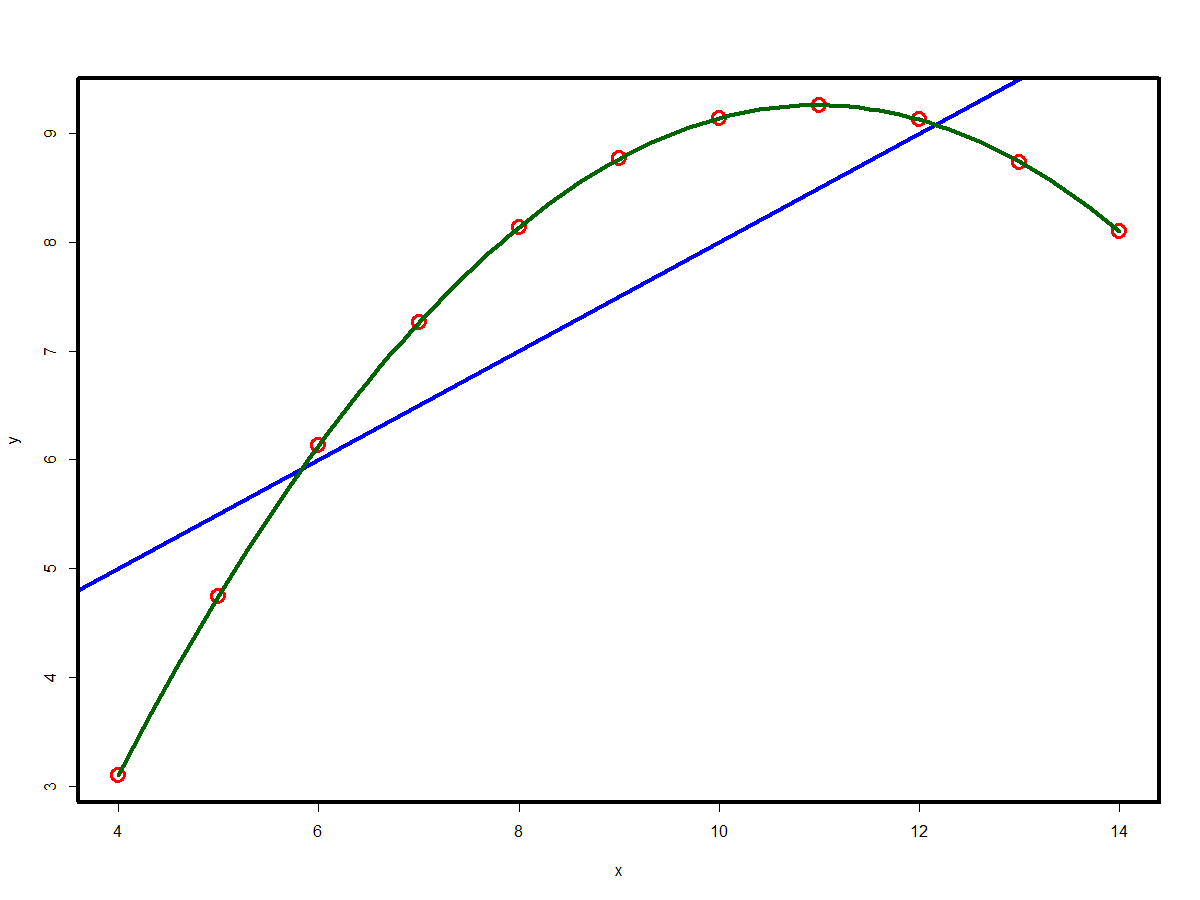
\includegraphics[width=8cm]{../fig/Tut10-09.png}
\begin{knitrout}
\definecolor{shadecolor}{rgb}{0.969, 0.969, 0.969}\color{fgcolor}
\includegraphics[width=\maxwidth]{figure/unnamed-chunk-65-1} 

\end{knitrout}
\end{center}
\caption{Ejemplo de regresión polinómica con R.}
\label{tut10:fig:RegresionPolinomica}
\end{figure}

Terminamos este apartado proponiendo al lector un ejercicio:
\begin{ejercicio}
\label{tut10:ejercicio10}
Vamos a buscar una parábola para los datos del Ejemplo \ref{curso-cap10:ejem:RectaMalaAproximacion01} (pág \pageref{curso-cap10:ejem:RectaMalaAproximacion01}) del libro. Los datos están en el fichero:
\begin{center}
{\tt Cap10-EjemploRectaMalaAproximacion01.csv}
\end{center}
que puedes encontrar en el ejercicio 2(b) de la pág. \pageref{tut10:ejercicio03} de este tutorial. Los valores de ese ejemplo se han generado en R con el código:
\begin{knitrout}
\definecolor{shadecolor}{rgb}{0.969, 0.969, 0.969}\color{fgcolor}\begin{kframe}
\begin{alltt}
\hlkwd{set.seed}\hlstd{(}\hlnum{2013}\hlstd{)}
\hlstd{(x} \hlkwb{=} \hlkwd{signif}\hlstd{(}\hlkwd{runif}\hlstd{(}\hlkwc{n}\hlstd{=}\hlnum{30}\hlstd{,} \hlkwc{min}\hlstd{=}\hlnum{0}\hlstd{,} \hlkwc{max}\hlstd{=}\hlnum{1} \hlstd{),} \hlkwc{digits}\hlstd{=}\hlnum{3}\hlstd{) )}
\hlstd{(y} \hlkwb{=} \hlkwd{signif}\hlstd{(x}\hlopt{-}\hlstd{x}\hlopt{^}\hlnum{2}\hlopt{+}\hlkwd{rnorm}\hlstd{(}\hlnum{30}\hlstd{,}\hlkwc{sd}\hlstd{=}\hlnum{0.001}\hlstd{),}\hlkwc{digits}\hlstd{=}\hlnum{2} \hlstd{) )}
\end{alltt}
\end{kframe}
\end{knitrout}
Eso significa que se basan en un modelo teórico como este:
\[y=\beta_0+\beta_1\cdot x+\beta_2\cdot x^2+\epsilon=x-x^2+\epsilon\]
En el que hemos tomado
\[\beta_0=0, \beta_0=1, \beta_2=-1,\]
y en el que el término de error cumple
\[\epsilon\sim N(30,0.001).\]
Naturalmente, cuando obtengas $b_0$, $b_1$ y $b_2$, sus valores no coincidirán exactamente con los de $\beta_0=0$, $\beta_0=1$ y $\beta_2=-1$, pero deberían ser {\em bastante parecidos}. Para comprobar gráficamente el resultado, dibuja la parábola que obtienes sobre el diagrama de dispersión de los puntos $(x,y)$.
\qed
\end{ejercicio}




%La que he obtenido yo se muestra en la Figura \ref{tut10:fig:RegresionPolinomica}.
%\begin{figure}[h!]
%\begin{center}
%    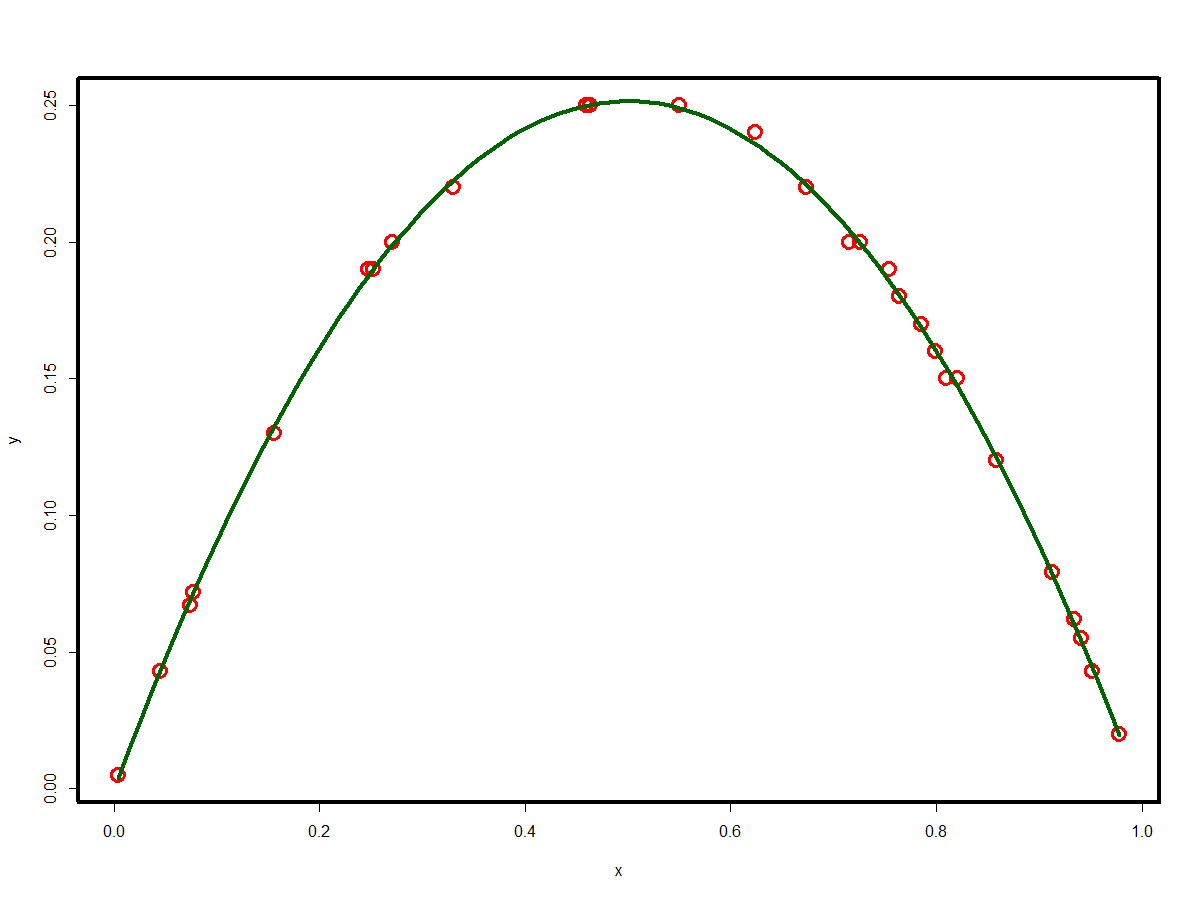
\includegraphics[width=6.5cm]{../fig/Tut10-10.png}
%\end{center}
%\caption{Parábola para los datos del Ejemplo \ref{curso-cap10:ejem:RectaMalaAproximacion01} del libro.}
%\label{tut10:fig:RegresionPolinomica}
%\end{figure}
\qed


\section{Ejercicios adicionales y soluciones.}
\label{tut10:sec:EjerciciosAdicionalesYSoluciones}

\subsection*{Ejercicios adicionales.}
\label{tut10:subsec:EjerciciosAdicionales}

\begin{ejercicio}
\label{tut10:ejercicio11}
El Ejemplo \ref{curso-cap10:ejem:AnalisisGraficoResiduos02} del libro (pág. \pageref{curso-cap10:ejem:AnalisisGraficoResiduos02}) incluye una muestra de puntos para l que la condición de homogeneidad de la varianza claramente no se cumple. Esa muestra de puntos se ha fabricado en R con este código:
\begin{knitrout}
\definecolor{shadecolor}{rgb}{0.969, 0.969, 0.969}\color{fgcolor}\begin{kframe}
\begin{alltt}
\hlkwd{set.seed}\hlstd{(}\hlnum{2013}\hlstd{)}
\hlstd{n}\hlkwb{=}\hlnum{100}
\hlstd{(x} \hlkwb{=} \hlkwd{sort}\hlstd{(}\hlkwd{signif}\hlstd{(}\hlkwd{runif}\hlstd{(n,} \hlkwc{min}\hlstd{=}\hlnum{0}\hlstd{,} \hlkwc{max}\hlstd{=}\hlnum{1} \hlstd{),} \hlkwc{digits}\hlstd{=}\hlnum{2}\hlstd{) )  )}
\hlstd{(y} \hlkwb{=} \hlnum{1} \hlopt{-} \hlstd{(x}\hlopt{/}\hlnum{2}\hlstd{)} \hlopt{+} \hlkwd{rnorm}\hlstd{(n,}\hlkwc{sd}\hlstd{=}\hlnum{0.01}\hlopt{*}\hlstd{(}\hlnum{1}\hlopt{+}\hlnum{50}\hlopt{*}\hlstd{x)))}
\end{alltt}
\end{kframe}
\end{knitrout}

\begin{enumerate}
  \item Dibuja el diagrama de dispersión de esa muestra de puntos.
%  <<fig.width=5, fig.height=5>>=
%  plot(x, y)
%  @
  \item Dibuja también el gráfico de los residuos estudentizados frente a los valores predichos que aparece en la parte (b) de la Figura \ref{curso-cap10:fig:AnalisisMedianteResiduosHomogeneidadVarianza} del libro (pág. \pageref{curso-cap10:fig:AnalisisMedianteResiduosHomogeneidadVarianza}). Para facilitarte el trabajo, los residuos estudentizados se pueden obtener con la función {\tt studres} de la librería {\tt MASS}, aplicada al modelo lineal que se obtiene con \verb#lm(y ~ x)#. Y recuerda que los valores predichos son la componente {\tt fitted.values} de la salida de la función {\tt lm}.

  \item Aplica la función {\tt gvlma} (de la librería homónima) al modelo lineal para ver los diagnósticos que proporciona.

  \item Por último, ¿por qué sucede esto? Busca una explicación en la forma en la que se han construido los valores $y$ a partir de los valores $x$.
\end{enumerate}
\qed
\end{ejercicio}

\begin{ejercicio}
\label{tut10:ejercicio12}
Comprueba los resultados del Ejemplo \ref{curso-cap10:ejem:RegresionPolinomica} del libro (pág. \pageref{curso-cap10:ejem:RegresionPolinomica}).
\qed
\end{ejercicio}



%%##########################################
%##########################################

\subsection*{Soluciones de algunos ejercicios.}
\label{tut10:subsec:SolucionesAlgunosEjercicios}


\paragraph{\bf $\bullet$ Ejercicio \ref{tut10:ejercicio01}, pág. \pageref{tut10:ejercicio01}}
\label{tut10:ejercicio01:sol}\quad\\


\begin{enumerate}
  \item
  Este es el caso más simple:
  {\small
\begin{knitrout}
\definecolor{shadecolor}{rgb}{0.969, 0.969, 0.969}\color{fgcolor}\begin{kframe}
\begin{alltt}
\hlstd{(datos} \hlkwb{=} \hlkwd{read.table}\hlstd{(}\hlstr{"../datos/tut10-ejercicio01-1.csv"}\hlstd{,} \hlkwc{sep}\hlstd{=}\hlstr{","}\hlstd{,} \hlkwc{header}\hlstd{=}\hlnum{TRUE}\hlstd{))}
\end{alltt}
\begin{verbatim}
##     x     y
## 1 0.9  0.63
## 2 1.4  4.38
## 3 1.8  5.86
## 4 1.9  6.43
## 5 2.3  7.81
## 6 2.5 10.05
## 7 2.6  9.02
## 8 2.9 11.23
\end{verbatim}
\end{kframe}
\end{knitrout}
  }
  \item Basta con modificar la opción {\tt sep}:
  {\small
\begin{knitrout}
\definecolor{shadecolor}{rgb}{0.969, 0.969, 0.969}\color{fgcolor}\begin{kframe}
\begin{alltt}
\hlstd{(datos} \hlkwb{=} \hlkwd{read.table}\hlstd{(}\hlstr{"../datos/tut10-ejercicio01-2.csv"}\hlstd{,} \hlkwc{sep}\hlstd{=}\hlstr{"\textbackslash{}t"}\hlstd{,} \hlkwc{dec}\hlstd{=}\hlstr{","}\hlstd{,} \hlkwc{header}\hlstd{=}\hlnum{TRUE}\hlstd{))}
\end{alltt}
\begin{verbatim}
##     x     y
## 1 0.9  0.63
## 2 1.4  4.38
## 3 1.8  5.86
## 4 1.9  6.43
## 5 2.3  7.81
## 6 2.5 10.05
## 7 2.6  9.02
## 8 2.9 11.23
\end{verbatim}
\end{kframe}
\end{knitrout}
  }
  \item En este caso el fichero de datos está organizado de una manera especialmente molesta, con los datos dispuestos en filas en lugar de columnas, separados por punto y coma, y usando comas para los decimales. Pero con R podemos salir del paso sin demasiadas complicaciones. Los siguientes comandos te permitirán leer los datos y guardarlos en un {\tt data.frame} idéntico al de los apartados anteriores:
      {\small
\begin{knitrout}
\definecolor{shadecolor}{rgb}{0.969, 0.969, 0.969}\color{fgcolor}\begin{kframe}
\begin{alltt}
\hlstd{datos} \hlkwb{=} \hlkwd{read.table}\hlstd{(}\hlstr{"../datos/tut10-ejercicio01-3.csv"}\hlstd{,} \hlkwc{sep}\hlstd{=}\hlstr{";"}\hlstd{,} \hlkwc{dec}\hlstd{=}\hlstr{","}\hlstd{)}
\hlstd{datos} \hlkwb{=} \hlkwd{t}\hlstd{(}\hlkwd{as.matrix}\hlstd{(datos[ ,} \hlopt{-}\hlnum{1}\hlstd{]))}
\hlstd{datos} \hlkwb{=} \hlkwd{data.frame}\hlstd{(datos,} \hlkwc{row.names} \hlstd{=} \hlkwa{NULL}\hlstd{)}
\hlkwd{colnames}\hlstd{(datos)} \hlkwb{=} \hlkwd{c}\hlstd{(}\hlstr{"x"}\hlstd{,} \hlstr{"y"}\hlstd{)}
\hlstd{datos}
\end{alltt}
\begin{verbatim}
##     x     y
## 1 0.9  0.63
## 2 1.4  4.38
## 3 1.8  5.86
## 4 1.9  6.43
## 5 2.3  7.81
## 6 2.5 10.05
## 7 2.6  9.02
## 8 2.9 11.23
\end{verbatim}
\end{kframe}
\end{knitrout}
    }
    El paso clave es el segundo, en el que leemos la parte numérica de los datos como una matriz usamos {\tt datos[ , -1]} para {\em excluir} la primera columna), y la trasponemos con la función {\tt t}.
\end{enumerate}


\paragraph{\bf $\bullet$ Ejercicio \ref{tut10:ejercicio02}, pág. \pageref{tut10:ejercicio02}}
\label{tut10:ejercicio02:sol}\quad\\


\begin{enumerate}
  \item La fórmula de la Ecuación \ref{curso-cap10:ecu:CoeficienteRegresionPearson}  del libro se obtiene con:
\begin{knitrout}
\definecolor{shadecolor}{rgb}{0.969, 0.969, 0.969}\color{fgcolor}\begin{kframe}
\begin{alltt}
\hlkwd{with}\hlstd{(datosPisa, \{}
  \hlkwd{cov}\hlstd{(rpc, pisa)}\hlopt{/}\hlstd{(}\hlkwd{sd}\hlstd{(rpc)} \hlopt{*} \hlkwd{sd}\hlstd{(pisa))}
  \hlstd{\})}
\end{alltt}
\end{kframe}
\end{knitrout}
  \item Ejecutando
  \begin{verbatim}
    CoeficienteCorrelación[datosPisa]
  \end{verbatim}
  obtenemos $0.75277$, de acuerdo con lo que se obtiene en R.
\end{enumerate}


%#########################################################################################
%#########################################################################################
\vspace{2cm} \hrule
\quad\\
Fin del Tutorial10. ¡Gracias por la atención!

%\newpage
%\addcontentsline{toc}{section}{Guía de trabajo.}
%\includepdf[pages={1-},scale=0.90]{10-GuiaDeTrabajo.pdf}






\end{document}



